%%%%%%%%%%%%%%%%%%%%%%%%%%%%%%%%%%%%%%%%%%%%%%%%%%%%%%%%%%%%%%%%%%%%%%%%%%%%%%%%%%%%%%%%%%%%%%%%%%%%%%
%
%   Filename    : chapter_7.tex 
%
%   Description : This file will contain details of the chatp7.1cussion of the study.
%                 
%%%%%%%%%%%%%%%%%%%%%%%%%%%%%%%%%%%%%%%%%%%%%%%%%%%%%%%%%%%%%%%%%%%%%%%%%%%%%%%%%%%%%%%%%%%%%%%%%%%%%%

\chapter{Results and Discussion}

This section explores and presents the evaluation results and improvements made to the fine-tuned YOLOv11-Large Instance Segmentation Model, the Mobile Application designed and developed to collect user experiences and cycling trips, as well as the implementation of the WeCyclePH crowdsourcing system for data collection. First, the YOLOv11 model was fine-tuned from a dataset of annotated YouTube videos, enhancing its capabilities to efficiently detect and segment particularly non-vehicular objects, such as potholes, barriers, debris, and the like. Second, the design and development of the mobile application had undergone a series of user testing, such as guerrilla testing (i.e., to assess initial usability and intuitiveness), closed beta testing (i.e., to evaluate performance and usability), and user acceptance testing (i.e., to evaluate whether the app meets the users' needs), in which multiple iterations of app rework have been performed in between based on the significant findings identified from each testing phase. Finally, the implementation of the WeCyclePH system performed real-world data collection, combining data obtained from users' cycling trips along with their crowdsourced annotations, including video-based road analysis from the trained deep learning segmentation model.

\section{Instance Segmentation Model}
\subsection{Model Evaluation}
The instance segmentation model was evaluated on a test set consisting of 370 images containing 1,763 annotated instances across 10 object classes. The overall performance metrics indicate moderate success in object detection and segmentation, with a box-level mean Average Precision at 50\% IoU threshold (\textbf{mAP@50}) of \textbf{0.398} and a stricter averaged score across multiple IoU thresholds from 50\% to 95\% (\textbf{mAP@50–95}) of \textbf{0.298}. Mask-level performance was slightly lower, with \textbf{mAP@50} at \textbf{0.387} and \textbf{mAP@50–95} at \textbf{0.264}, suggesting the model was generally better at object detection than pixel-level segmentation, though both performances are relatively aligned.

Among individual classes, \texttt{jeepney} and \texttt{tricycle} demonstrated the highest segmentation performance, with \texttt{jeepney} achieving a mask mAP@50 of \textbf{0.687} and mAP@50–95 of \textbf{0.486}, and \texttt{tricycle} reaching \textbf{0.618} and \textbf{0.402}, respectively. These results suggest the model is highly capable of distinguishing these uniquely shaped and culturally specific vehicle types in the Philippine urban context, likely due to the distinct visual features and relatively consistent annotation quality for these classes.

Conversely, the model underperformed on more challenging or underrepresented classes such as \texttt{bicycle}, which recorded the lowest mAP scores—mask mAP@50 of \textbf{0.21} and mAP@50–95 of only \textbf{0.0804}. This reflects difficulty in detecting and segmenting cyclists, possibly due to limited training samples, class ambiguity (e.g., overlap with motorcycles), and high intra-class variation (e.g., riding positions, occlusions). Similarly, \texttt{person} detection showed poor recall (0.039 for box and 0.0355 for mask) despite a relatively high precision, indicating the model often failed to detect individuals when present—an issue that limits its utility in analyzing pedestrian-cyclist interactions or shared space safety.

The \texttt{bike\_lane} class, a critical feature for this study, performed moderately well with a mask mAP@50 of \textbf{0.501} and mAP@50–95 of \textbf{0.44}, which indicates the model can detect and segment bike lane markings with reasonable accuracy. However, the low recall values suggest that while the model is precise when it predicts a bike lane, it frequently misses them—highlighting the need for further improvement through additional training data or augmentation specific to lane features.

Overall, while certain classes like \texttt{jeepney}, \texttt{tricycle}, and \texttt{bike\_lane} show promising detection and segmentation results, the model's performance across several other critical classes, such as \texttt{bicycle}, \texttt{person}, and \texttt{barrier}, remains limited. The moderate overall mAP values indicate the model is suitable for exploratory analysis but requires refinement for deployment in decision-making or real-time urban monitoring systems.

\begin{table}[h!]
\centering
\resizebox{\textwidth}{!}{%
\begin{tabular}{lrrrrrrrrrr}
\hline
\textbf{Class} & \textbf{Images} & \textbf{Instances} & \textbf{Box P} & \textbf{Box R} & \textbf{Box mAP50} & \textbf{Box mAP50-95} & \textbf{Mask P} & \textbf{Mask R} & \textbf{Mask mAP50} & \textbf{Mask mAP50-95} \\
\hline
\textbf{all}        & 370 & 1763 & 0.579 & 0.274 & 0.398 & 0.298 & 0.568 & 0.271 & 0.387 & 0.264 \\
car                 & 222 & 644  & 0.657 & 0.149 & 0.402 & 0.349 & 0.657 & 0.149 & 0.399 & 0.310 \\
tricycle            & 28  & 34   & 0.509 & 0.618 & 0.644 & 0.527 & 0.509 & 0.618 & 0.618 & 0.402 \\
truck               & 67  & 83   & 0.497 & 0.217 & 0.271 & 0.192 & 0.497 & 0.217 & 0.280 & 0.173 \\
bicycle             & 66  & 76   & 0.276 & 0.145 & 0.171 & 0.0877 & 0.326 & 0.171 & 0.210 & 0.0804 \\
motorcycle          & 145 & 245  & 0.598 & 0.291 & 0.405 & 0.196 & 0.556 & 0.271 & 0.346 & 0.151 \\
bike\_lane          & 172 & 173  & 0.844 & 0.282 & 0.512 & 0.424 & 0.827 & 0.277 & 0.501 & 0.440 \\
barrier             & 55  & 74   & 0.328 & 0.230 & 0.249 & 0.129 & 0.289 & 0.203 & 0.224 & 0.120 \\
bus                 & 41  & 51   & 0.453 & 0.275 & 0.356 & 0.308 & 0.453 & 0.275 & 0.356 & 0.298 \\
person              & 130 & 282  & 0.723 & 0.039 & 0.273 & 0.193 & 0.657 & 0.0355 & 0.253 & 0.177 \\
jeepney             & 67  & 101  & 0.908 & 0.491 & 0.696 & 0.570 & 0.908 & 0.491 & 0.687 & 0.486 \\
\hline
\end{tabular}
}
\caption{YOLOv11 evaluation results: Precision (P), Recall (R), mAP@0.5, and mAP@0.5:0.95 for Bounding Box and Segmentation Mask across classes.}
\label{tab:yolov11_results}
\end{table}

\subsection{Losses}

\subsubsection{Box Loss}
The box loss curve shows a clear case of overfitting. The training box loss (dark blue) steadily and smoothly decreases over epochs, indicating that the model is learning to better localize object bounding boxes on the training set. However, the validation box loss (orange) starts high, fluctuates early on, and then plateaus around 1.1–1.2, with no significant downward trend. This gap between training and validation loss—especially as the training loss approaches 0.2—suggests that while the model fits the training data well, it fails to generalize to unseen validation samples. This mismatch could be due to overfitting, limited diversity or quantity in the validation set, or poorly represented box annotations in the data.

\begin{figure}[H]
    \centering
    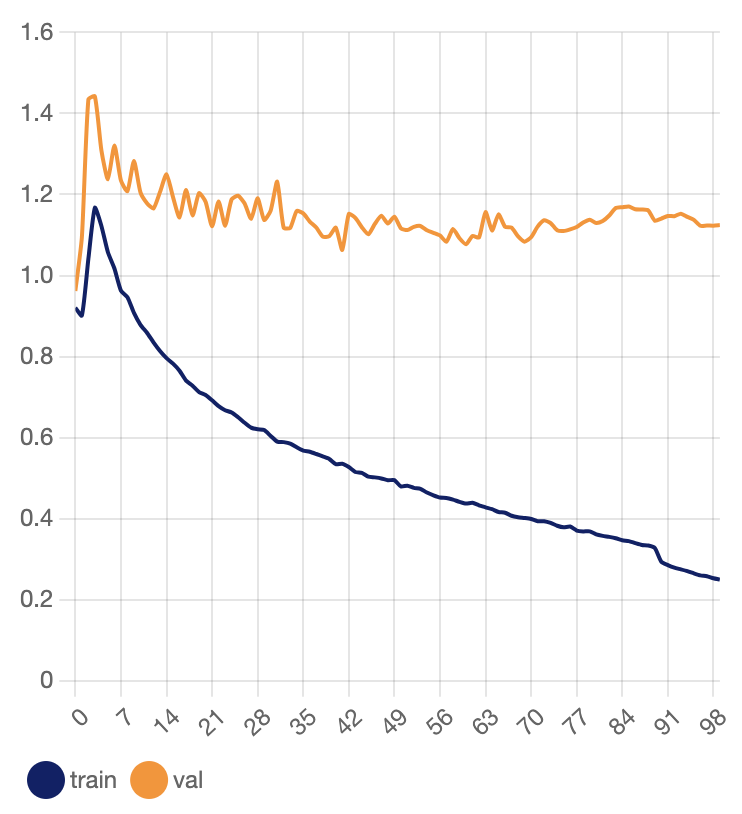
\includegraphics[width=0.5\linewidth]{figures/chapt7/section7.1/box_loss.png}
    \caption{Box loss after fine-tuning the YOLOv11l instance segmentation model}
    \label{fig:box_loss}
\end{figure}

\subsubsection{Class Loss}
The class loss curve also indicates severe overfitting. While the training class loss steadily decreases and approaches near-zero, the validation class loss increases consistently, peaking around 4.0. This suggests the model has learned to classify training data well but fails to generalize to unseen data. The divergence may be caused by class imbalance, label noise, insufficient validation samples, or lack of regularization.

\begin{figure}[H]
    \centering
    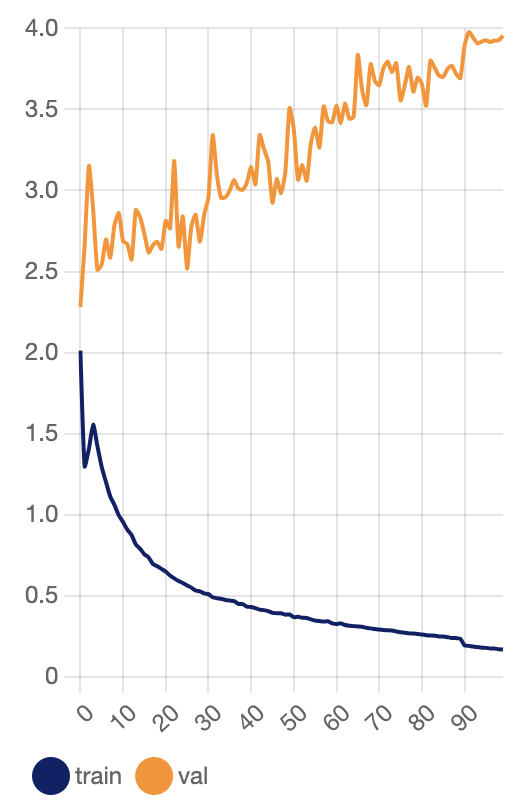
\includegraphics[width=0.5\linewidth]{figures/chapt7/section7.1/class_loss.png}
    \caption{Class loss after fine-tuning the YOLOv11l Instance Segmentation Model}
    \label{fig:class_loss}
\end{figure}

\subsubsection{Object Loss}
The object loss curve reveals the fine-tuned model to be overfitting. The training loss (dark blue) steadily decreases over epochs, indicating that the model is learning to detect objects more accurately on the training set. In contrast, the validation loss (orange) starts high, fluctuates significantly, and remains consistently elevated throughout training without a clear downward trend. This suggests that while the model performs better on training data, it struggles to generalize to unseen validation data—likely due to issues like insufficient data variety, class imbalance, or domain mismatch between training and validation sets.

\begin{figure}[H]
    \centering
    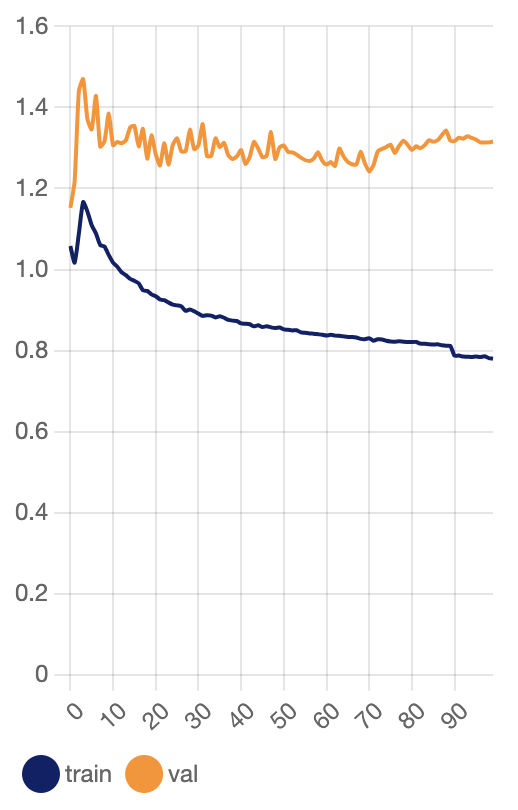
\includegraphics[width=0.5\linewidth]{figures/chapt7/section7.1/object_loss.png}
    \caption{Object loss after fine-tuning the YOLO11l instance segmentation model}
    \label{fig:object_loss}
\end{figure}

\subsection{Confusion Matrix}
The Normalized Confusion Matrix, shown in Figure~\ref{fig:confusion} provides insight into how well the model classifies each object category and how frequently it misclassifies certain objects from the test set.The diagonal values indicate the model's accuracy in predicting each class, with \texttt{tricycle} and \texttt{jeepney} showing the highest correct classification rate of 0.59 and 0.45, respectively. Other classes, such as \texttt{motorcyle} (0.26), \texttt{bike\_lane} (0.24), and \texttt{bus} (0.27) have relatively moderate accuracy, but there are notable misclassifications.

\begin{figure}[H]
    \centering
    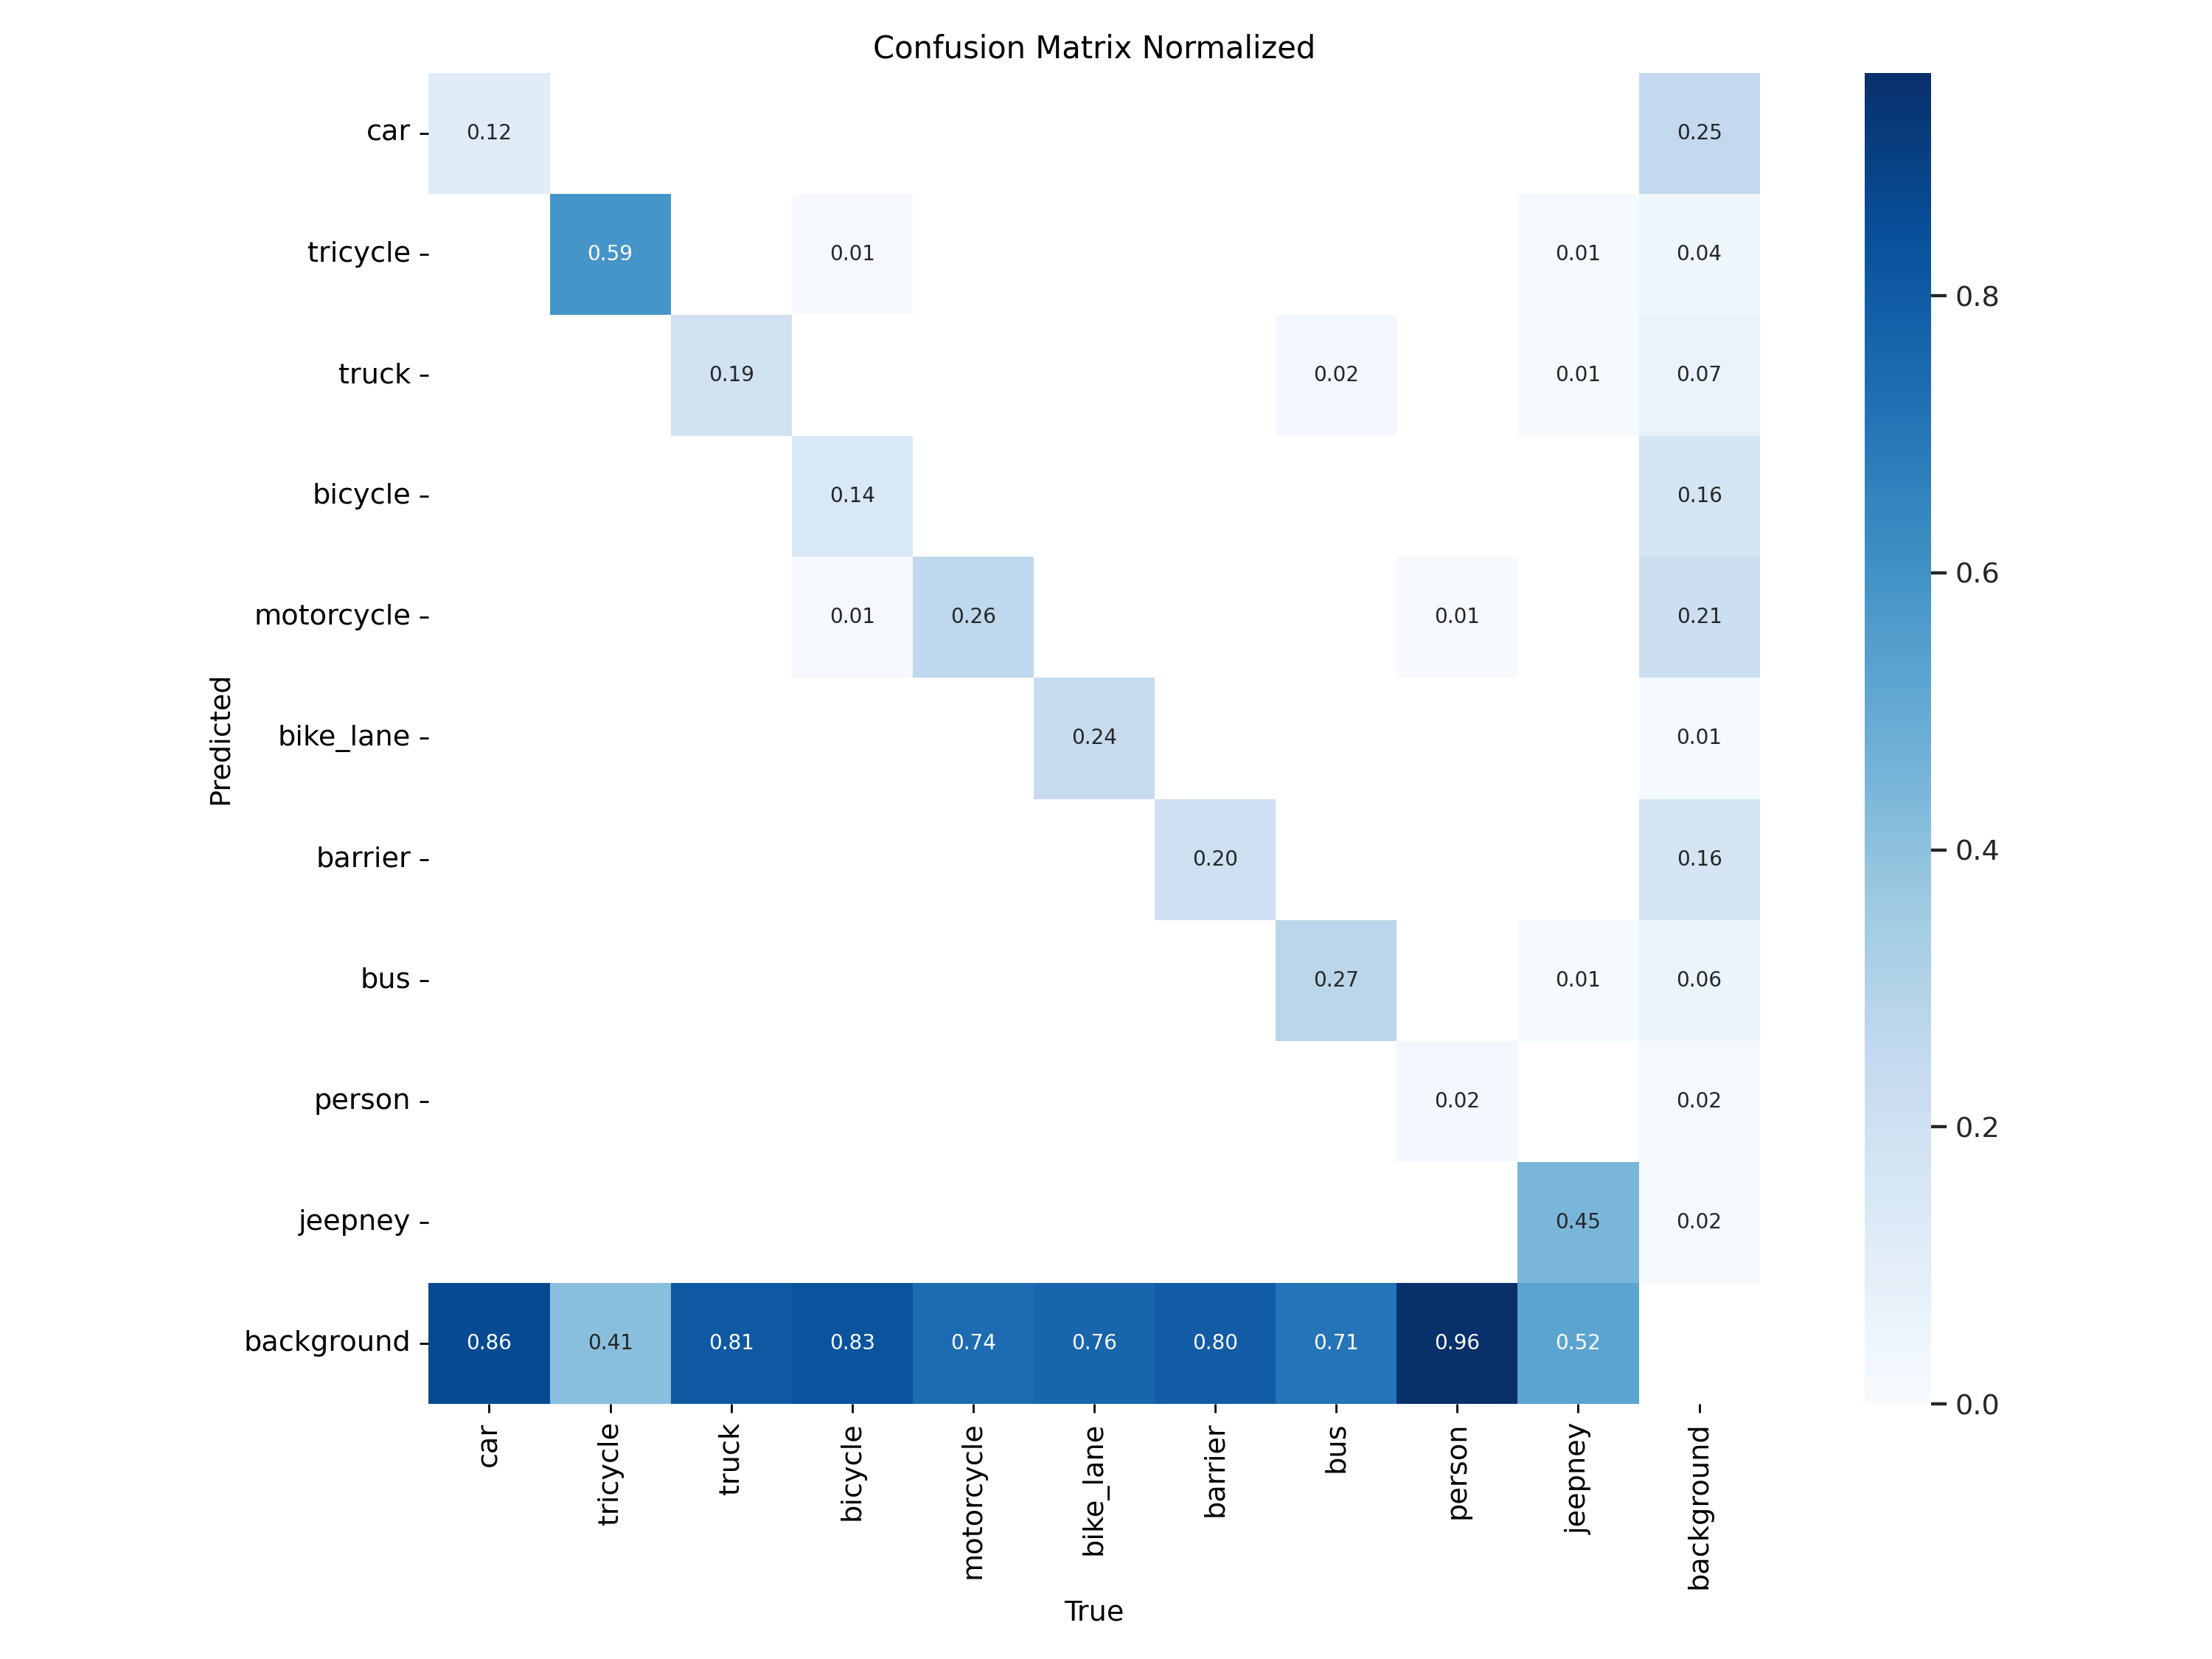
\includegraphics[width=0.75\linewidth]{figures/chapt7/section7.1/confusion_matrix_normalized.png}
    \caption{Normalized confusion matrix of the fine-tuned YOLOv11l model based on the test set}
    \label{fig:confusion}
\end{figure}

For example, \texttt{bus} is confused with jeepney (0.01), while \texttt{motorcycle} is misclassified as \texttt{bicycle} (0.01)—as shown in Figure~\ref{fig:misclassification-confusion}. Other noise in the confusion matrix was towards misclassifying \texttt{bus} as \texttt{truck} (0.02), bicycle as tricycle (0.01), and even jeepney as \texttt{truck} (0.01) or \texttt{tricycle} (0.01).

% Misclassficiation
\begin{figure}[H]
    \centering
    % First image
    \begin{subfigure}[t]{0.48\textwidth}
        \centering
        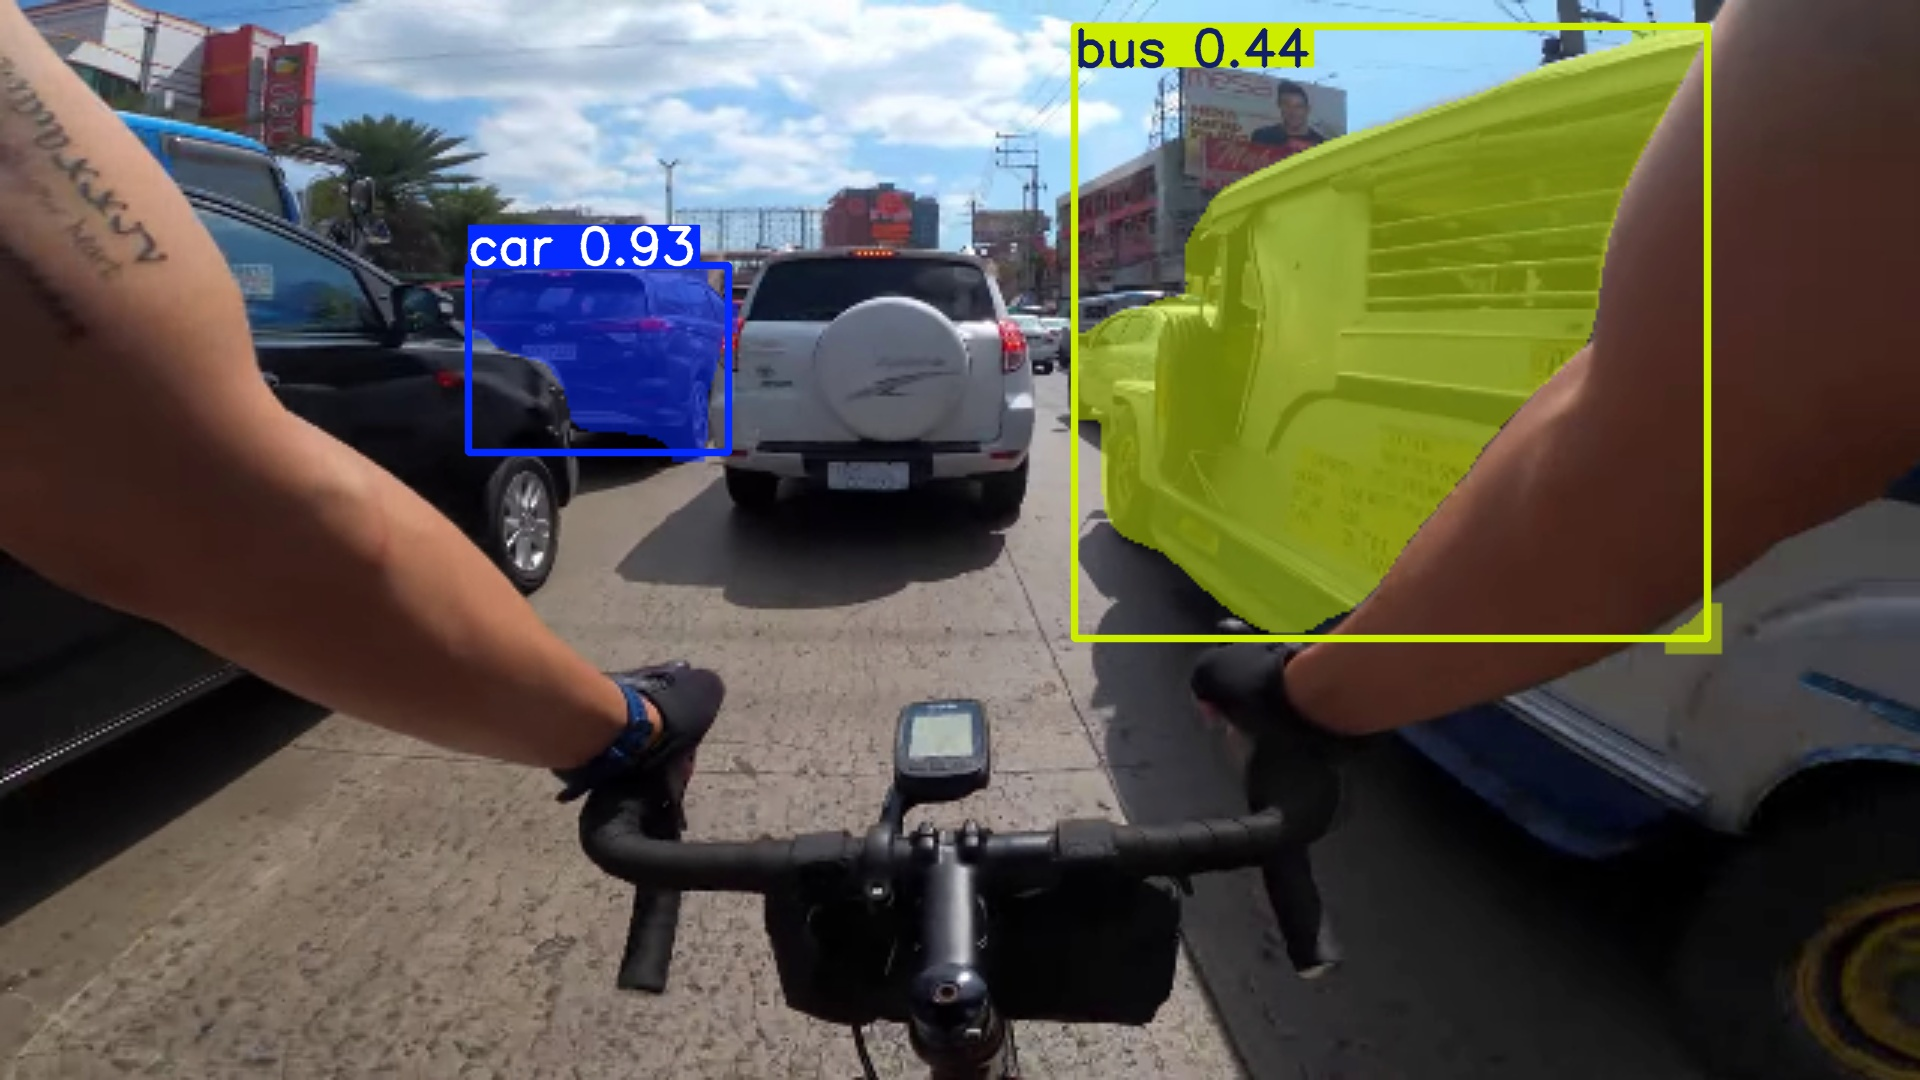
\includegraphics[width=\linewidth]{figures/chapt7/section7.1/inferred_frame_0024.jpg}
        \caption{Misclassification of a \texttt{jeepney} instance to \texttt{bus}}
        \label{fig:first}
    \end{subfigure}
    \hfill
    % Second image
    \begin{subfigure}[t]{0.48\textwidth}
        \centering
        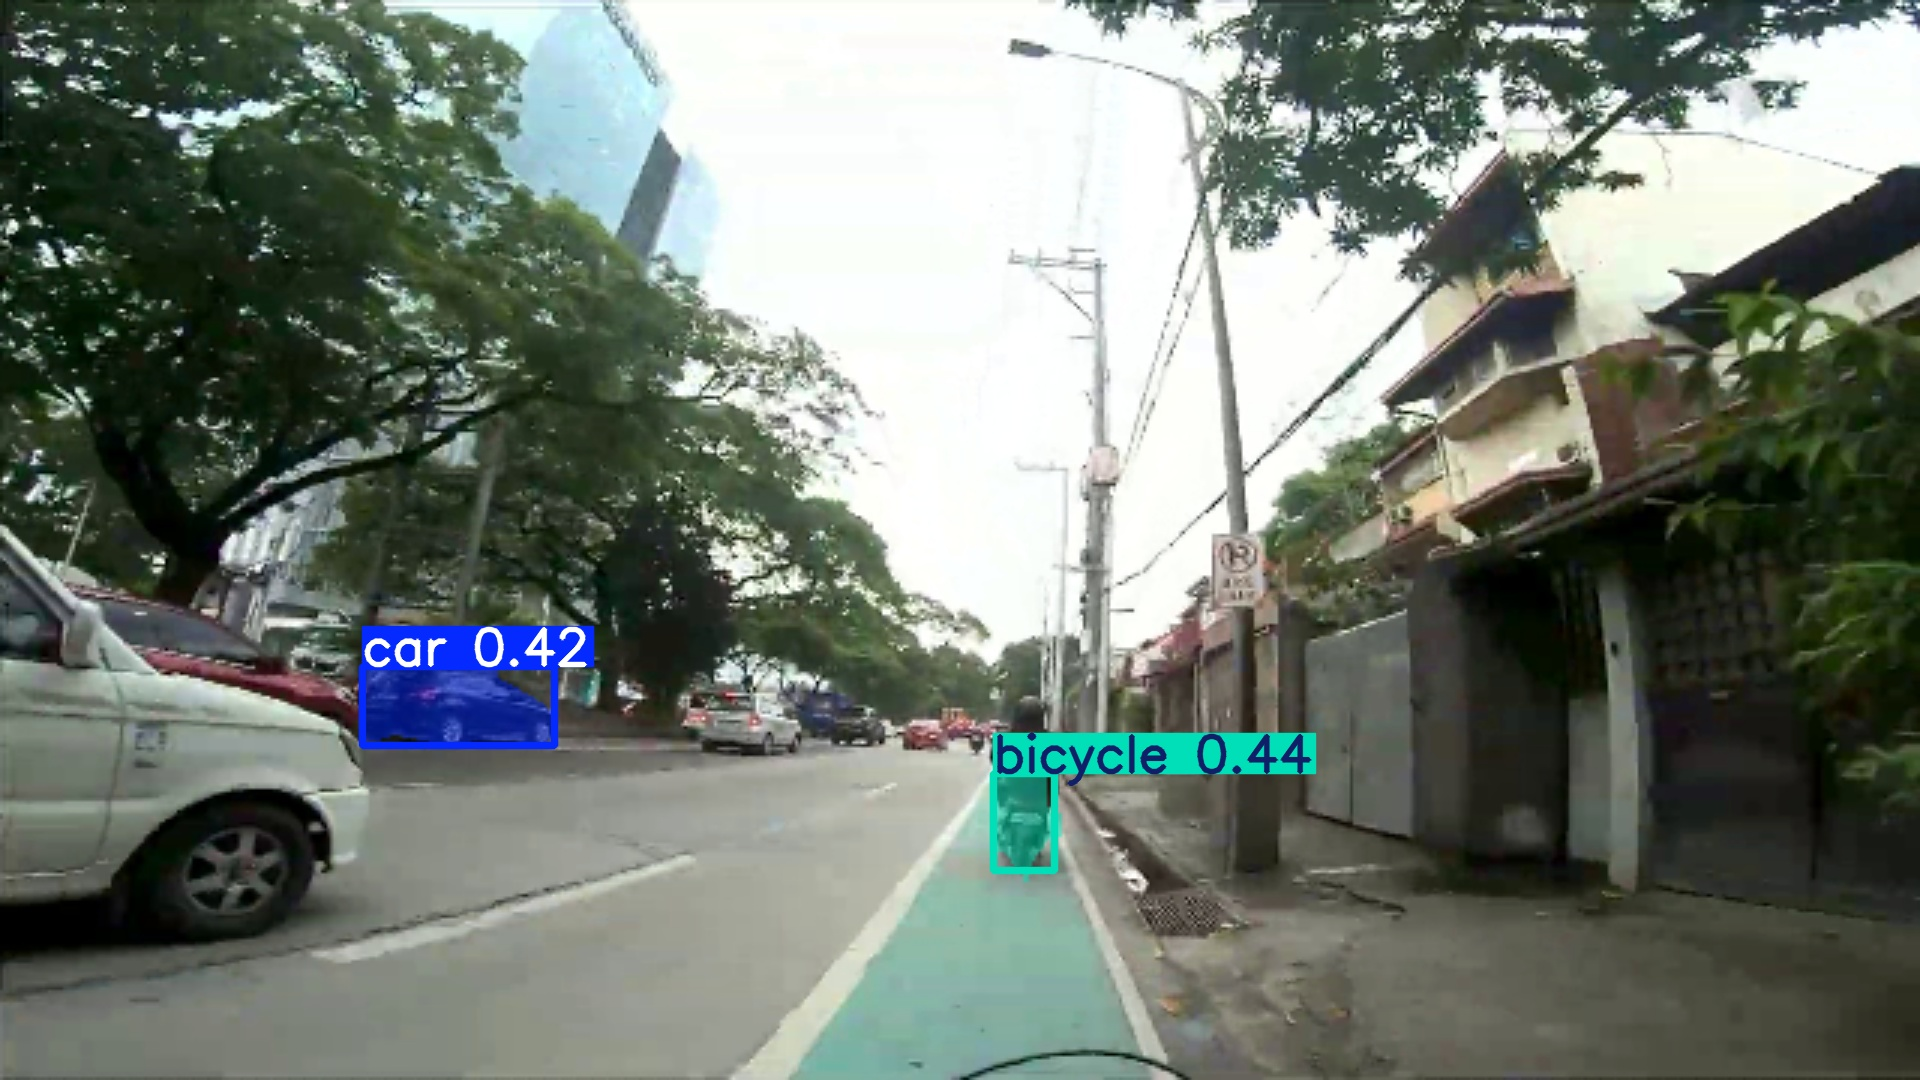
\includegraphics[width=\linewidth]{figures/chapt7/section7.1/inferred_frame_0050.jpg}
        \caption{Misclassification of a  \texttt{motorcycle} instance to \texttt{bicycle}}
        \label{fig:second}
    \end{subfigure}
    \caption{Sample misclassifications identified among classes}
    \label{fig:misclassification-confusion}
\end{figure}

The background class is particularly dominant, with high accuracy rates in distinguishing it from other objects, but it also frequently misclassifies \texttt{car} (0.86), \texttt{truck} (0.81), \texttt{bicycle} (0.83), \texttt{barrier} (0.80), and \texttt{person} (0.96)—as shown in Figure~\ref{fig:background-confusion}.

% Background Classification
\begin{figure}[H]
    \centering
    % First image
    \begin{subfigure}[t]{0.48\textwidth}
        \centering
        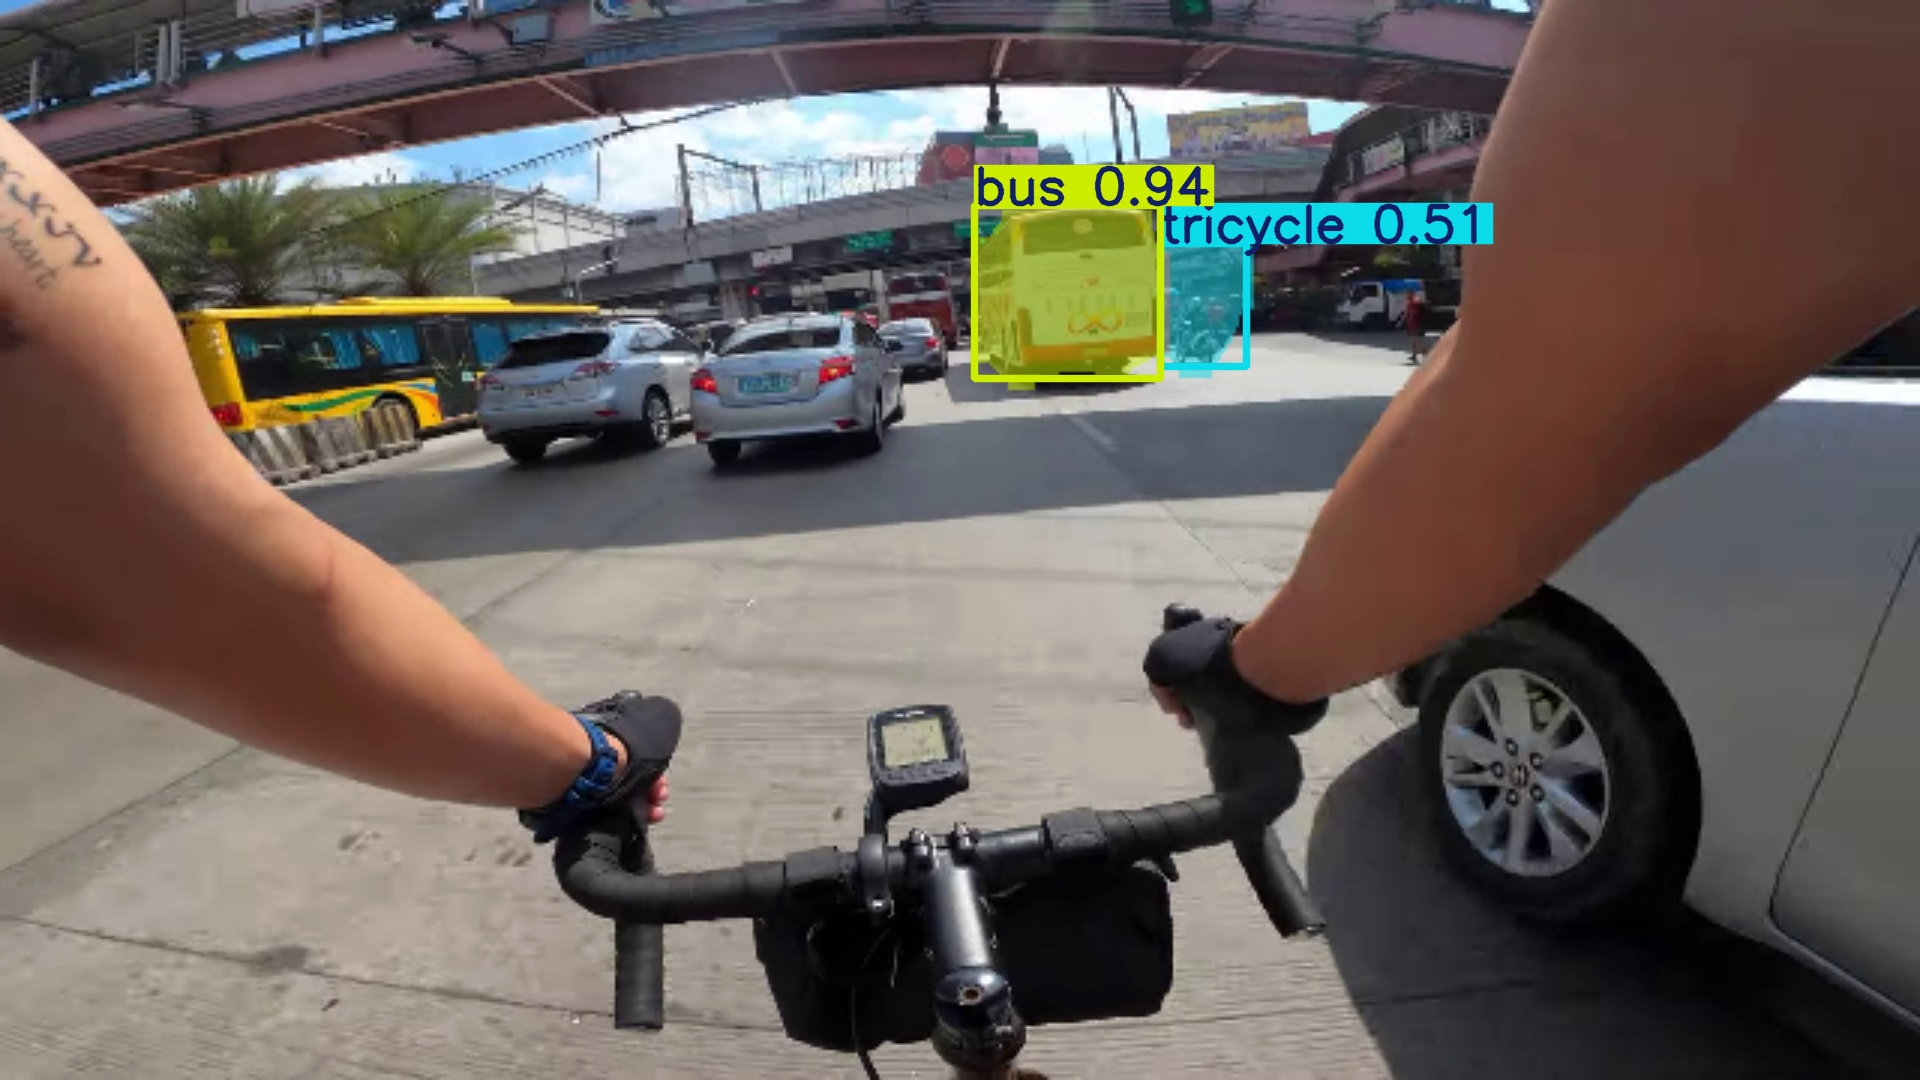
\includegraphics[width=\linewidth]{figures/chapt7/section7.1/inferred_frame_0029.jpg}
        \caption{Misclassification of \texttt{car} instances as background}
        \label{fig:first}
    \end{subfigure}
    \hfill
    % Second image
    \begin{subfigure}[t]{0.48\textwidth}
        \centering
        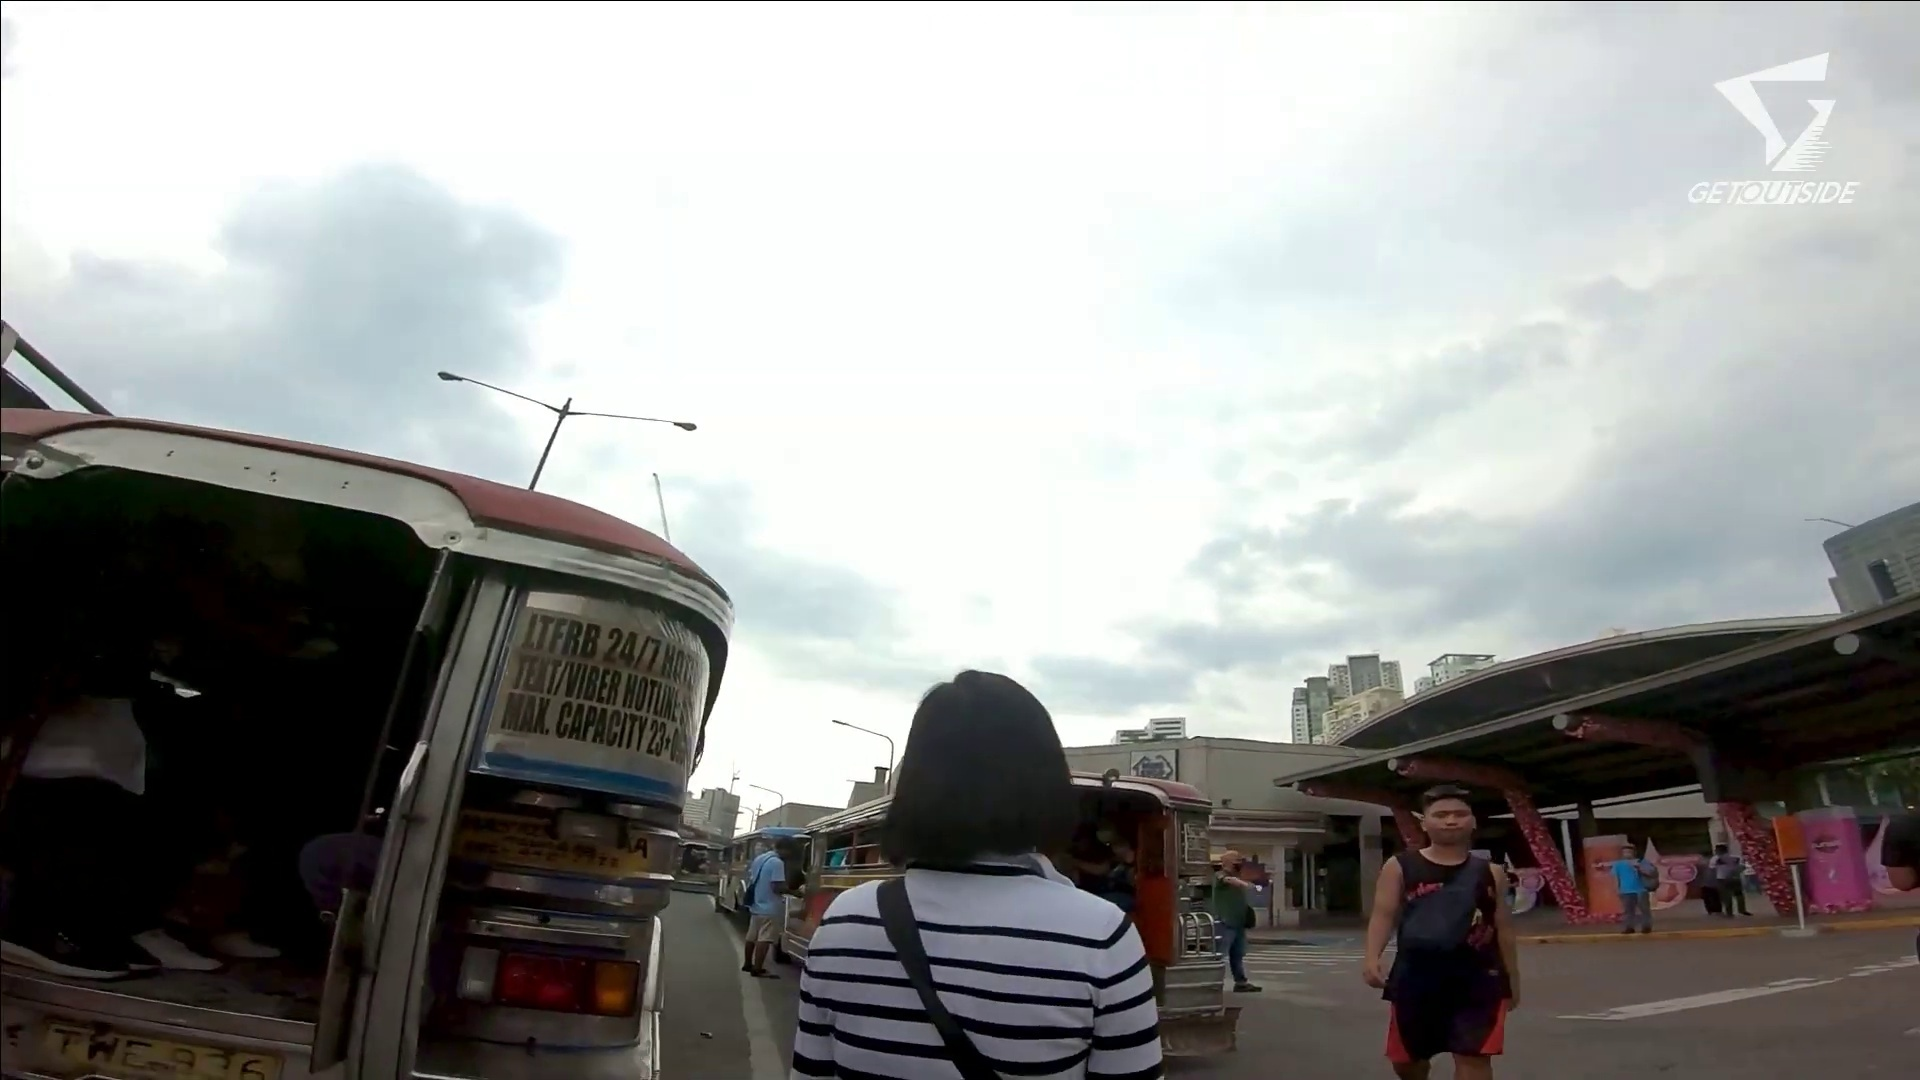
\includegraphics[width=\linewidth]{figures/chapt7/section7.1/inferred_frame_0180.jpg}
        \caption{Misclassification of \texttt{person} instances as background}
        \label{fig:second}
    \end{subfigure}
    \caption{Sample misclassifications of objects as background}
    \label{fig:background-confusion}
\end{figure}

The overall pattern shows that while the model performs well for certain classes like \texttt{jeepney} and \texttt{tricycle} (with examples shown in Figure~\ref{fig:good-confusion}), it struggles with others like \texttt{car}, \texttt{person}, \texttt{bicycle}, and \texttt{truck}, and often misclassifies objects as background.

% Good Classification
\begin{figure}[H]
    \centering
    % First image
    \begin{subfigure}[t]{0.48\textwidth}
        \centering
        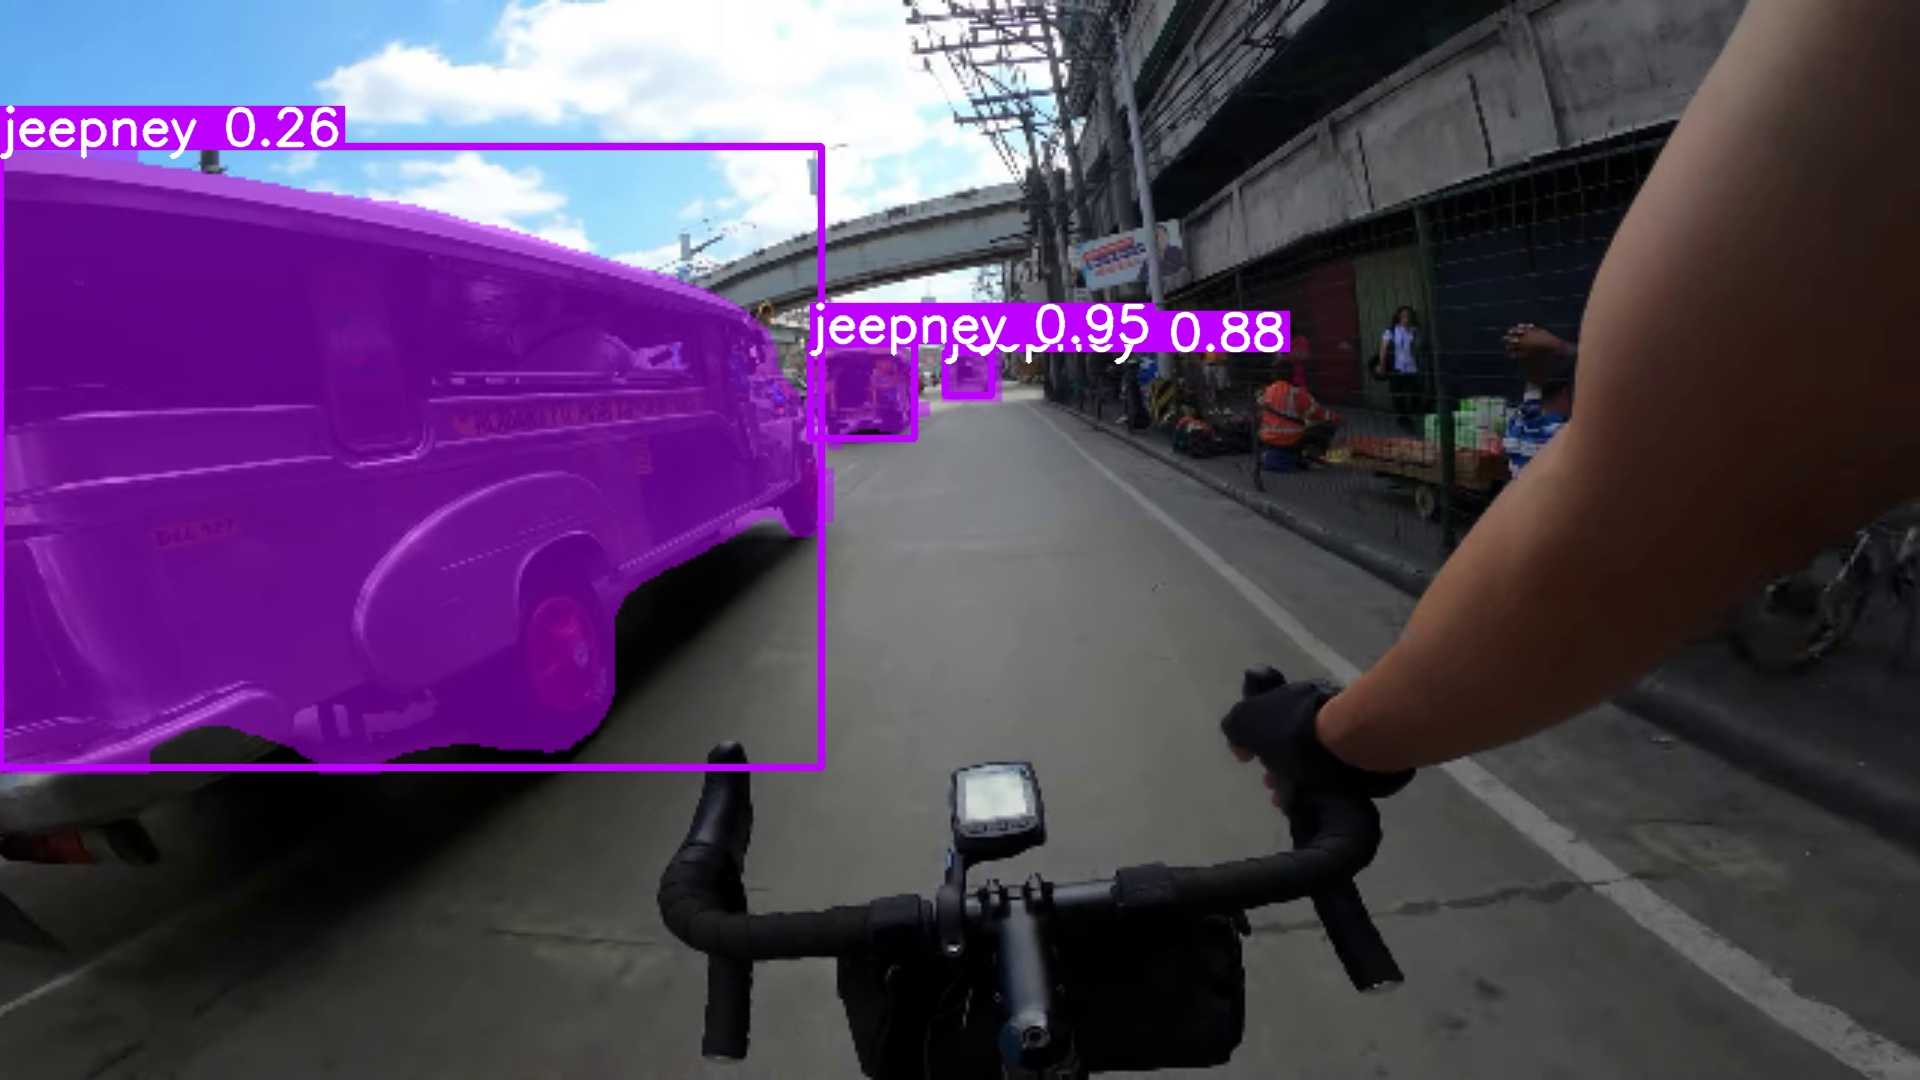
\includegraphics[width=\linewidth]{figures/chapt7/section7.1/inferred_frame_0039.jpg}
        \caption{Good classification on \texttt{jeepney} class}
        \label{fig:first}
    \end{subfigure}
    \hfill
    % Second image
    \begin{subfigure}[t]{0.48\textwidth}
        \centering
        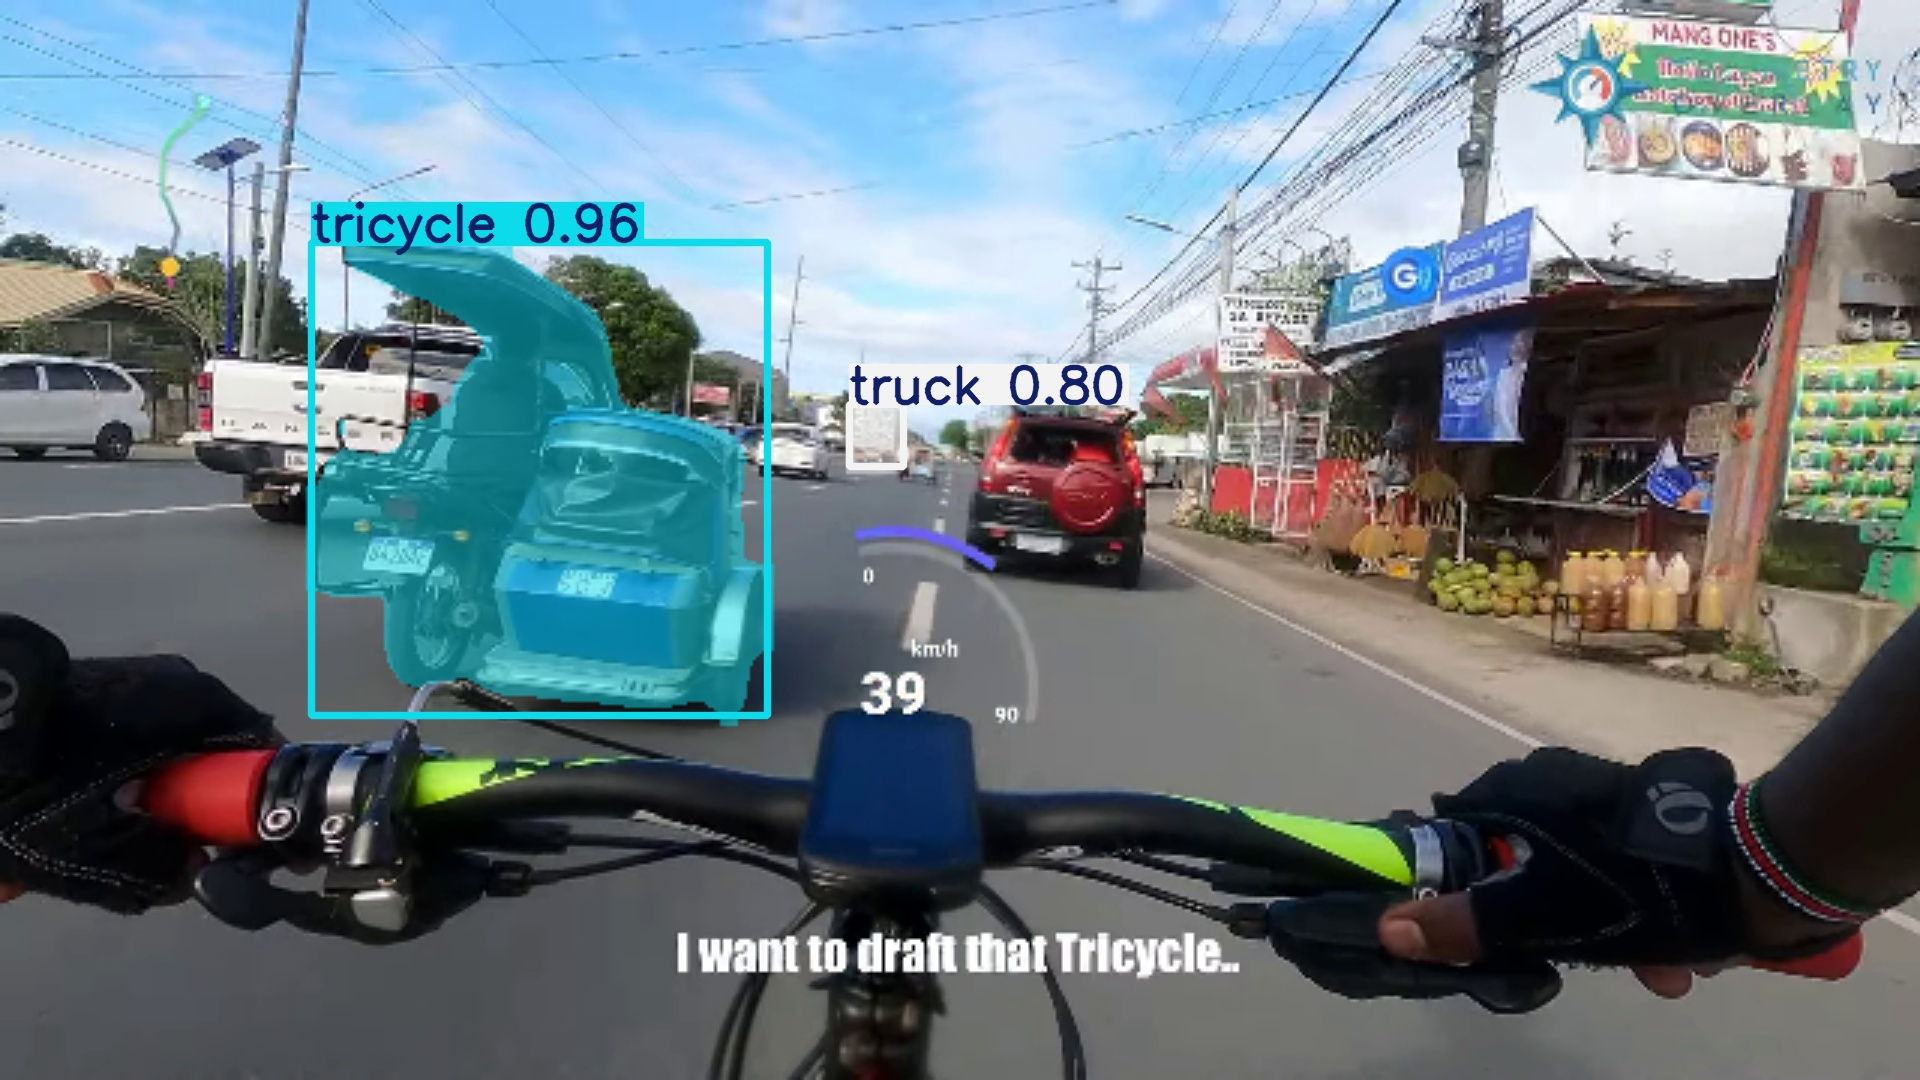
\includegraphics[width=\linewidth]{figures/chapt7/section7.1/inferred_frame_0001.jpg}
        \caption{Good classification on \texttt{tricycle} class}
        \label{fig:second}
    \end{subfigure}
    \caption{Sample misclassifications identified among classes}
    \label{fig:good-confusion}
\end{figure}

These trends suggest that further model refinement is needed to improve the performance across more diverse object categories, particularly for smaller or less distinct classes.

\subsection{Precision}

\subsubsection{Box}
The Precision-Confidence Curve seen in Figure~\ref{fig:precision-curve-box} shows the relationship between the model's confidence in its predictions and the corresponding precision across various object classes.

\begin{figure}[H]
    \centering
    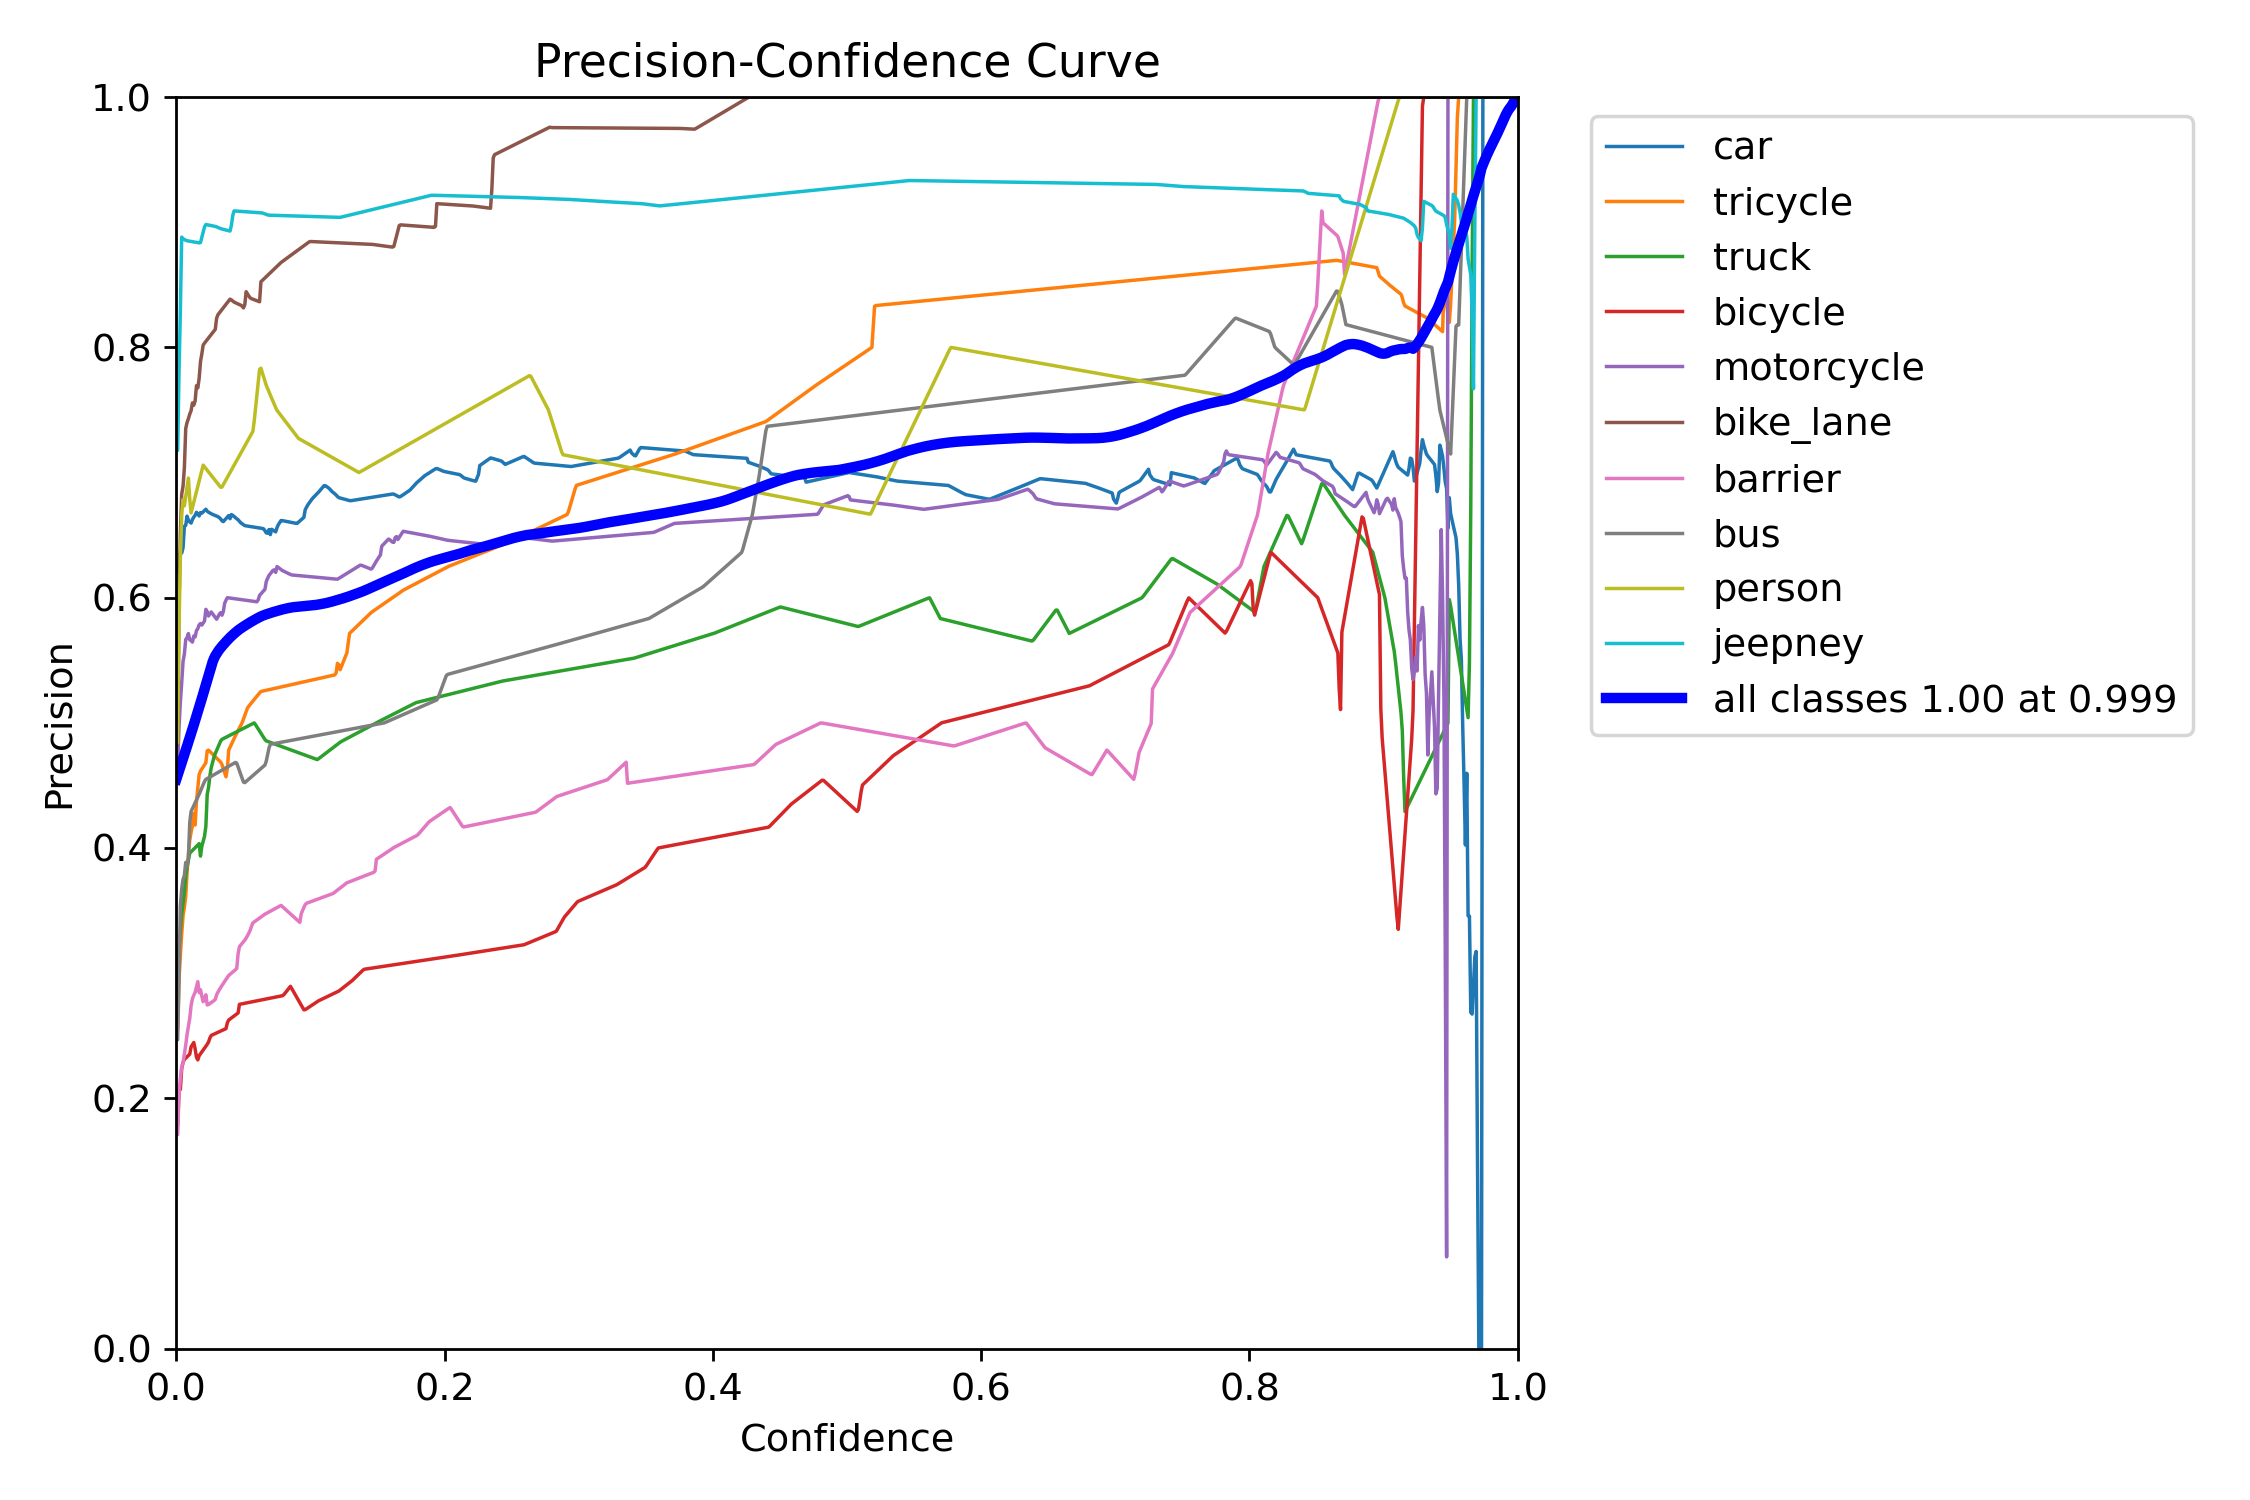
\includegraphics[width=0.75\linewidth]{figures/chapt7/section7.1/BoxP_curve.png}
    \caption{Precision-Confidence curve for bounding box detections}
    \label{fig:precision-curve-box}
\end{figure}

Generally, as confidence increases, precision also rises, indicating that the model becomes more accurate with higher certainty predictions. Notably, classes like \texttt{bike\_lane} and \texttt{jeepney} maintain consistently high precision even at lower confidence thresholds, while classes like \texttt{barrier} and \texttt{bicycle} exhibit lower precision throughout--with examples shown in Figure~\ref{fig:precision-box-imgs}.

\begin{figure}[H]
    \centering
    % Row 1
    \begin{subfigure}[b]{0.45\textwidth}
        \centering
        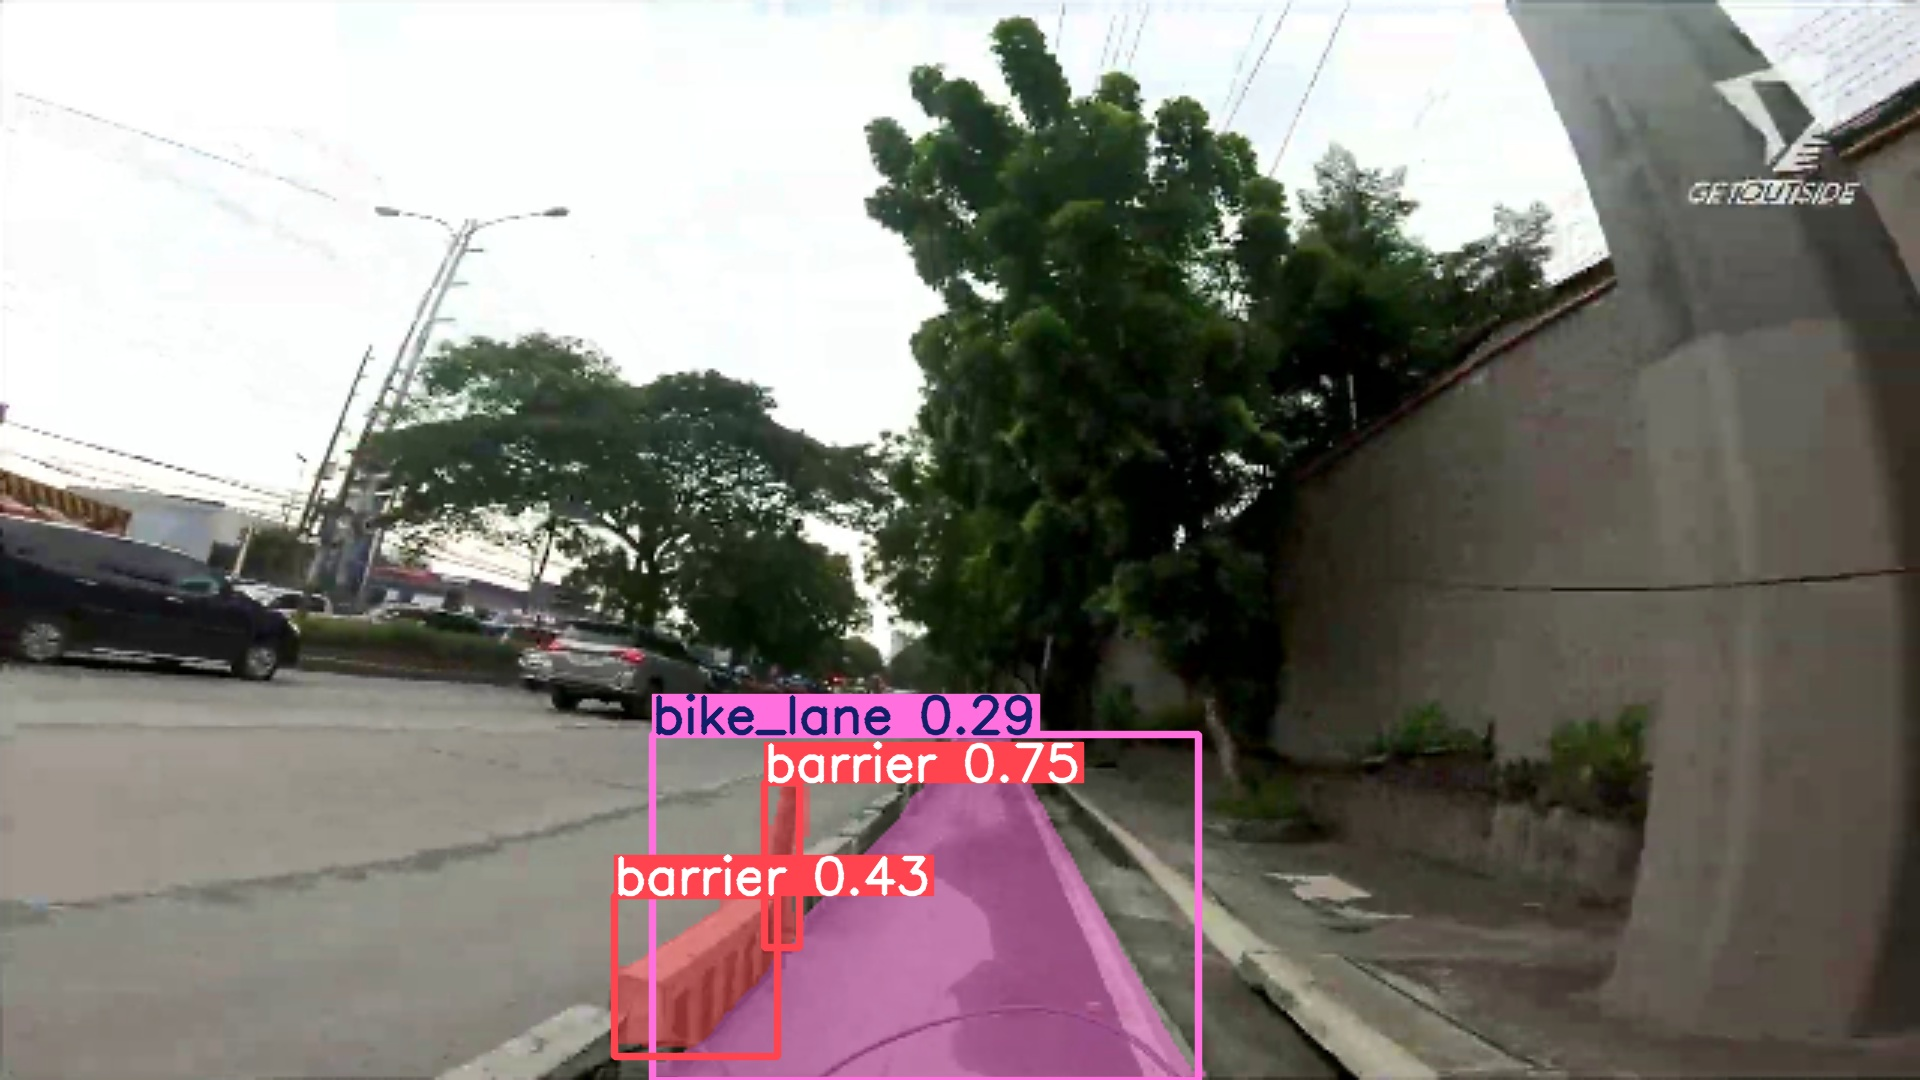
\includegraphics[width=\linewidth]{figures/chapt7/section7.1/inferred_frame_0061.jpg}
        \caption{\texttt{barrier} (mixed precision scores) and \texttt{bike\_lane} (low score) classification}
    \end{subfigure}
    \hfill
    \begin{subfigure}[b]{0.45\textwidth}
        \centering
        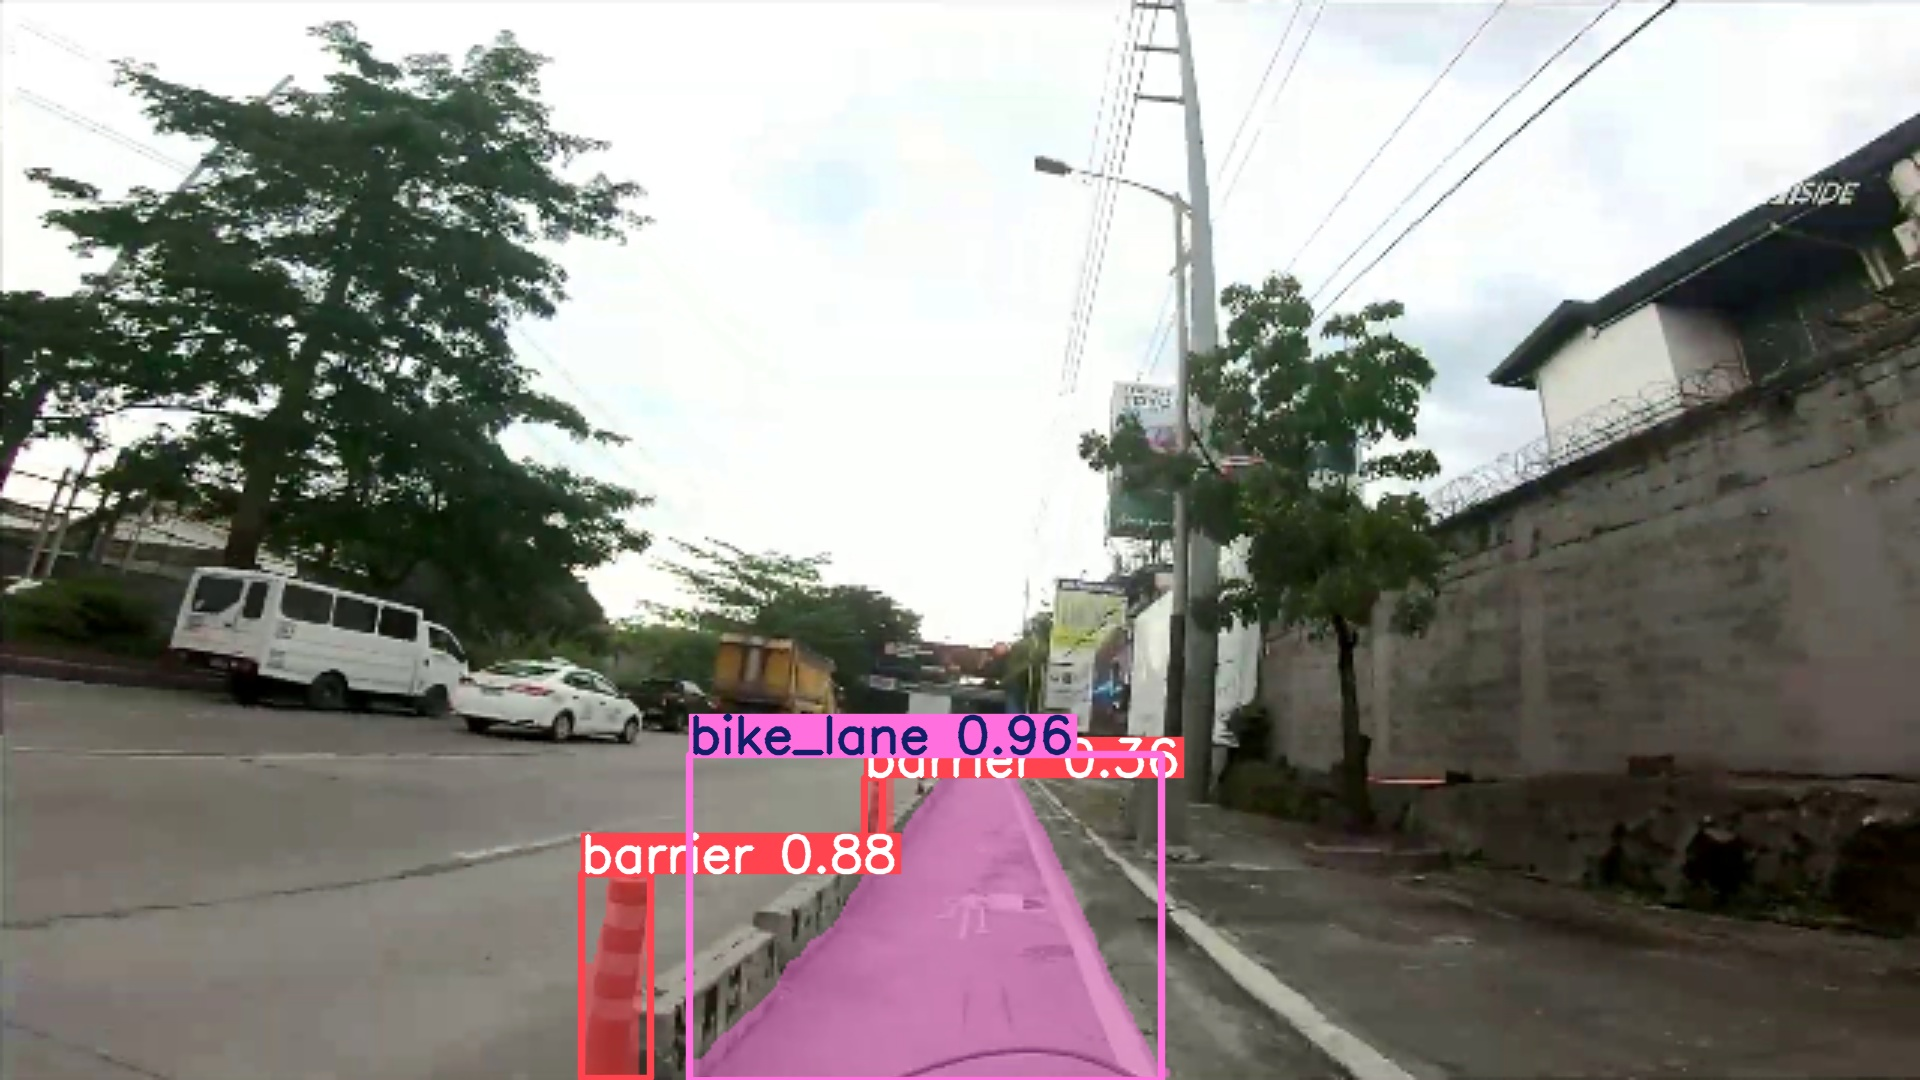
\includegraphics[width=\linewidth]{figures/chapt7/section7.1/inferred_frame_0075.jpg}
        \caption{\texttt{barrier} (mixed precision scores) and \texttt{bike\_lane} (high score) classification}
    \end{subfigure}

    \vspace{0.5cm} % space between rows

    % Row 2
    \begin{subfigure}[b]{0.45\textwidth}
        \centering
        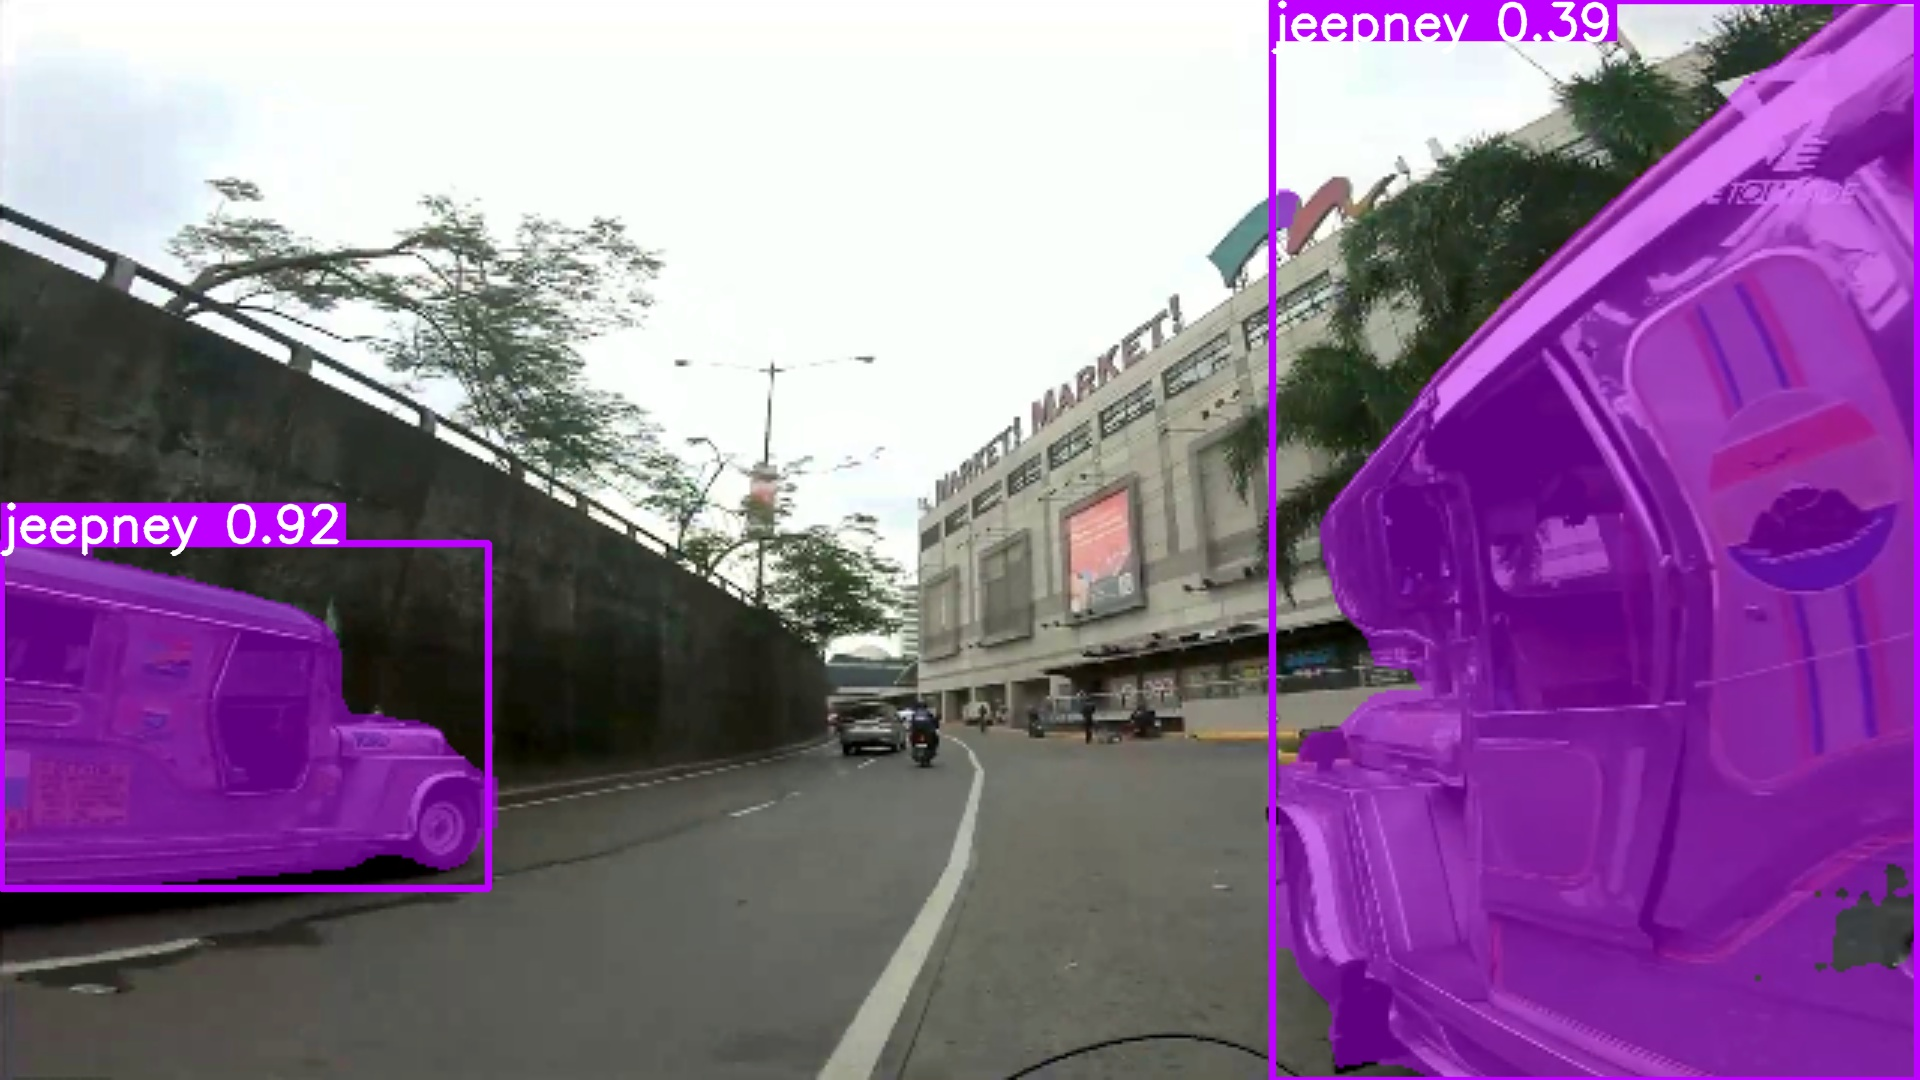
\includegraphics[width=\linewidth]{figures/chapt7/section7.1/inferred_frame_0174.jpg}
        \caption{Mixed classification scores for \texttt{jeepney} instances (high and low scores)}
    \end{subfigure}
    \hfill
    \begin{subfigure}[b]{0.45\textwidth}
        \centering
        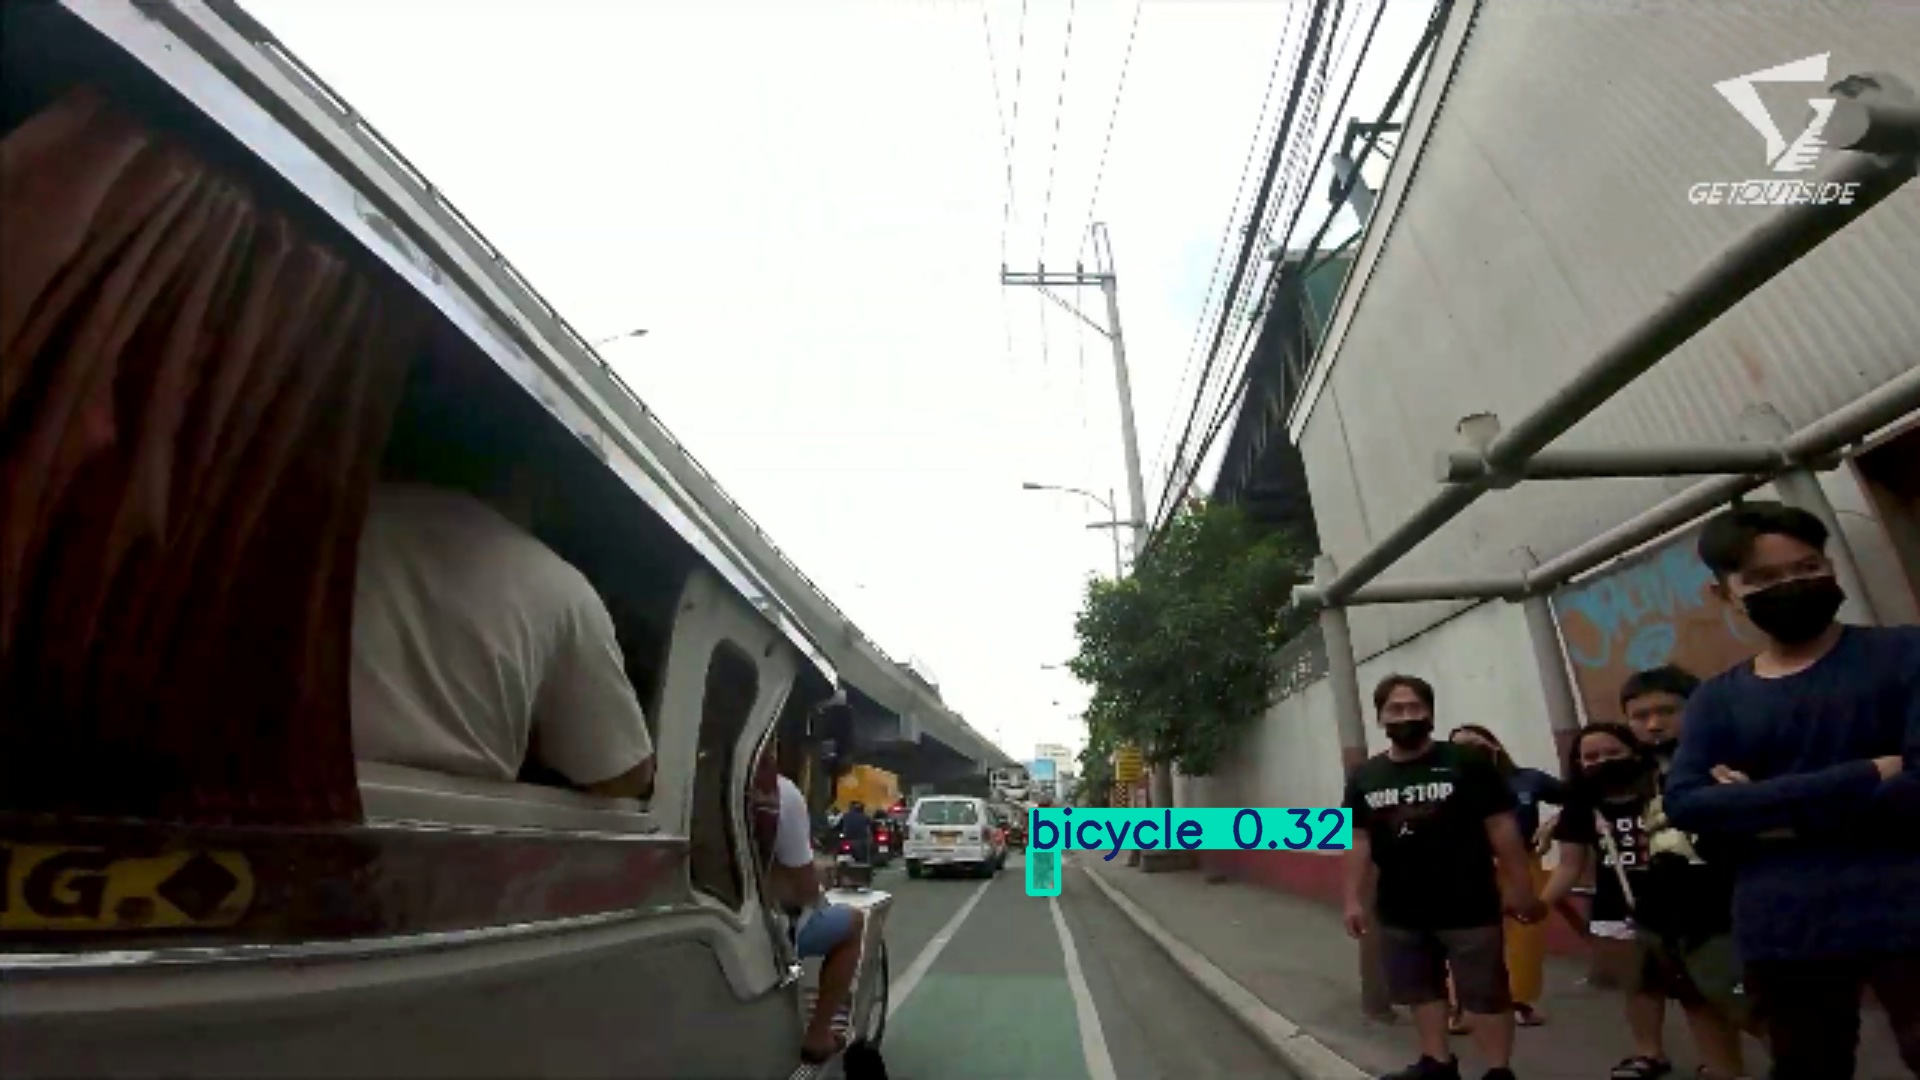
\includegraphics[width=\linewidth]{figures/chapt7/section7.1/inferred_frame_0107.jpg}
        \caption{Low precision score on \texttt{bicycle} classification}
    \end{subfigure}

    \caption{Sample classifications with varying precision scores}
    \label{fig:precision-box-imgs}
\end{figure}

The thick blue curve represents the macro-average across all classes, peaking at a precision of 1.00 when the confidence threshold reaches approximately 0.999. This suggests that the model is highly reliable at very high confidence scores, making it suitable for applications requiring high-precision predictions, albeit possibly at the cost of recall.

This behavior can be attributed to several factors. First, the rise in precision with increasing confidence is expected because the model assigns higher confidence scores to predictions it deems more certain—likely due to strong, unambiguous visual features or sufficient representation in the training data. Classes such as \texttt{bike\_lane} and \texttt{jeepney} have more distinct and consistent visual characteristics, as well as sufficient training examples, allowing the model to learn strong distinctive features that lead to confident and accurate predictions. In contrast, classes like \texttt{barrier} and \texttt{bicycle} have more visual variability, ambiguous boundaries, and fewer annotated instances in the dataset, resulting in less confident and more error-prone predictions. Furthermore, the precision peaking near a confidence score of 0.999 reflects the model's calibration—only a few predictions reach such a high confidence, but when they do, they are highly likely to be correct. This trade-off is typical in detection models like YOLOv11, where pushing for high precision at extreme confidence levels inherently reduces the number of detections, but ensures that those retained predictions are almost certainly correct.

\subsubsection{Mask}
The Precision-Confidence Curve, seen in Figure~\ref{fig:precision-curve-mask}, shows that precision generally increases with higher confidence thresholds in most classes, with the overall precision (bold blue) reaching a perfect score of 1.00 with a confidence of 0.999.

\begin{figure}[H]
    \centering
    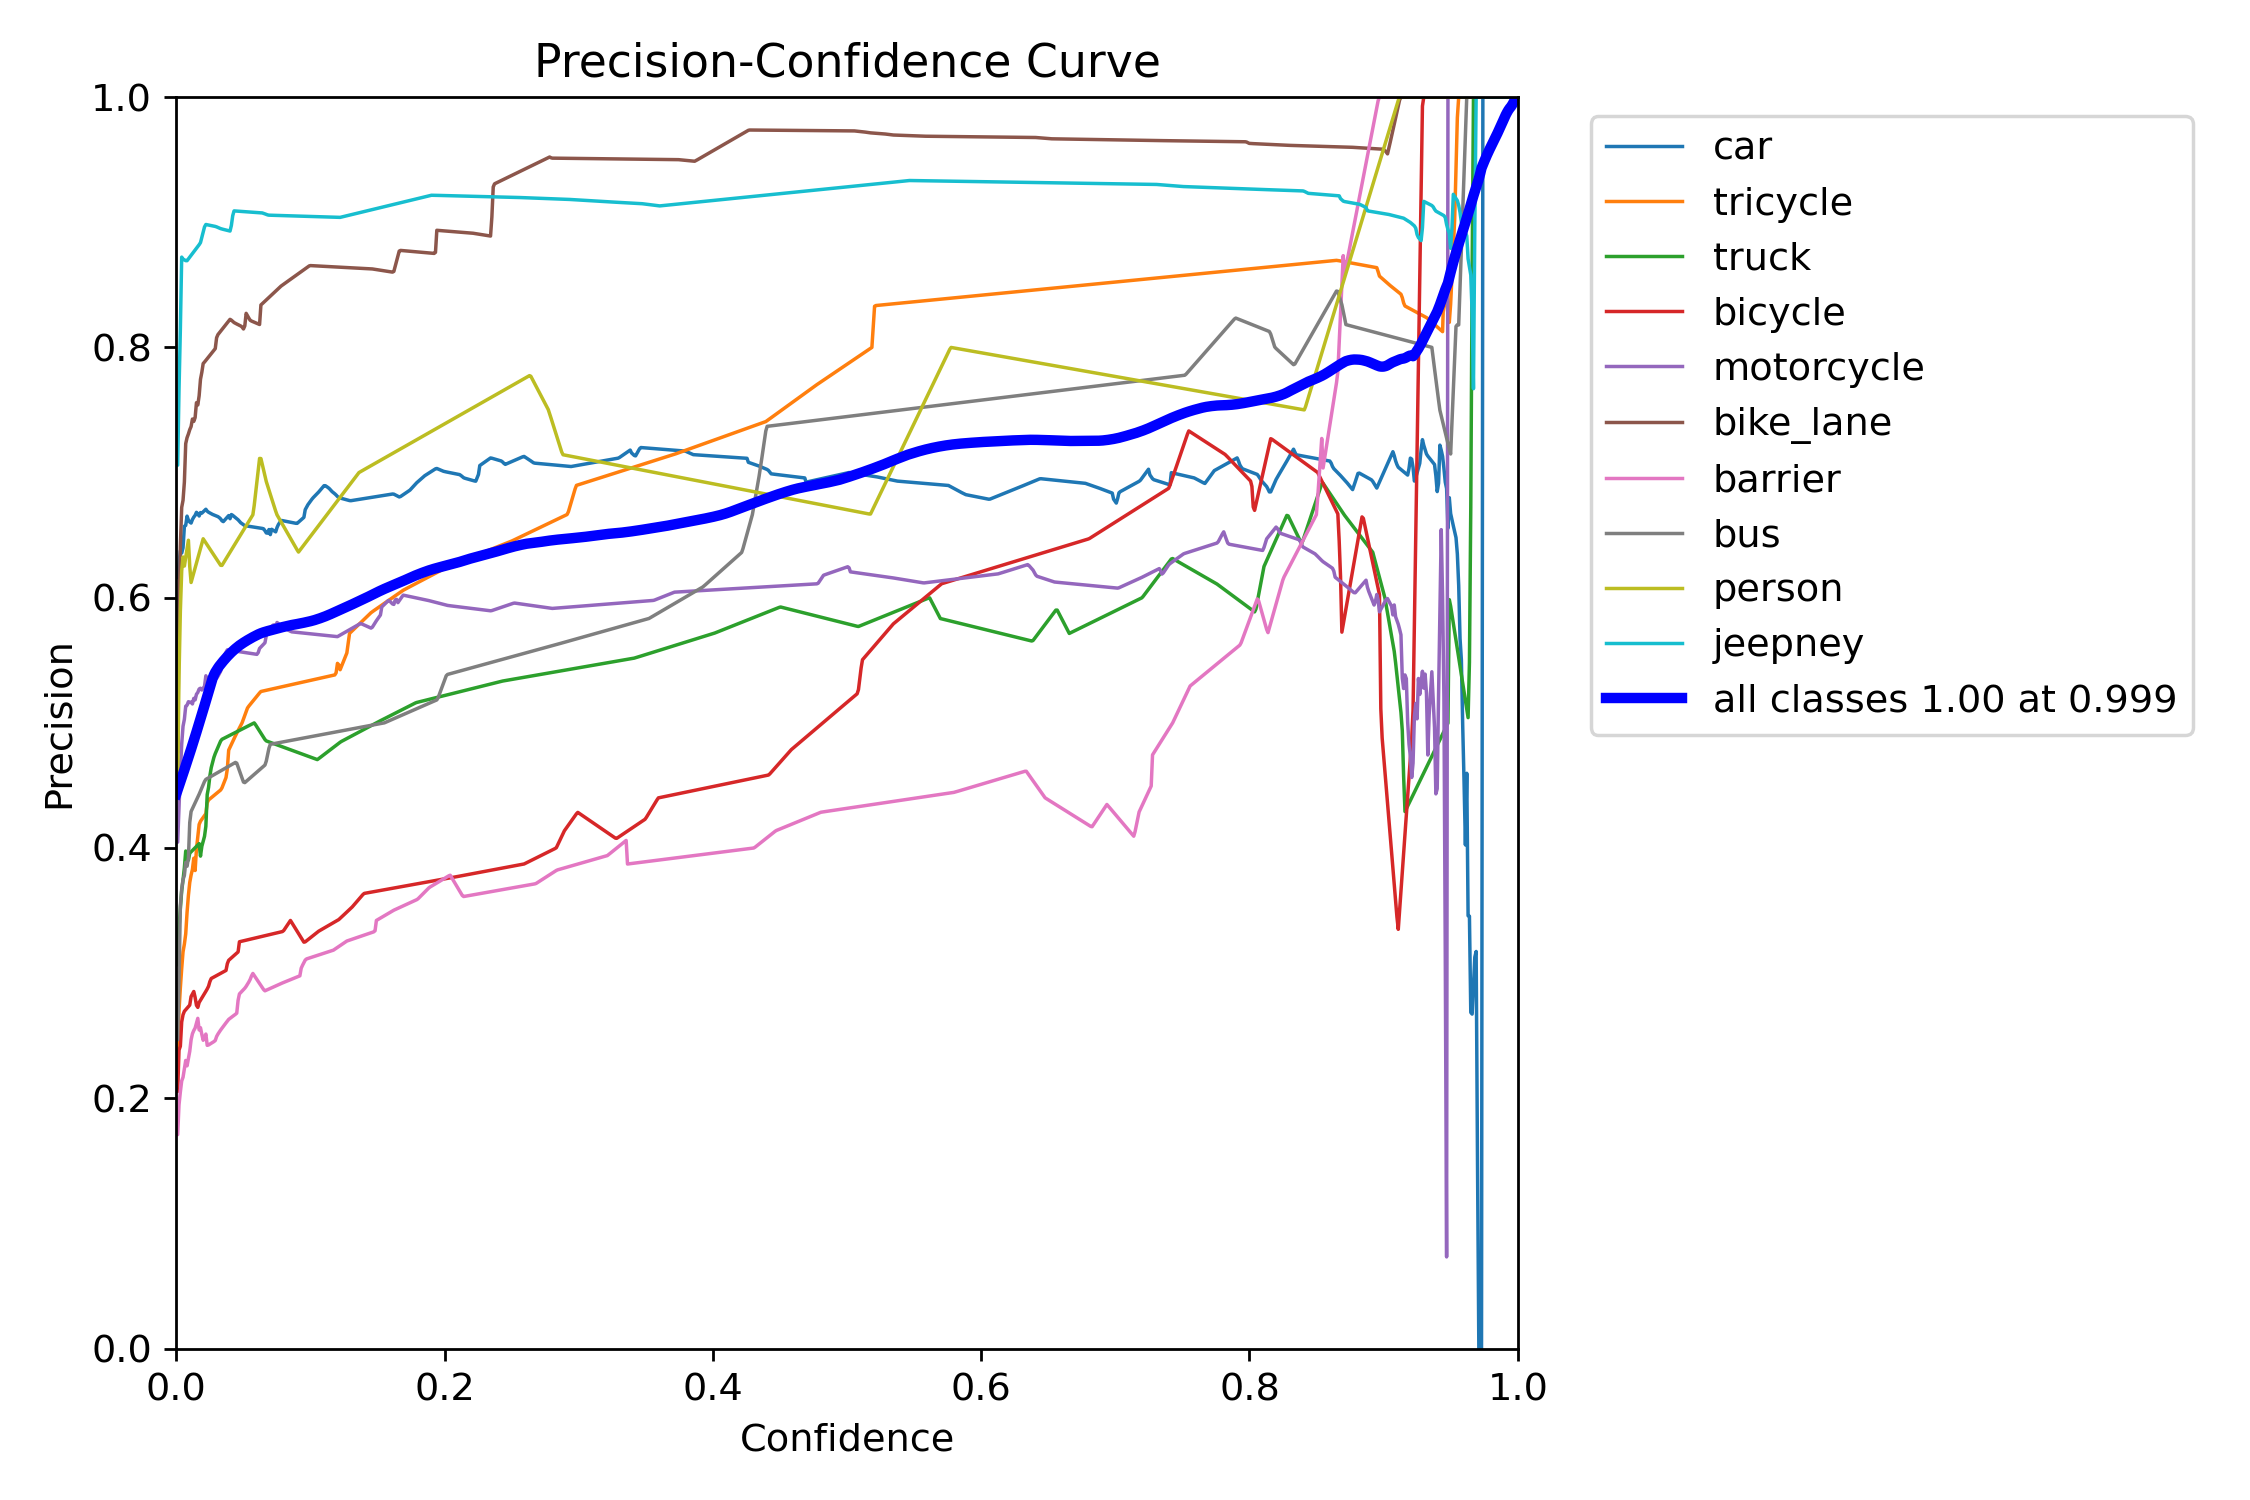
\includegraphics[width=0.75\linewidth]{figures/chapt7/section7.1/MaskP_curve.png}
    \caption{Precision-Confidence Curve for Mask Segmentation}
    \label{fig:precision-curve-mask}
\end{figure}

Classes such as \texttt{bike\_lane}, \texttt{jeepney}, and \texttt{bus} maintain high precision (often above 0.85) even at lower confidence thresholds, indicating the model's strong ability to avoid false positives for these classes. In contrast, classes like \texttt{barrier}, \texttt{bicycle}, and \texttt{person} show lower and more unstable precision throughout, suggesting more frequent misclassifications--with examples shown in Figure~\ref{fig:precision-mask-imgs}. 

\begin{figure}[H]
    \centering
    % Row 1
    \begin{subfigure}[b]{0.45\textwidth}
        \centering
        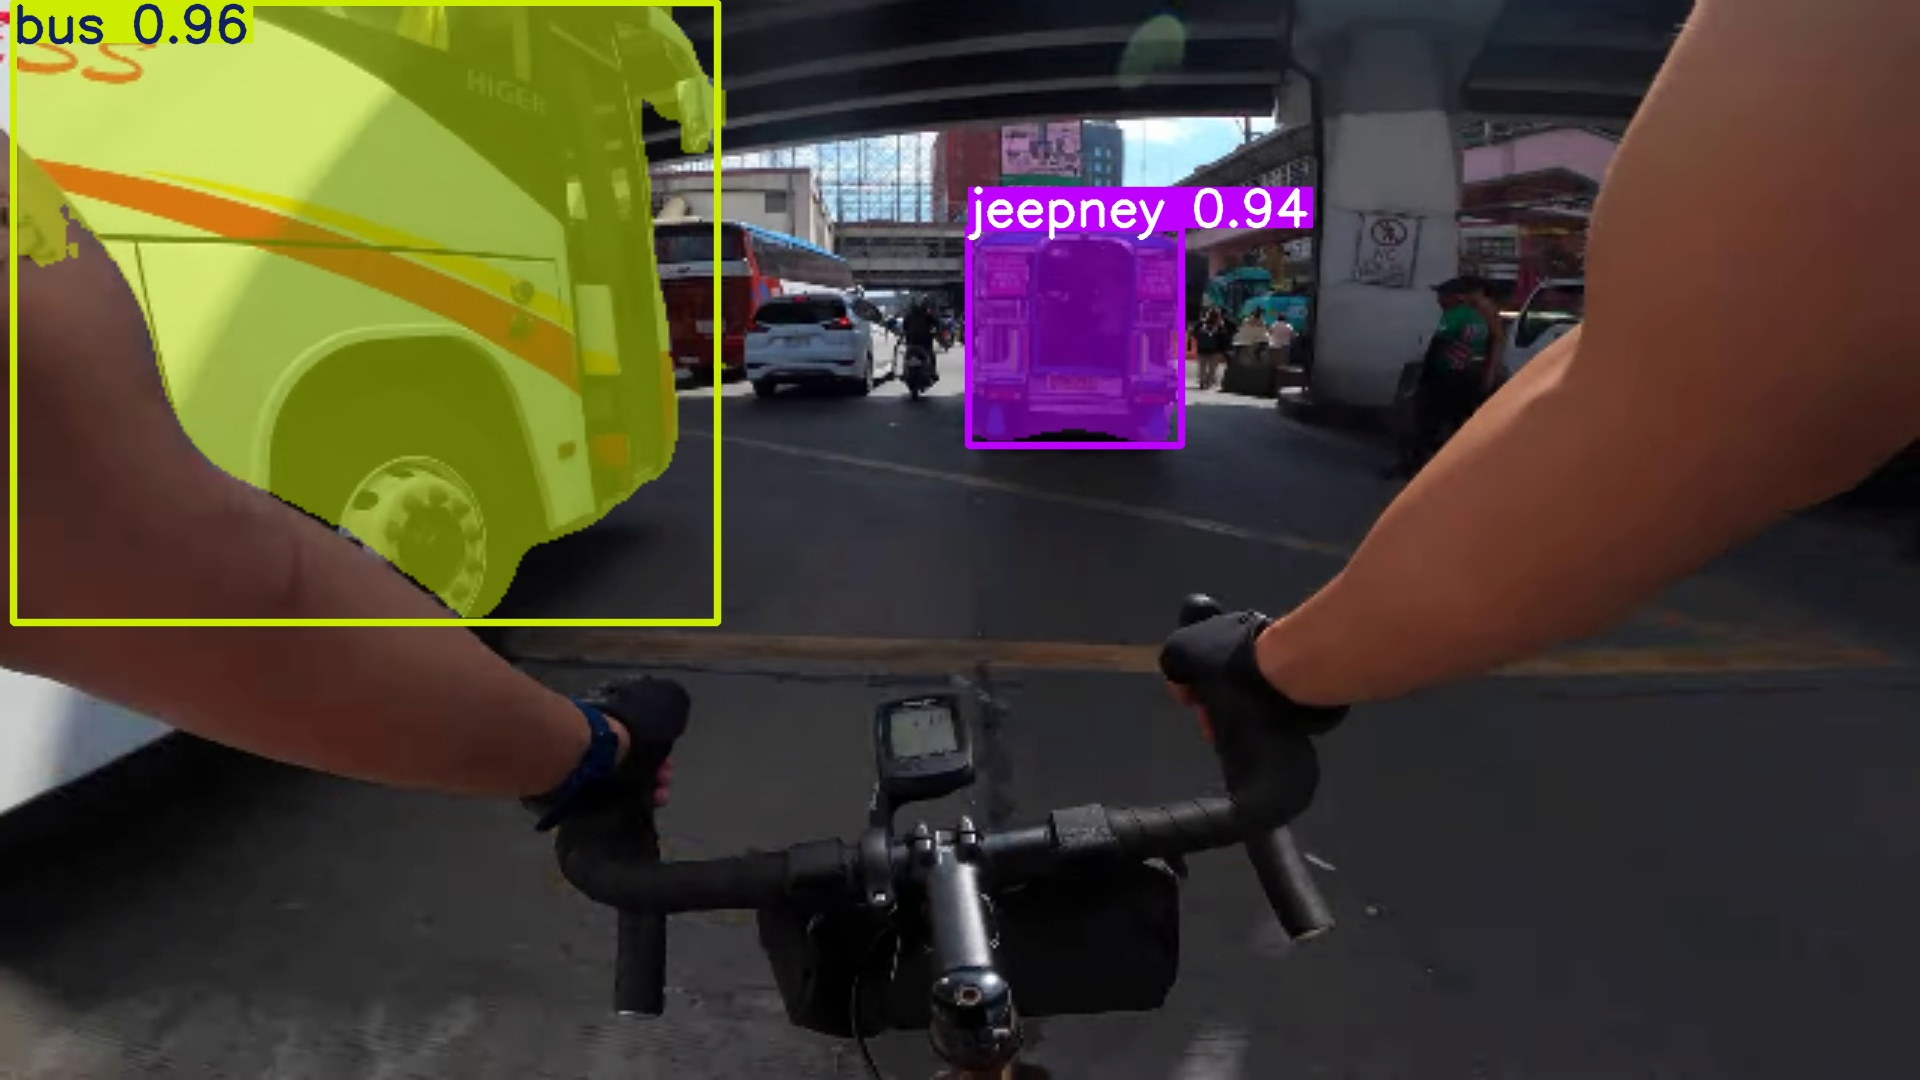
\includegraphics[width=\linewidth]{figures/chapt7/section7.1/inferred_frame_0030.jpg}
        \caption{\texttt{bus} and \texttt{jeepney} classification with high precision}
    \end{subfigure}
    \hfill
    \begin{subfigure}[b]{0.45\textwidth}
        \centering
        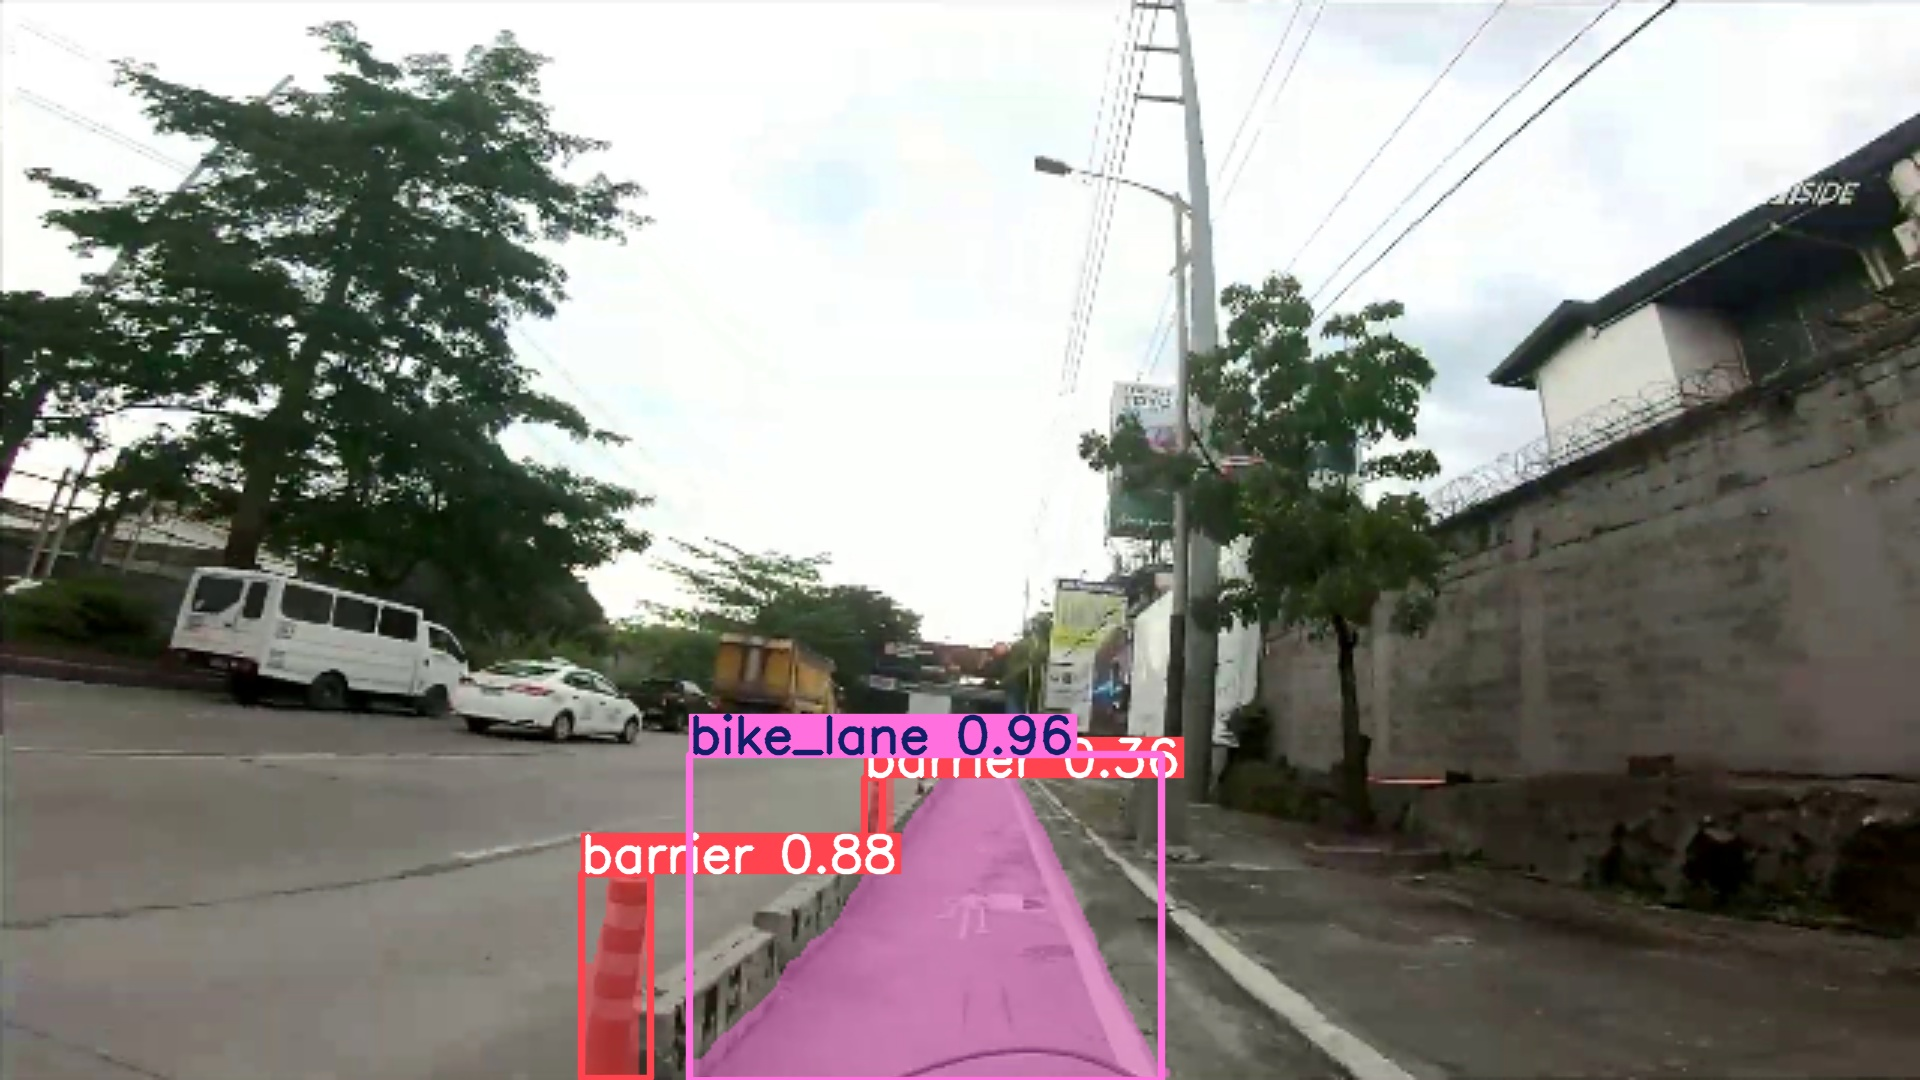
\includegraphics[width=\linewidth]{figures/chapt7/section7.1/inferred_frame_0075.jpg}
        \caption{\texttt{bus} and \texttt{bike\_lane} classification with high precision}
    \end{subfigure}

    \vspace{0.5cm} % space between rows

    % Row 2
    \begin{subfigure}[b]{0.45\textwidth}
        \centering
        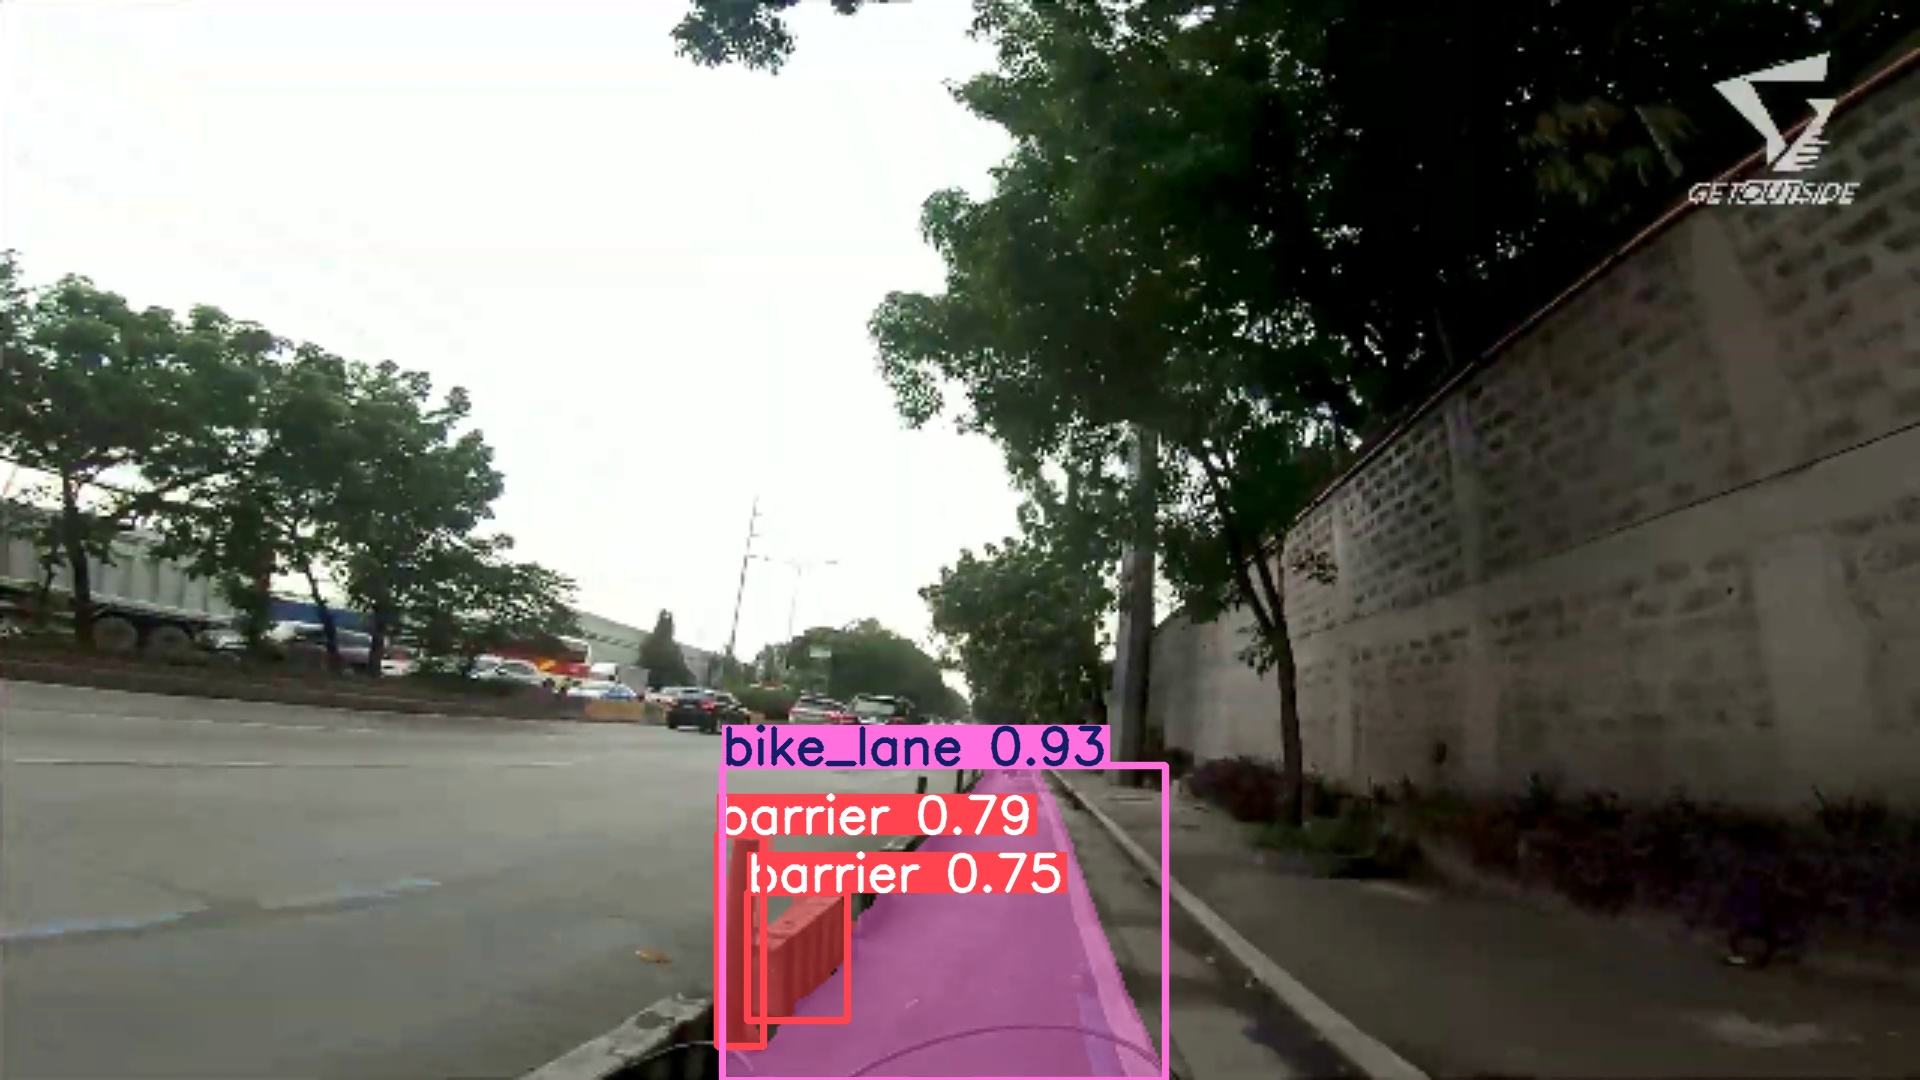
\includegraphics[width=\linewidth]{figures/chapt7/section7.1/inferred_frame_0063.jpg}
        \caption{\texttt{barrier} classification on bollard and concrete barriers with varying scores}
    \end{subfigure}
    \hfill
    \begin{subfigure}[b]{0.45\textwidth}
        \centering
        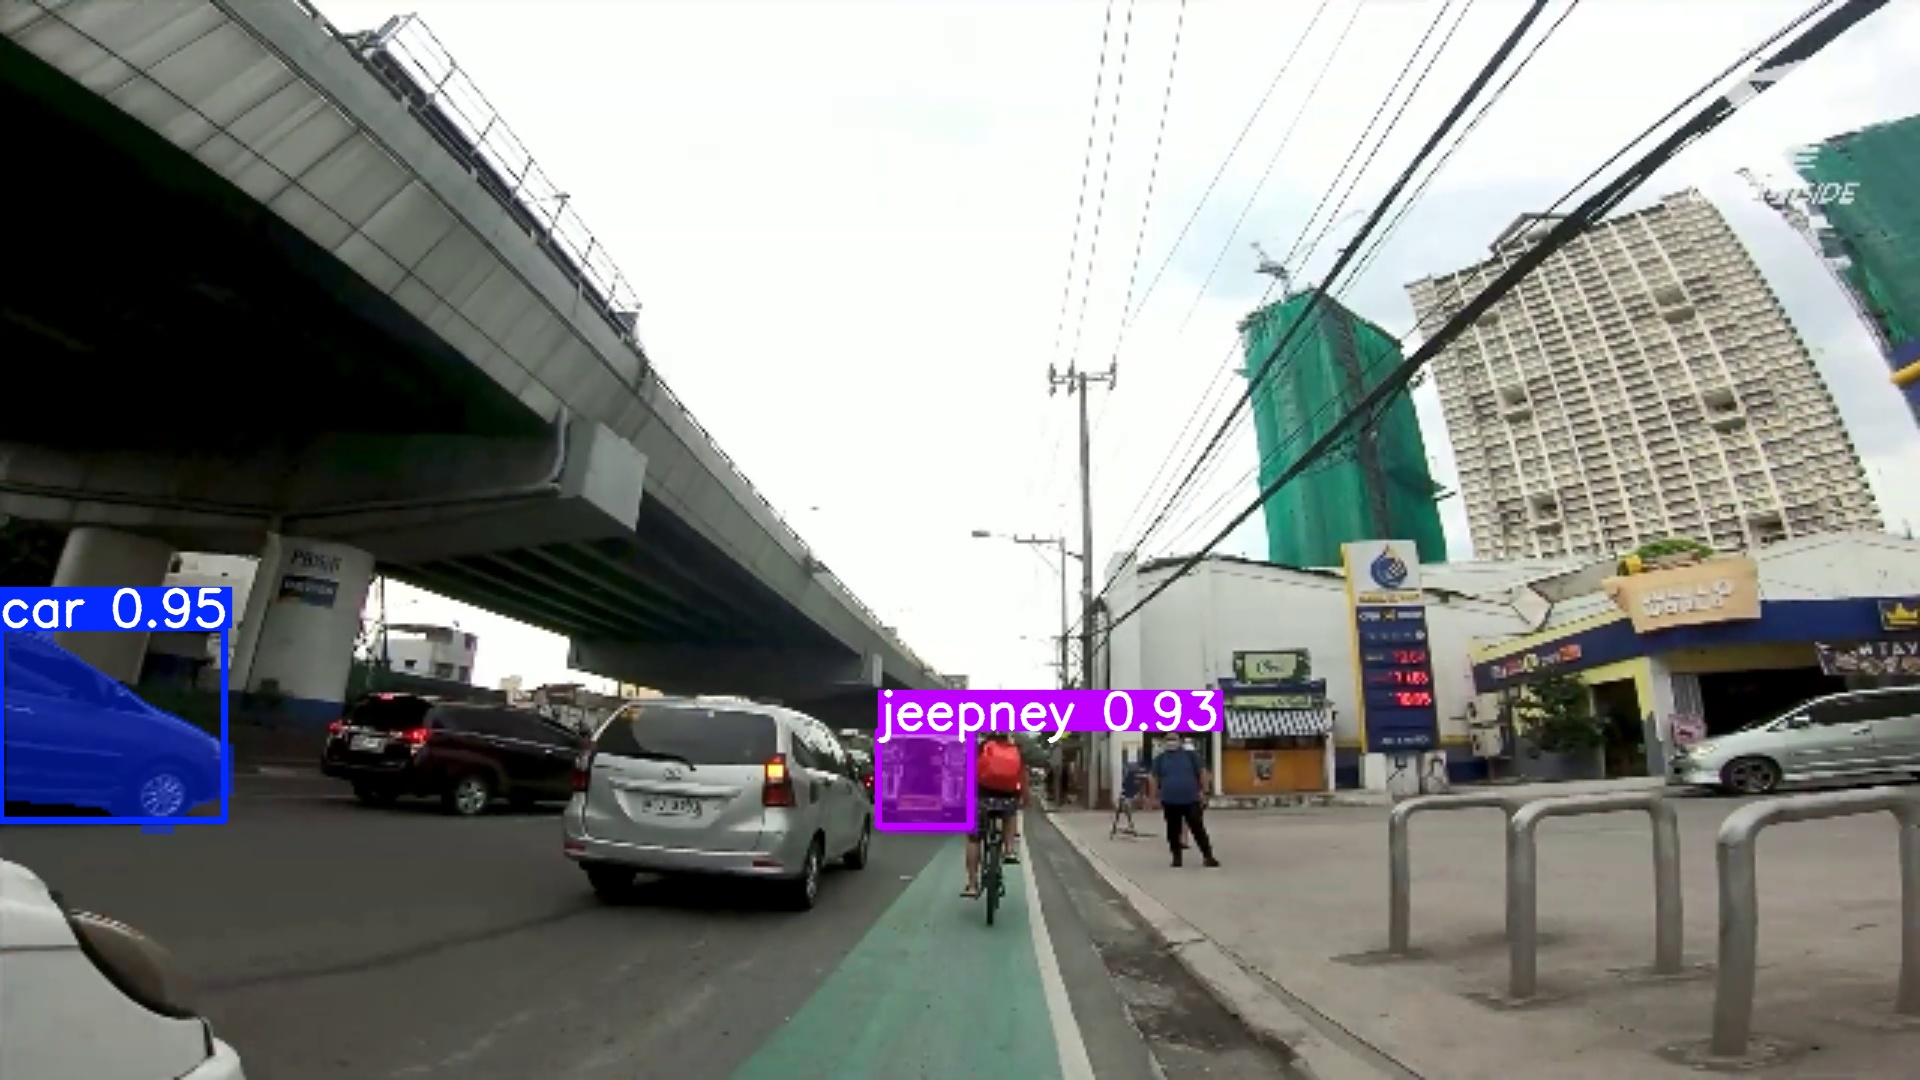
\includegraphics[width=\linewidth]{figures/chapt7/section7.1/inferred_frame_0105.jpg}
        \caption{Missed classification (undefined precision) on \texttt{bicycle} and \texttt{person} instances}
    \end{subfigure}

    \caption{Sample classifications with varying precision scores}
    \label{fig:precision-mask-imgs}
\end{figure}

The sharp spike in overall precision near the highest confidence values implies that the model becomes extremely conservative at these thresholds, favoring fewer but highly accurate predictions. This precision behavior is desirable for applications where false positives must be minimized, such as aggregating object presence from video frames for scene annotation, although it must be balanced with recall, which may drop steeply at these thresholds.

This trend can be explained by how the model learns to associate visual patterns with object masks across different classes. Classes like \texttt{bike\_lane}, \texttt{jeepney}, and \texttt{bus} possess strong, consistent visual cues,such as unique shapes, colors, or textures, that make them easier for the model to segment confidently and correctly, even under varying conditions. These objects may have also been overrepresented in the training set, which improved the model's capacity to learn distinctive features. On the other hand, classes such as \texttt{barrier}, \texttt{bicycle}, and \texttt{person} tend to appear in more complex scenes, have more occlusion, and exhibit greater intra-class variability. This makes segmentation more challenging and increases the likelihood of confusion with other classes, especially at lower confidence thresholds. The sudden spike in precision near a confidence of 0.999 reflects the model's internal calibration—it only assigns such high confidence to predictions it is almost certain about, likely those with clear visual separation and high feature agreement. While this behavior minimizes false positives, it also means that many correct but less confident predictions are discarded, affecting recall. Thus, the precision trend reflects both the quality of feature learning for each class and the model's conservative bias at high thresholds.

\subsection{Recall}

\subsubsection{Box}
The recall performance for bounding box predictions across different confidence thresholds is presented in Figure~\ref{fig:recall-curve-box} with the Recall-Confidence Curve. The overall recall across all classes, shown by the thick blue line, peaks at approximately 0.33 at the lowest confidence threshold, suggesting that only about one-third of true objects are detected when accepting all predictions regardless of confidence. As confidence increases, recall steadily drops across all classes, indicating that higher thresholds lead to more missed detections.

\begin{figure}[H]
    \centering
    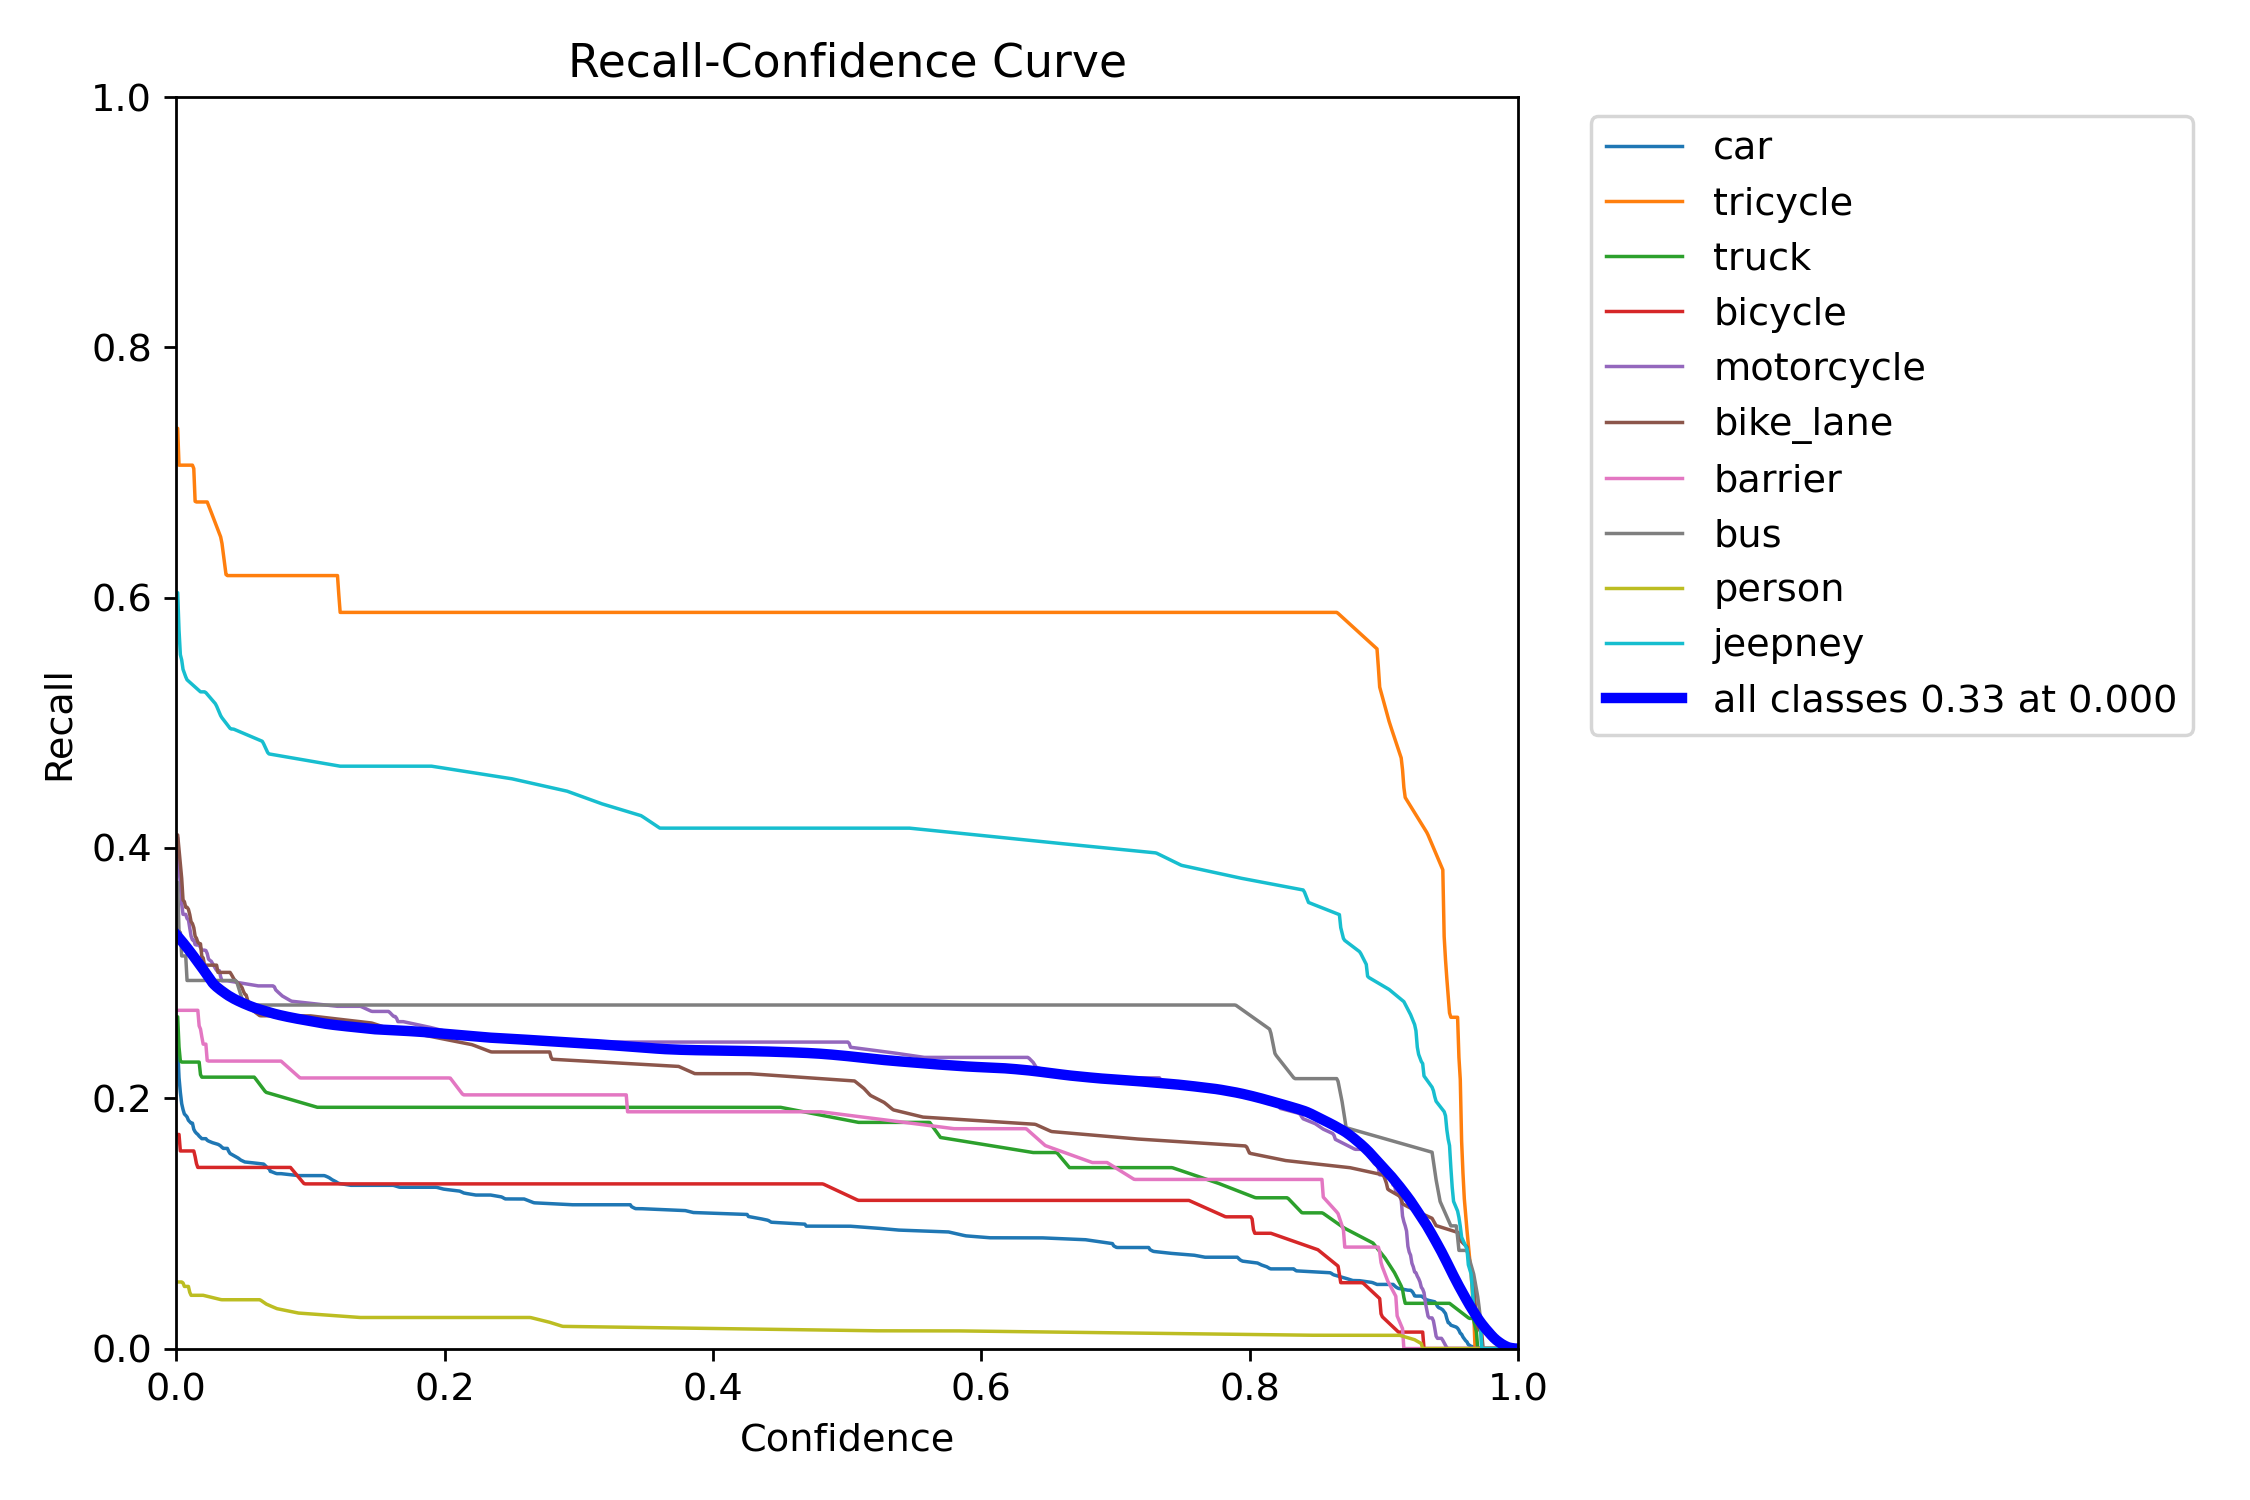
\includegraphics[width=0.75\linewidth]{figures/chapt7/section7.1/BoxR_curve.png}
    \caption{Recall-Confidence Curve for Bounding Box Predictions}
    \label{fig:recall-curve-box}
\end{figure}

Class-specific performance varies significantly: \texttt{tricycle} and \texttt{jeepney} stand out with the highest recall values, especially at lower thresholds, while classes like \texttt{person} and \texttt{bicycle} maintain consistently low recall, likely due to fewer detections or higher localization difficulty. The flat regions followed by steep drops imply that the model is making only a limited number of confident detections for each class. Overall, while some classes perform decently in terms of recall, the model appears to favor precision, with room for improvement in overall object coverage.

This behavior can be explained by several underlying factors related to the model's training dynamics and class-specific characteristics. First, the low peak recall at minimal confidence suggests that the model either produces a limited number of detections overall or is overly conservative in generating proposals. YOLOv11, while optimized for speed and precision, may underproduce low-confidence predictions—especially for smaller or less visually distinct objects—resulting in missed detections even when all outputs are considered. The declining recall with increasing confidence reflects the model's internal trade-off: it filters out uncertain predictions to increase precision, but in doing so, it also discards potentially correct predictions that fall below the threshold.

High-recall classes like \texttt{tricycle} and \texttt{jeepney} benefit from clearer visual features or greater representation in the training dataset, which enabled the model to consistently detect them even at lower confidences. These classes also appeared in less cluttered contexts or had larger object sizes, improving localization accuracy. In contrast, classes such as \texttt{person} and \texttt{bicycle} often appear in more complex, occluded, or densely populated scenes, making them harder to detect. Their smaller size, high variability in appearance, and possible underrepresentation in the training data contribute to low recall. Examples of these cases are illustrated below in Figure~\ref{fig:recall-box-imgs}.

\begin{figure}[H]
    \centering
    % Row 1
    \begin{subfigure}[b]{0.45\textwidth}
        \centering
        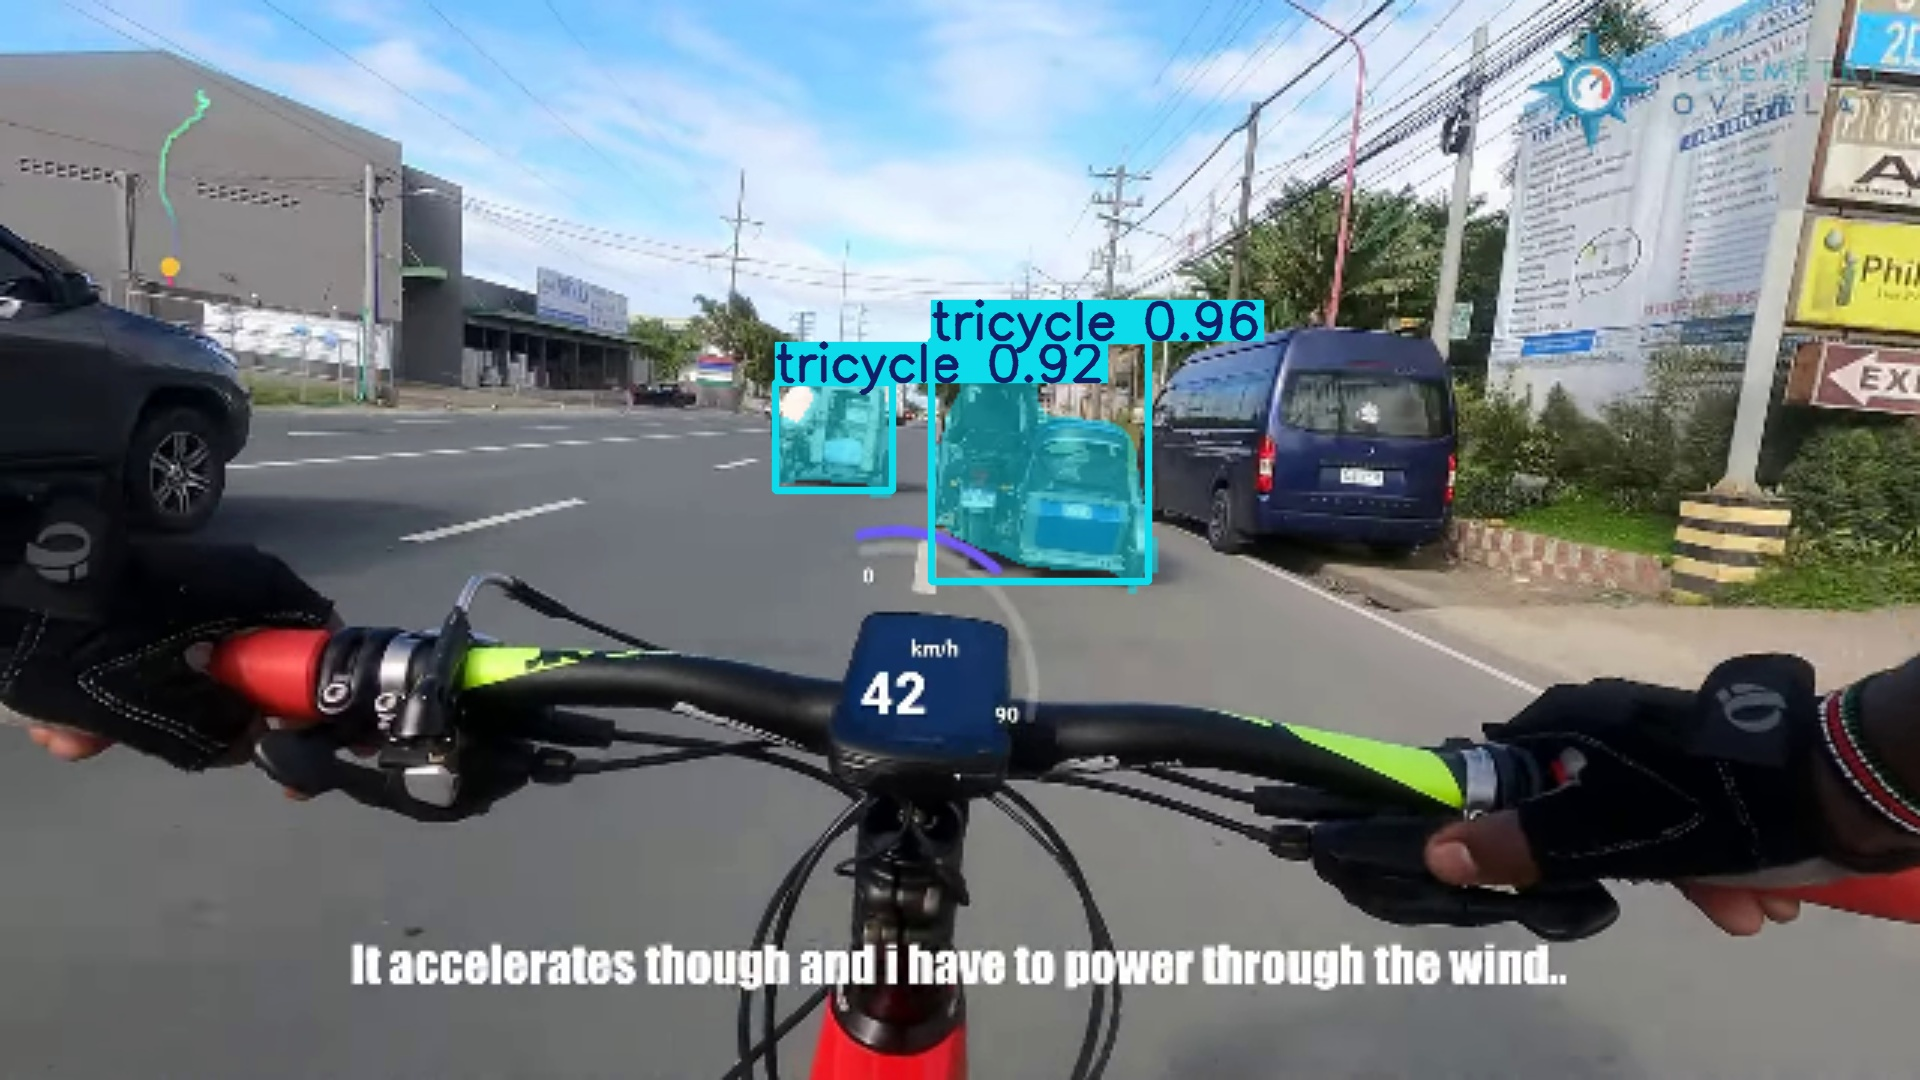
\includegraphics[width=\linewidth]{figures/chapt7/section7.1/inferred_frame_0003.jpg}
        \caption{\texttt{tricycle} instances true-positive classification}
    \end{subfigure}
    \hfill
    \begin{subfigure}[b]{0.45\textwidth}
        \centering
        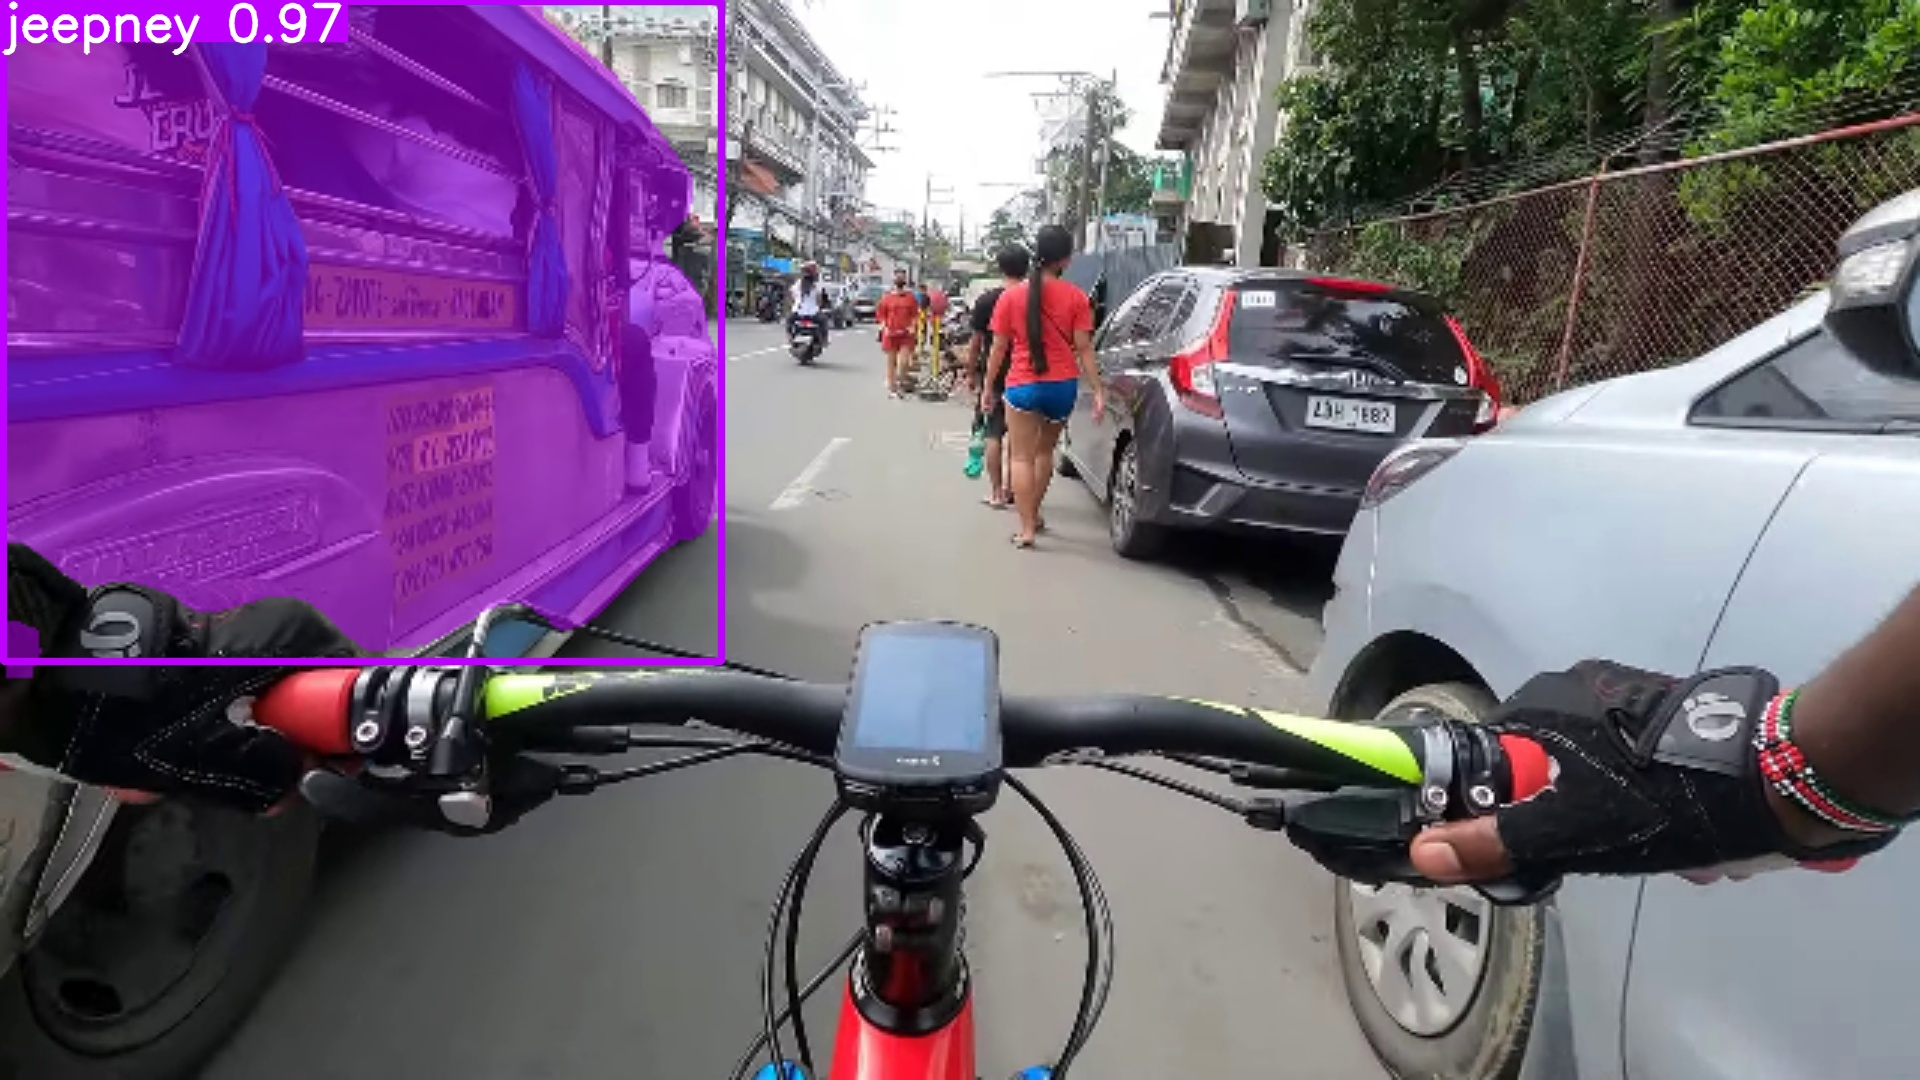
\includegraphics[width=\linewidth]{figures/chapt7/section7.1/inferred_frame_0025.jpg}
        \caption{\texttt{jeepney} instance true-positive classification}
    \end{subfigure}

    \vspace{0.5cm} % space between rows

    % Row 2
    \begin{subfigure}[b]{0.45\textwidth}
        \centering
        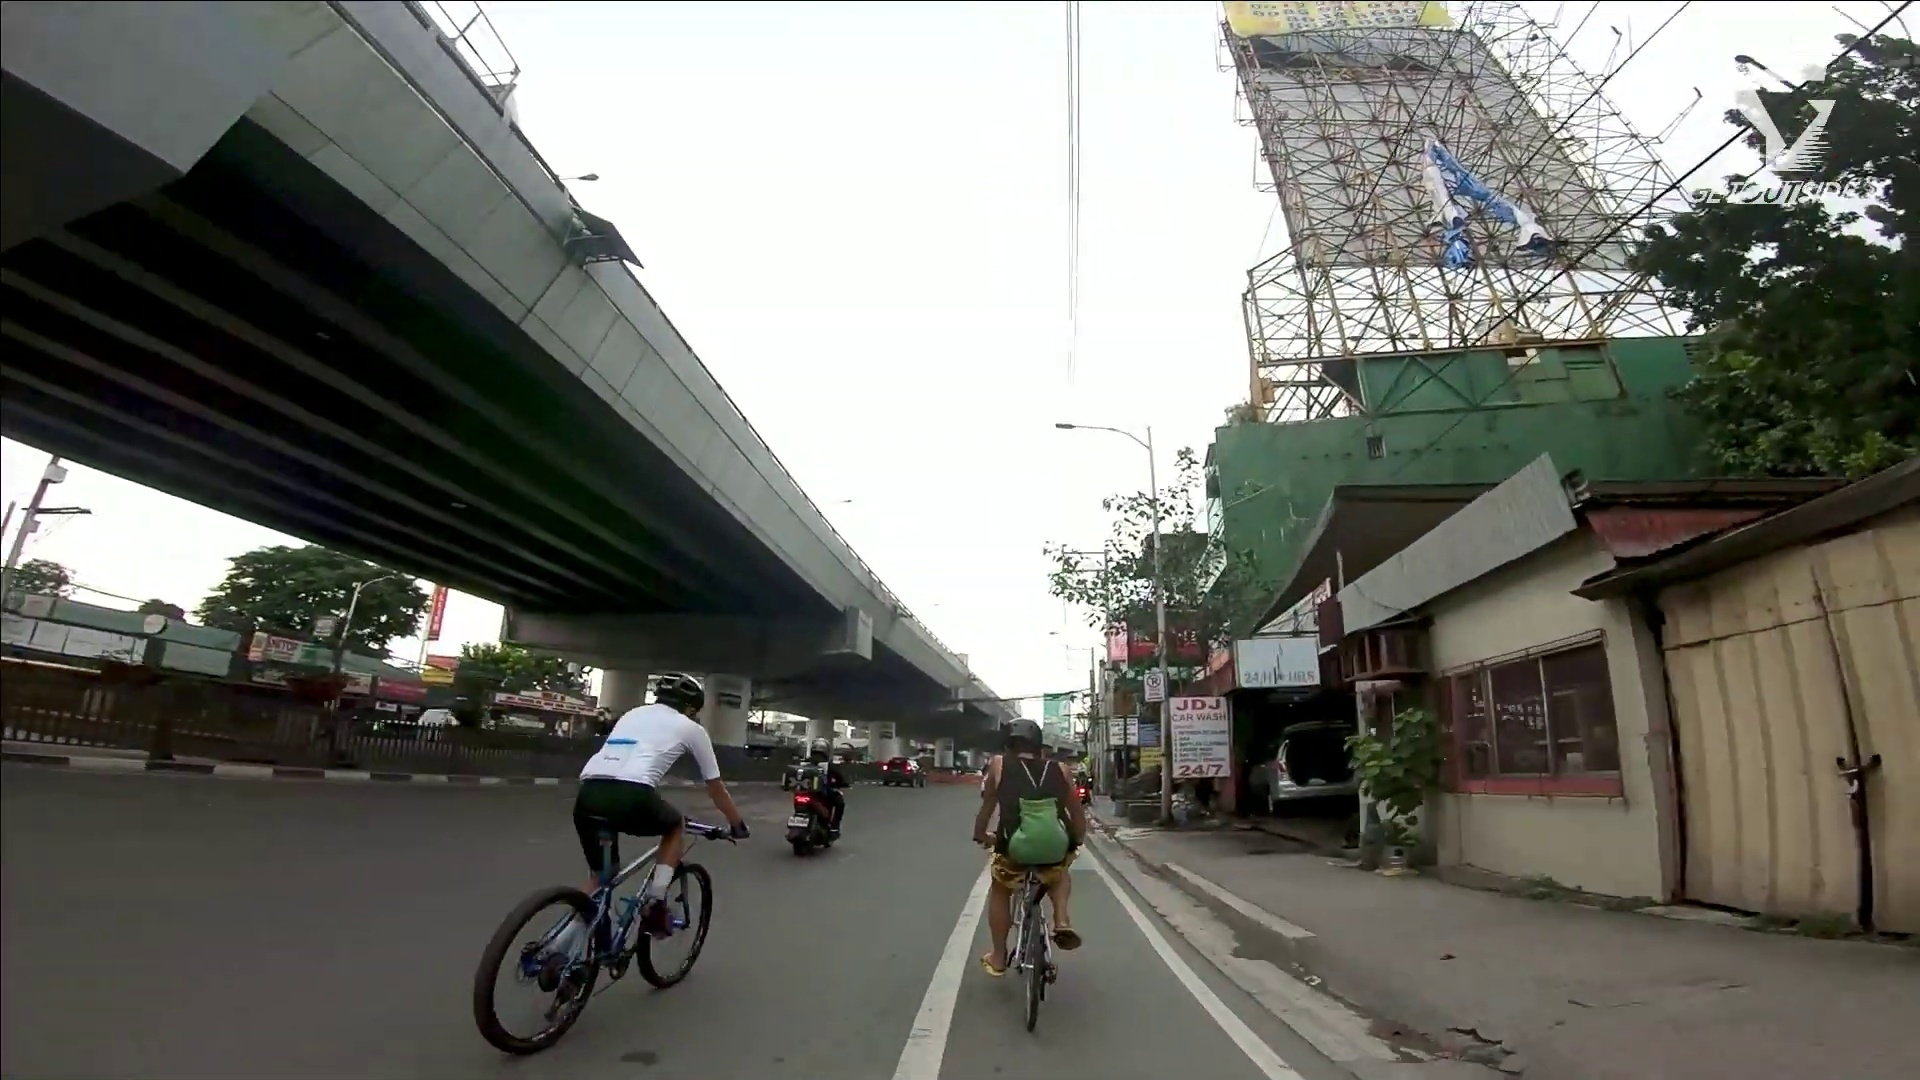
\includegraphics[width=\linewidth]{figures/chapt7/section7.1/inferred_frame_0099.jpg}
        \caption{\texttt{bicycle} instances false-negative classification}
    \end{subfigure}
    \hfill
    \begin{subfigure}[b]{0.45\textwidth}
        \centering
        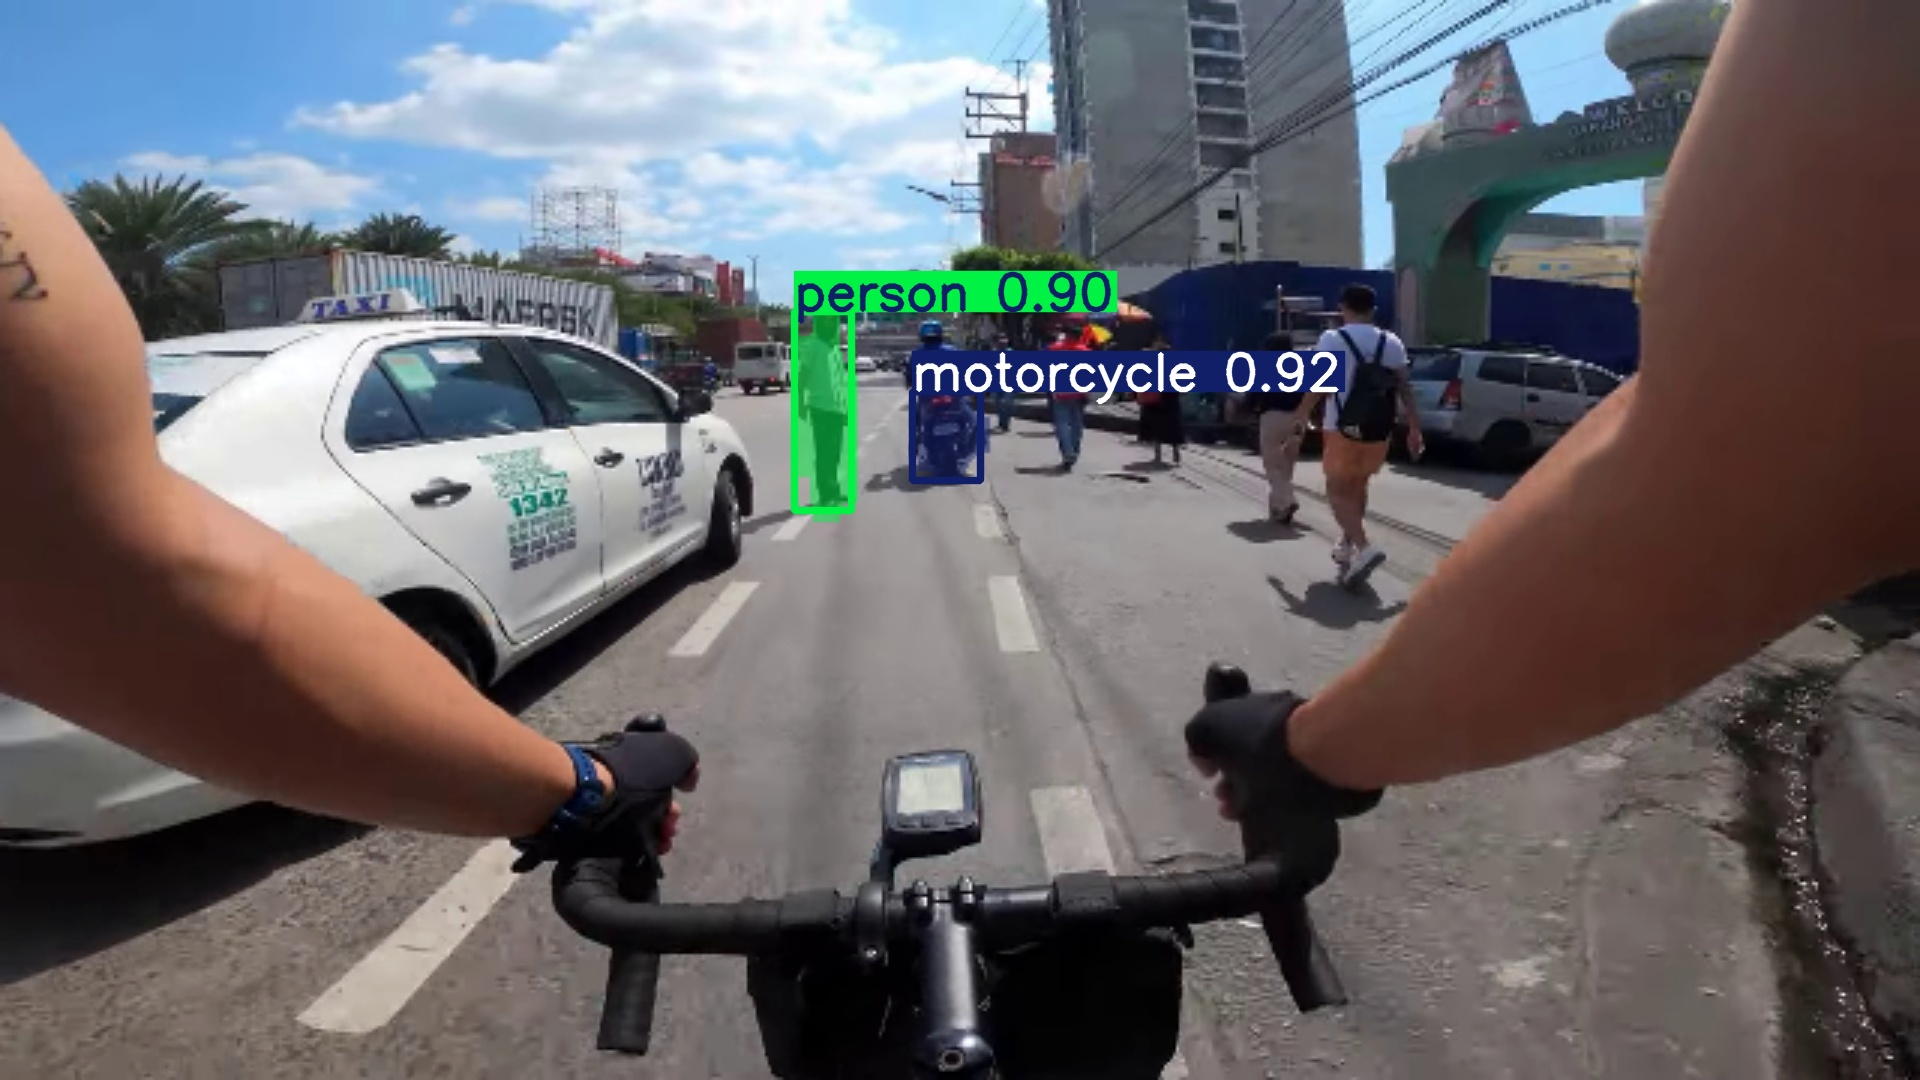
\includegraphics[width=\linewidth]{figures/chapt7/section7.1/inferred_frame_0019.jpg}
        \caption{\texttt{person} instances true-positive and false-negative classification}
    \end{subfigure}

    \caption{Sample true positive and false negative classifications}
    \label{fig:recall-box-imgs}
\end{figure}

The flat regions in the recall curve followed by sudden drops suggest that the model rarely assigns high confidence to the predictions in these classes, pointing to a lack of strong distinctive features learned for those classes.

\subsubsection{Mask}
The Recall-Confidence Curve shown in Figure~\ref{fig:recall-curve-mask} demonstrates how recall performance for mask predictions varies across confidence thresholds for each class. The overall recall, shown by the thick blue line, peaks at 0.32 at zero confidence, meaning the model captures roughly 32\% of all ground-truth objects when including all predictions. Similar to the bounding box recall, performance drops steadily as confidence increases.The \texttt{tricycle} and \texttt{jeepney} classes again stand out with significantly higher recall (up to 0.6), suggesting that the model is particularly good at segmenting these object types. In contrast, classes such as \texttt{person}, \texttt{bicycle}, and \texttt{truck} have consistently low recall, likely due to segmentation difficulties or class imbalance. The overall curve shapes indicate the model is conservative with mask predictions, prioritizing precision, and tends to miss detections at higher confidence thresholds. This behavior highlights the need for improved recall, especially for safety-critical or frequently occurring object classes.

\begin{figure}[H]
    \centering
    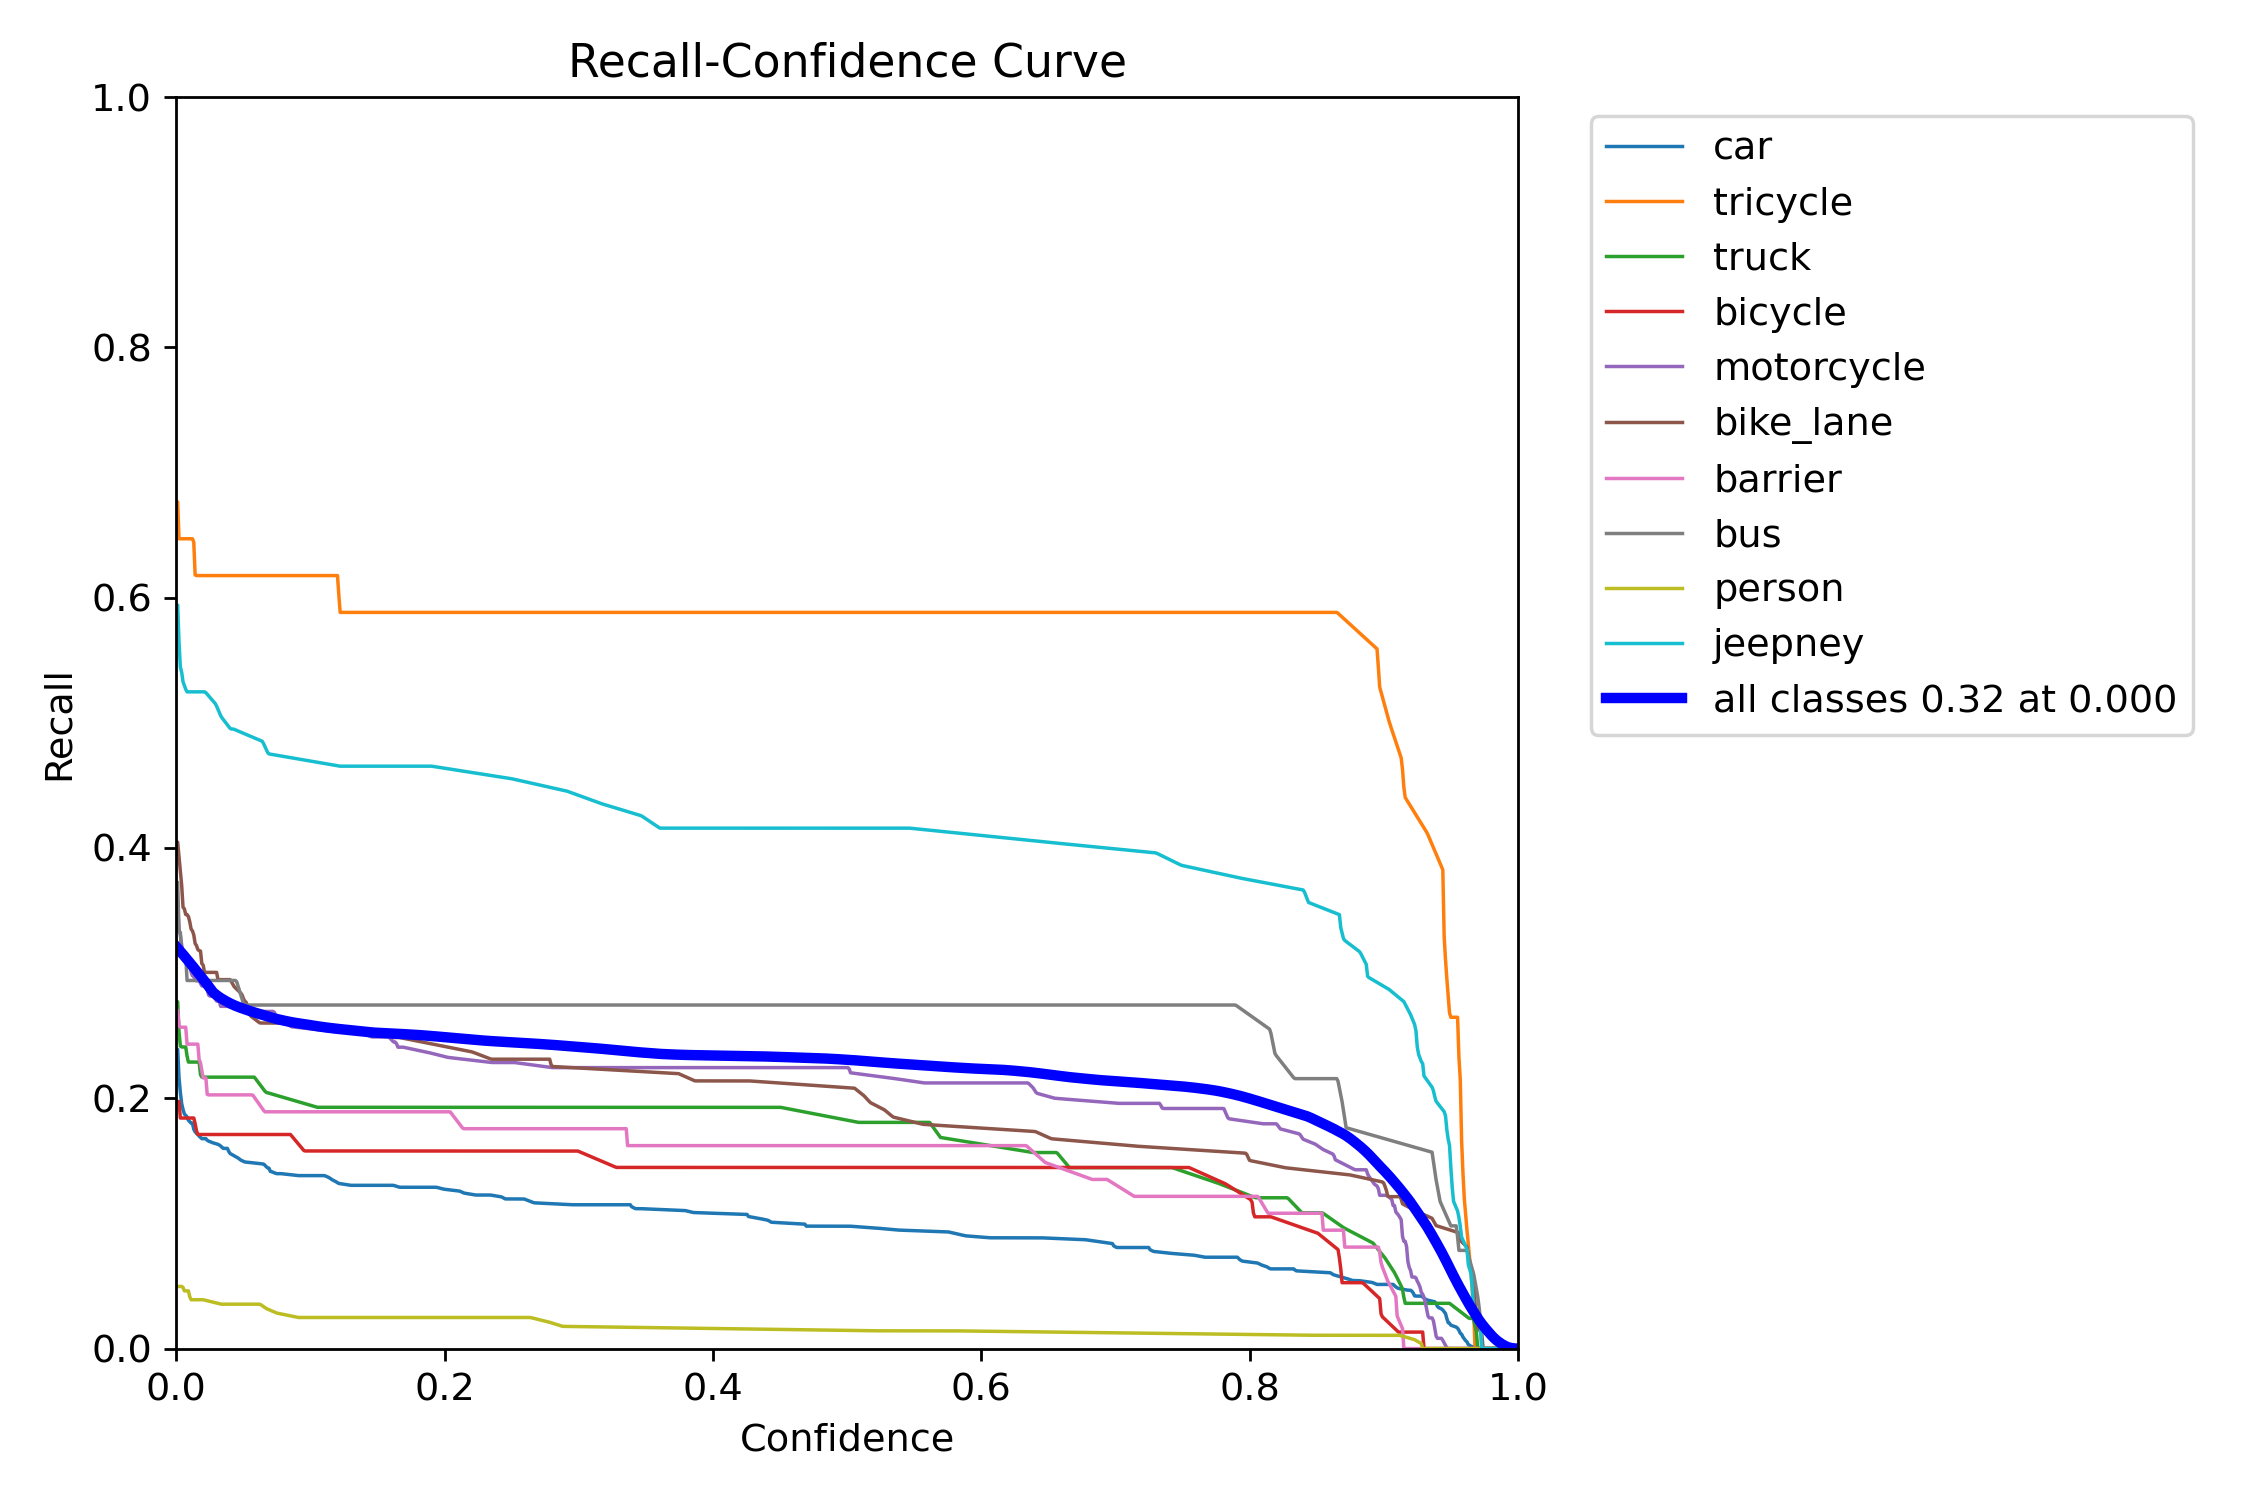
\includegraphics[width=0.75\linewidth]{figures/chapt7/section7.1/MaskR_curve.png}
    \caption{Recall-Confidence Curve for Mask Predictions}
    \label{fig:recall-curve-mask}
\end{figure}

This pattern can be explained by the nature of instance segmentation and the learning dynamics of the model. Mask prediction is a more fine-grained and complex task than bounding-box detection, as it requires accurate pixel-level delineation of object boundaries. This complexity makes segmentation more sensitive to factors such as object size, occlusion, and annotation quality. Classes like \texttt{tricycle} and \texttt{jeepney} have benefited from more consistent shape profiles, distinct features, and better representation in the training data, enabling the model to generate confident and accurate masks for them (as seen in Figure~\ref{fig:recall-mask-imgs1}). Additionally, these objects tend to be larger and less frequently occluded, which simplifies the segmentation task and leads to higher recall.

\begin{figure}[H]
    \centering
    % Row 1
    \begin{subfigure}[b]{0.45\textwidth}
        \centering
        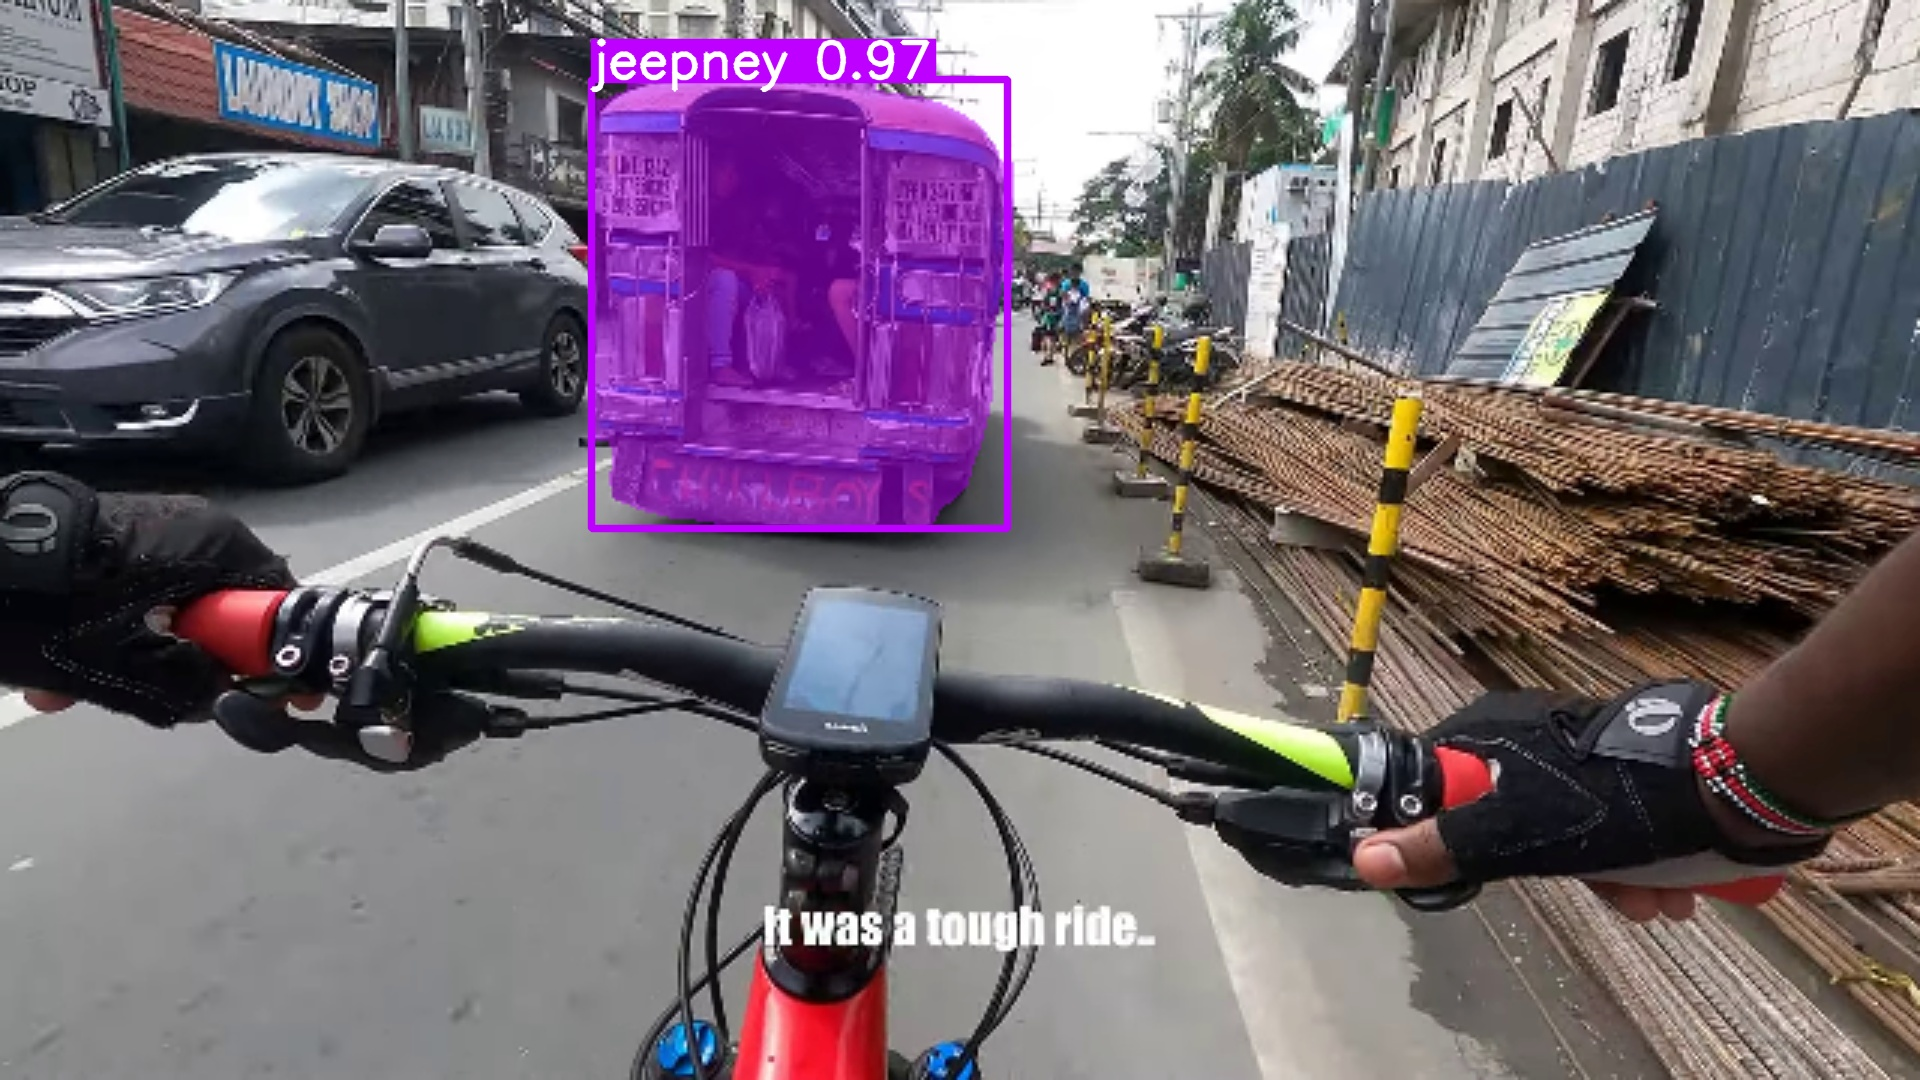
\includegraphics[width=\linewidth]{figures/chapt7/section7.1/inferred_frame_0026.jpg}
        \caption{Good mask segmentation of a \texttt{jeepney} instance}
    \end{subfigure}
    \hfill
    \begin{subfigure}[b]{0.45\textwidth}
        \centering
        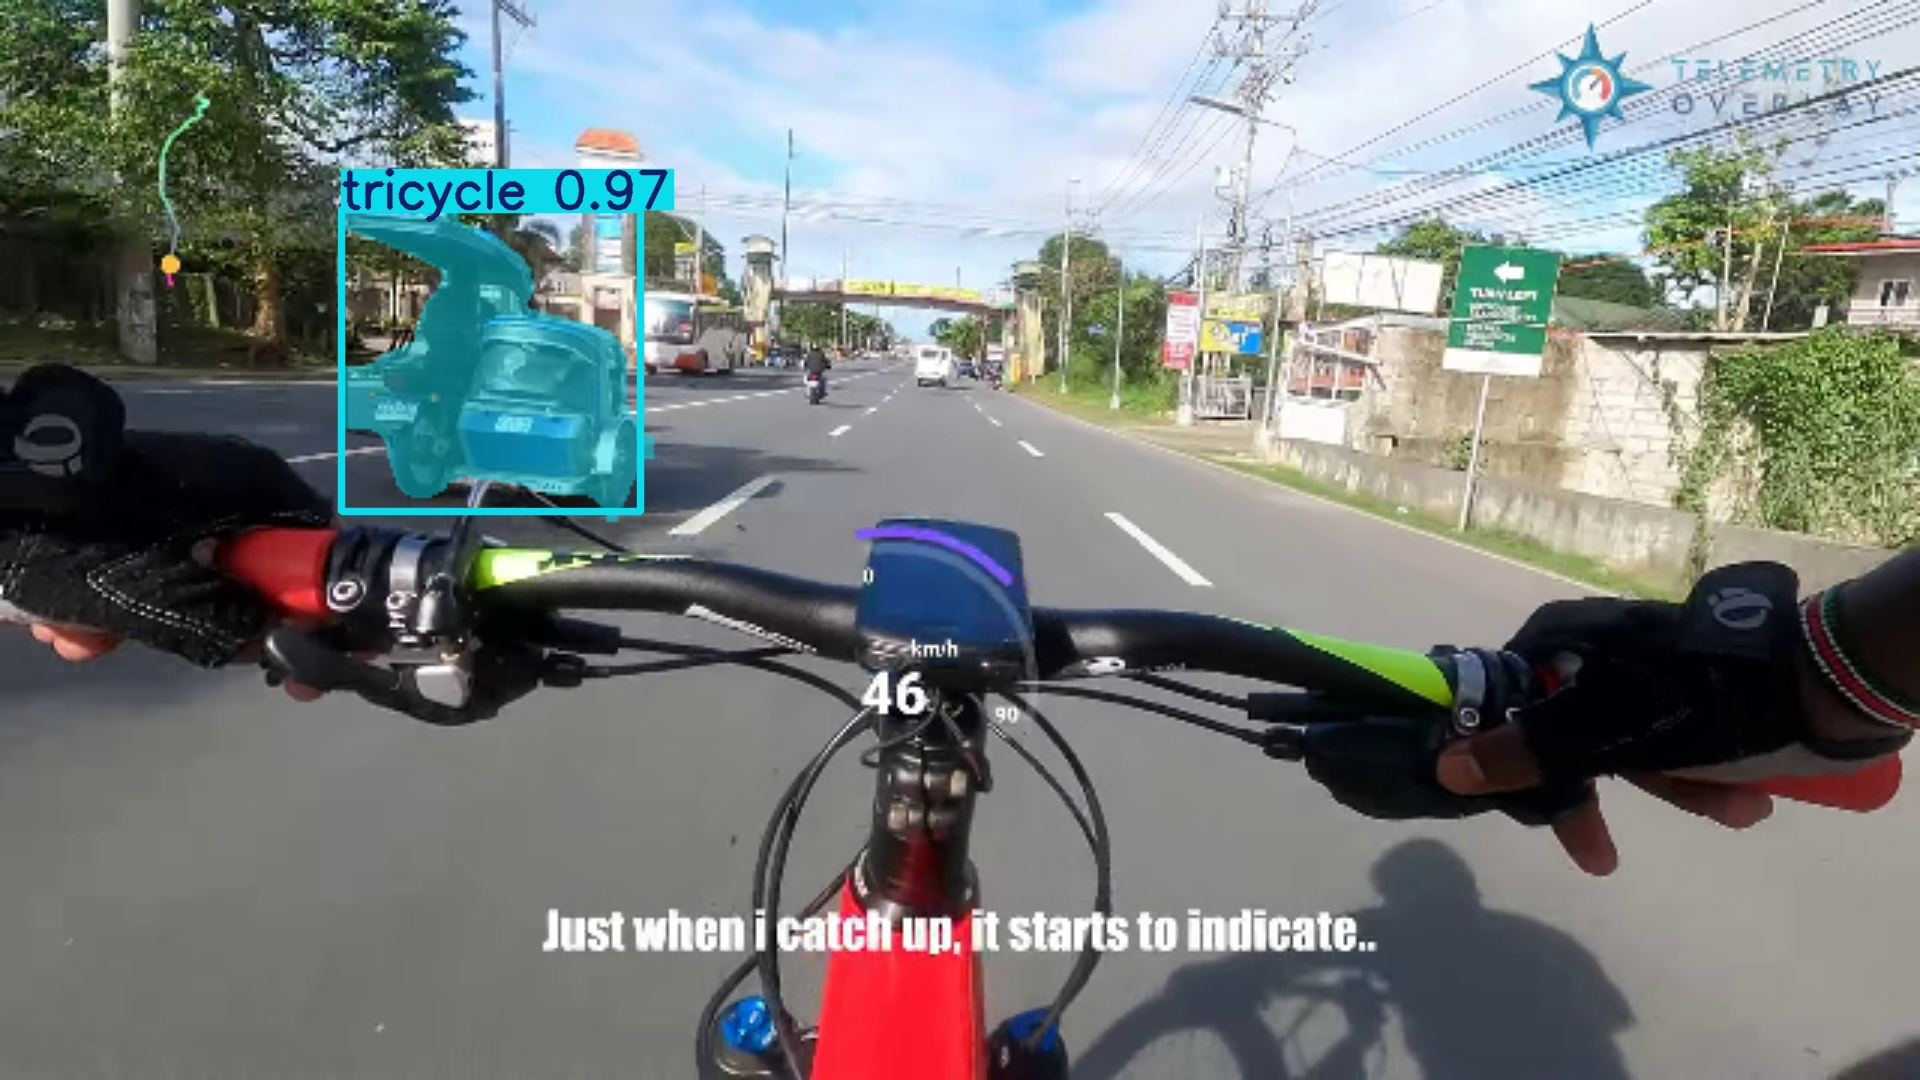
\includegraphics[width=\linewidth]{figures/chapt7/section7.1/inferred_frame_0013.jpg}
        \caption{Good mask segmentation of a \texttt{tricycle} instance}
    \end{subfigure}

    \caption{Sample inferred images with good mask segmentation}
    \label{fig:recall-mask-imgs1}
\end{figure}

On the other hand, classes such as \texttt{person}, \texttt{bicycle}, and \texttt{truck} are often characterized by high intra-class variability, partial occlusions, and background clutter, making it harder for the model to segment them reliably (as seen in Figure~\ref{fig:recall-mask-imgs2}). Some of these classes may have also suffered from underrepresentation in the dataset or annotation inconsistencies, which hindered the model's ability to generalize. The model's design, especially if influenced by detection-first pipelines (e.g., YOLOv11 using box-based region proposals before mask generation), can further bias predictions toward more clearly detectable classes, suppressing recall for more ambiguous ones.

\begin{figure}[H]
    \centering
    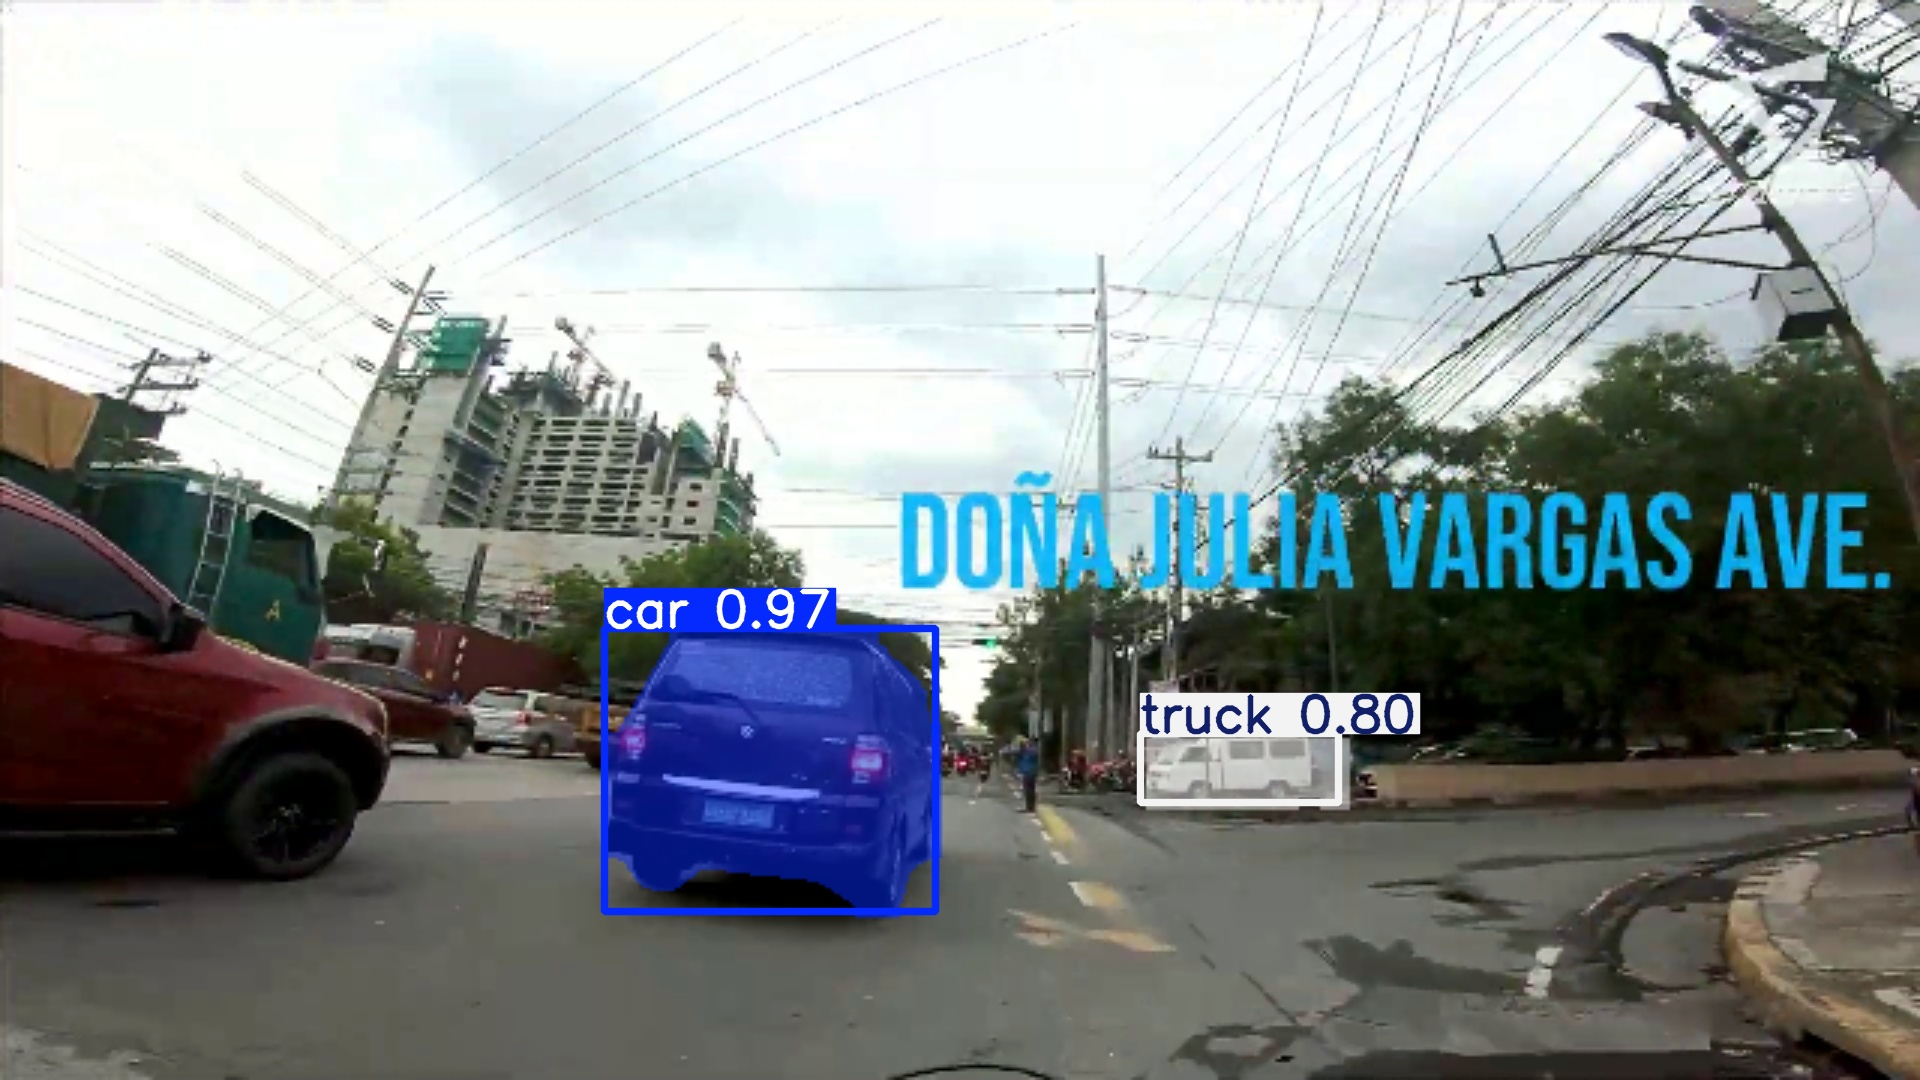
\includegraphics[width=0.45\linewidth]{figures/chapt7/section7.1/inferred_frame_0037.jpg}
    \caption{Bad mask segmentation of a \texttt{truck} instance}
    \label{fig:recall-mask-imgs2}
\end{figure}

Furthermore, the steep decline in recall with increasing confidence reflects a conservative confidence calibration—only a small fraction of mask predictions are assigned high confidence, and many potentially correct predictions are filtered out early. Although this improves precision, it negatively impacts recall, especially for classes that inherently produce less confident predictions.

\subsection{Precision-Recall}

\subsubsection{Box}
The Precision-Recall (PR) Curve (Box), seen in Figure~\ref{fig:prec-recall-box}, reveals moderate detection performance, characterized by a rapid drop in precision as recall increases. This indicates that while the model achieves high precision at lower recall levels (i.e., it makes fewer false positives when detecting only the most confident predictions), its precision sharply declines as it attempts to detect more objects, suggesting an increasing number of false positives. The curve's steep slope and lack of a sustained high-precision region reflect challenges in maintaining accurate bounding box predictions across a broader range of object instances. This pattern typically signals issues with class confusion, poor localization, or imbalanced training data and suggests that while the model is reliable for confident detections, its overall recall and generalization ability may be limited.

\begin{figure}[H]
    \centering
    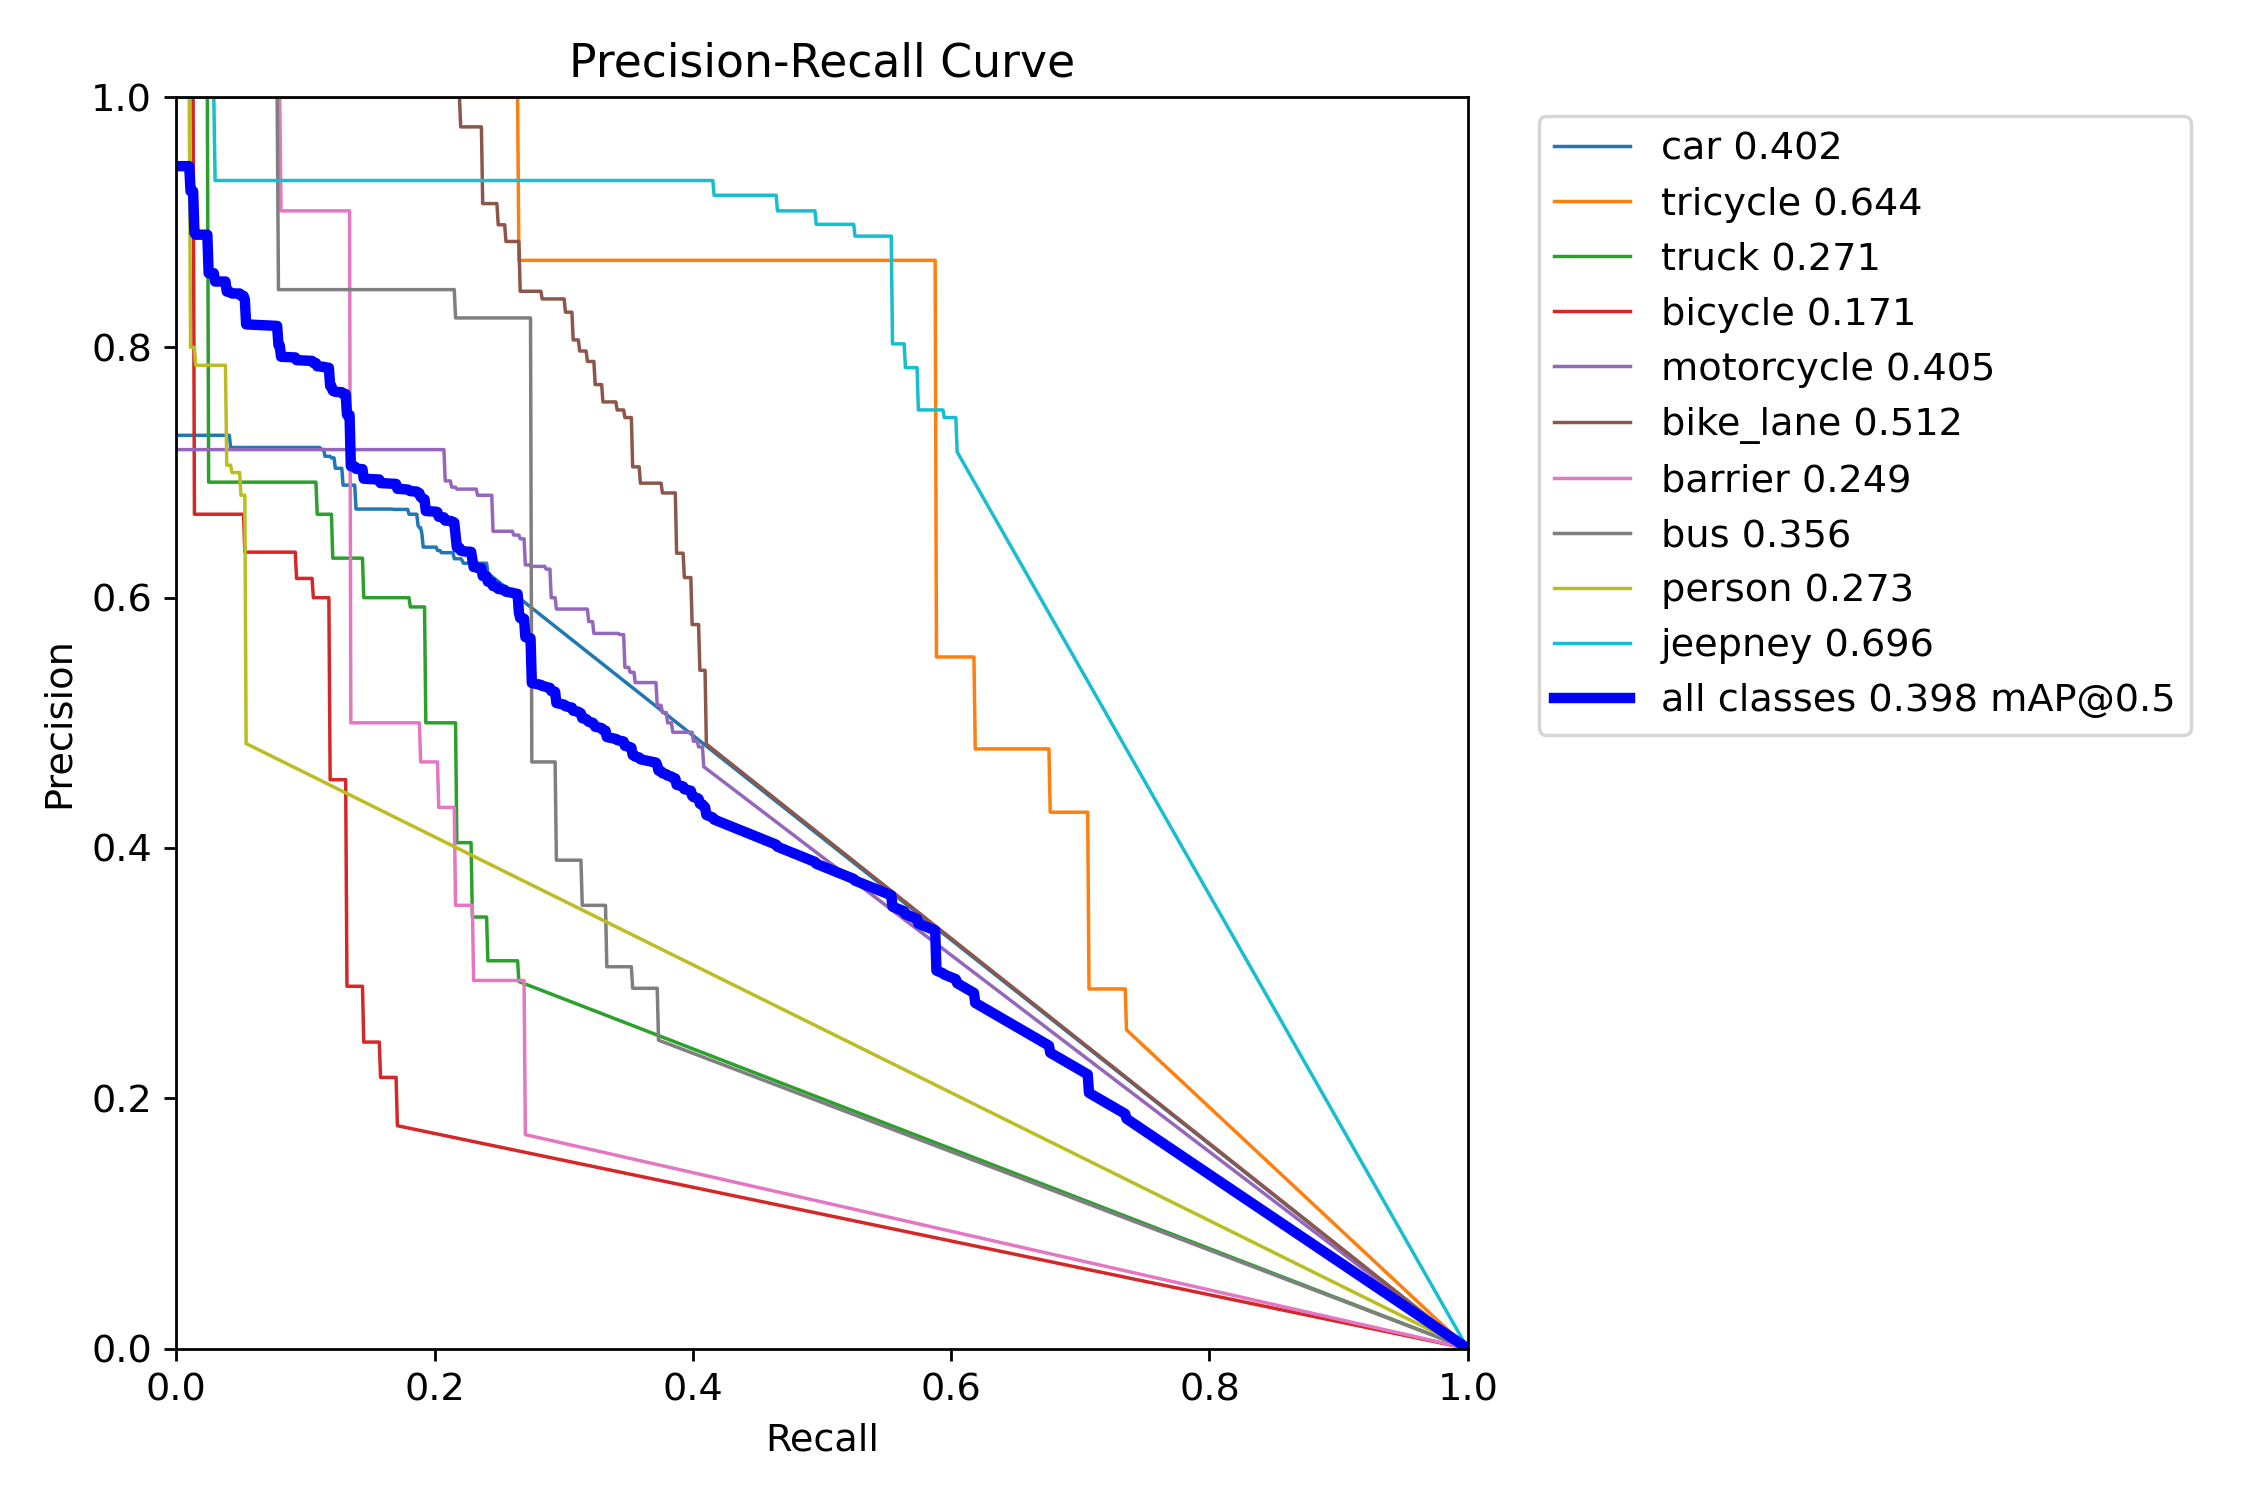
\includegraphics[width=0.75\linewidth]{figures/chapt7/section7.1/BoxPR_curve.png}
    \caption{Precision-Recall Curve for Box Predictions}
    \label{fig:prec-recall-box}
\end{figure}

This behavior can be attributed to several key factors tied to the model architecture, dataset quality, and training dynamics. First, YOLO-based models like YOLOv11 are optimized for speed and real-time performance, which can come at the cost of precise localization, especially for smaller or overlapping objects. As the model is pushed to recall more objects—by lowering the confidence threshold—it includes more uncertain predictions, many of which may be incorrect or poorly localized, thereby reducing precision. This trade-off is typical in one-stage detectors where the dense prediction grid can lead to duplicate or closely placed predictions, especially when non-maximum suppression (NMS) isn't aggressive enough.

Additionally, the lack of a plateau in the precision-recall curve suggests that the model struggles to maintain confident, accurate detections across all object types. This is due to class imbalance, where underrepresented or visually ambiguous classes are not well learned, resulting in more frequent misclassifications as recall increases. Similarly, poor localization quality—as seen in higher box loss values—can produce bounding boxes that overlap poorly with ground truth objects, which harms both precision and recall, particularly at higher IoU thresholds.

Lastly, the steep decline reflects a possible overconfidence calibration issue. The model might assign high confidence to a narrow set of easily identifiable objects (e.g., large or visually distinct ones), but its confidence in other predictions does not correlate well with correctness, leading to an influx of false positives when less confident predictions are included.

\subsubsection{Mask}
The Precision-Recall (PR) Curve (Figure~\ref{fig:prec-recall-mask}) for mask predictions presents the trade-off between precision and recall for various object classes. Each curve represents a class's performance at different recall thresholds. For instance, the \texttt{jeepney} class shows the highest precision and recall, peaking at a recall of 0.7 with a precision of around 0.7, suggesting a strong ability to identify jeepneys without a significant drop in precision. On the other hand, the \texttt{barrier} and \texttt{bicycle} classes exhibit lower performance, with precision dropping rapidly as recall increases, indicating a higher false-positive rate. The thick blue curve, representing the average performance across all classes, has a mean Average Precision (mAP) of 0.387 at a recall threshold of 0.5, signifying moderate overall performance. The precision drops steadily across most classes, and the model struggles to maintain high precision when attempting to capture a higher number of true positives (increasing recall), especially for underrepresented classes like \texttt{barrier} and \texttt{bus}.

\begin{figure}[H]
    \centering
    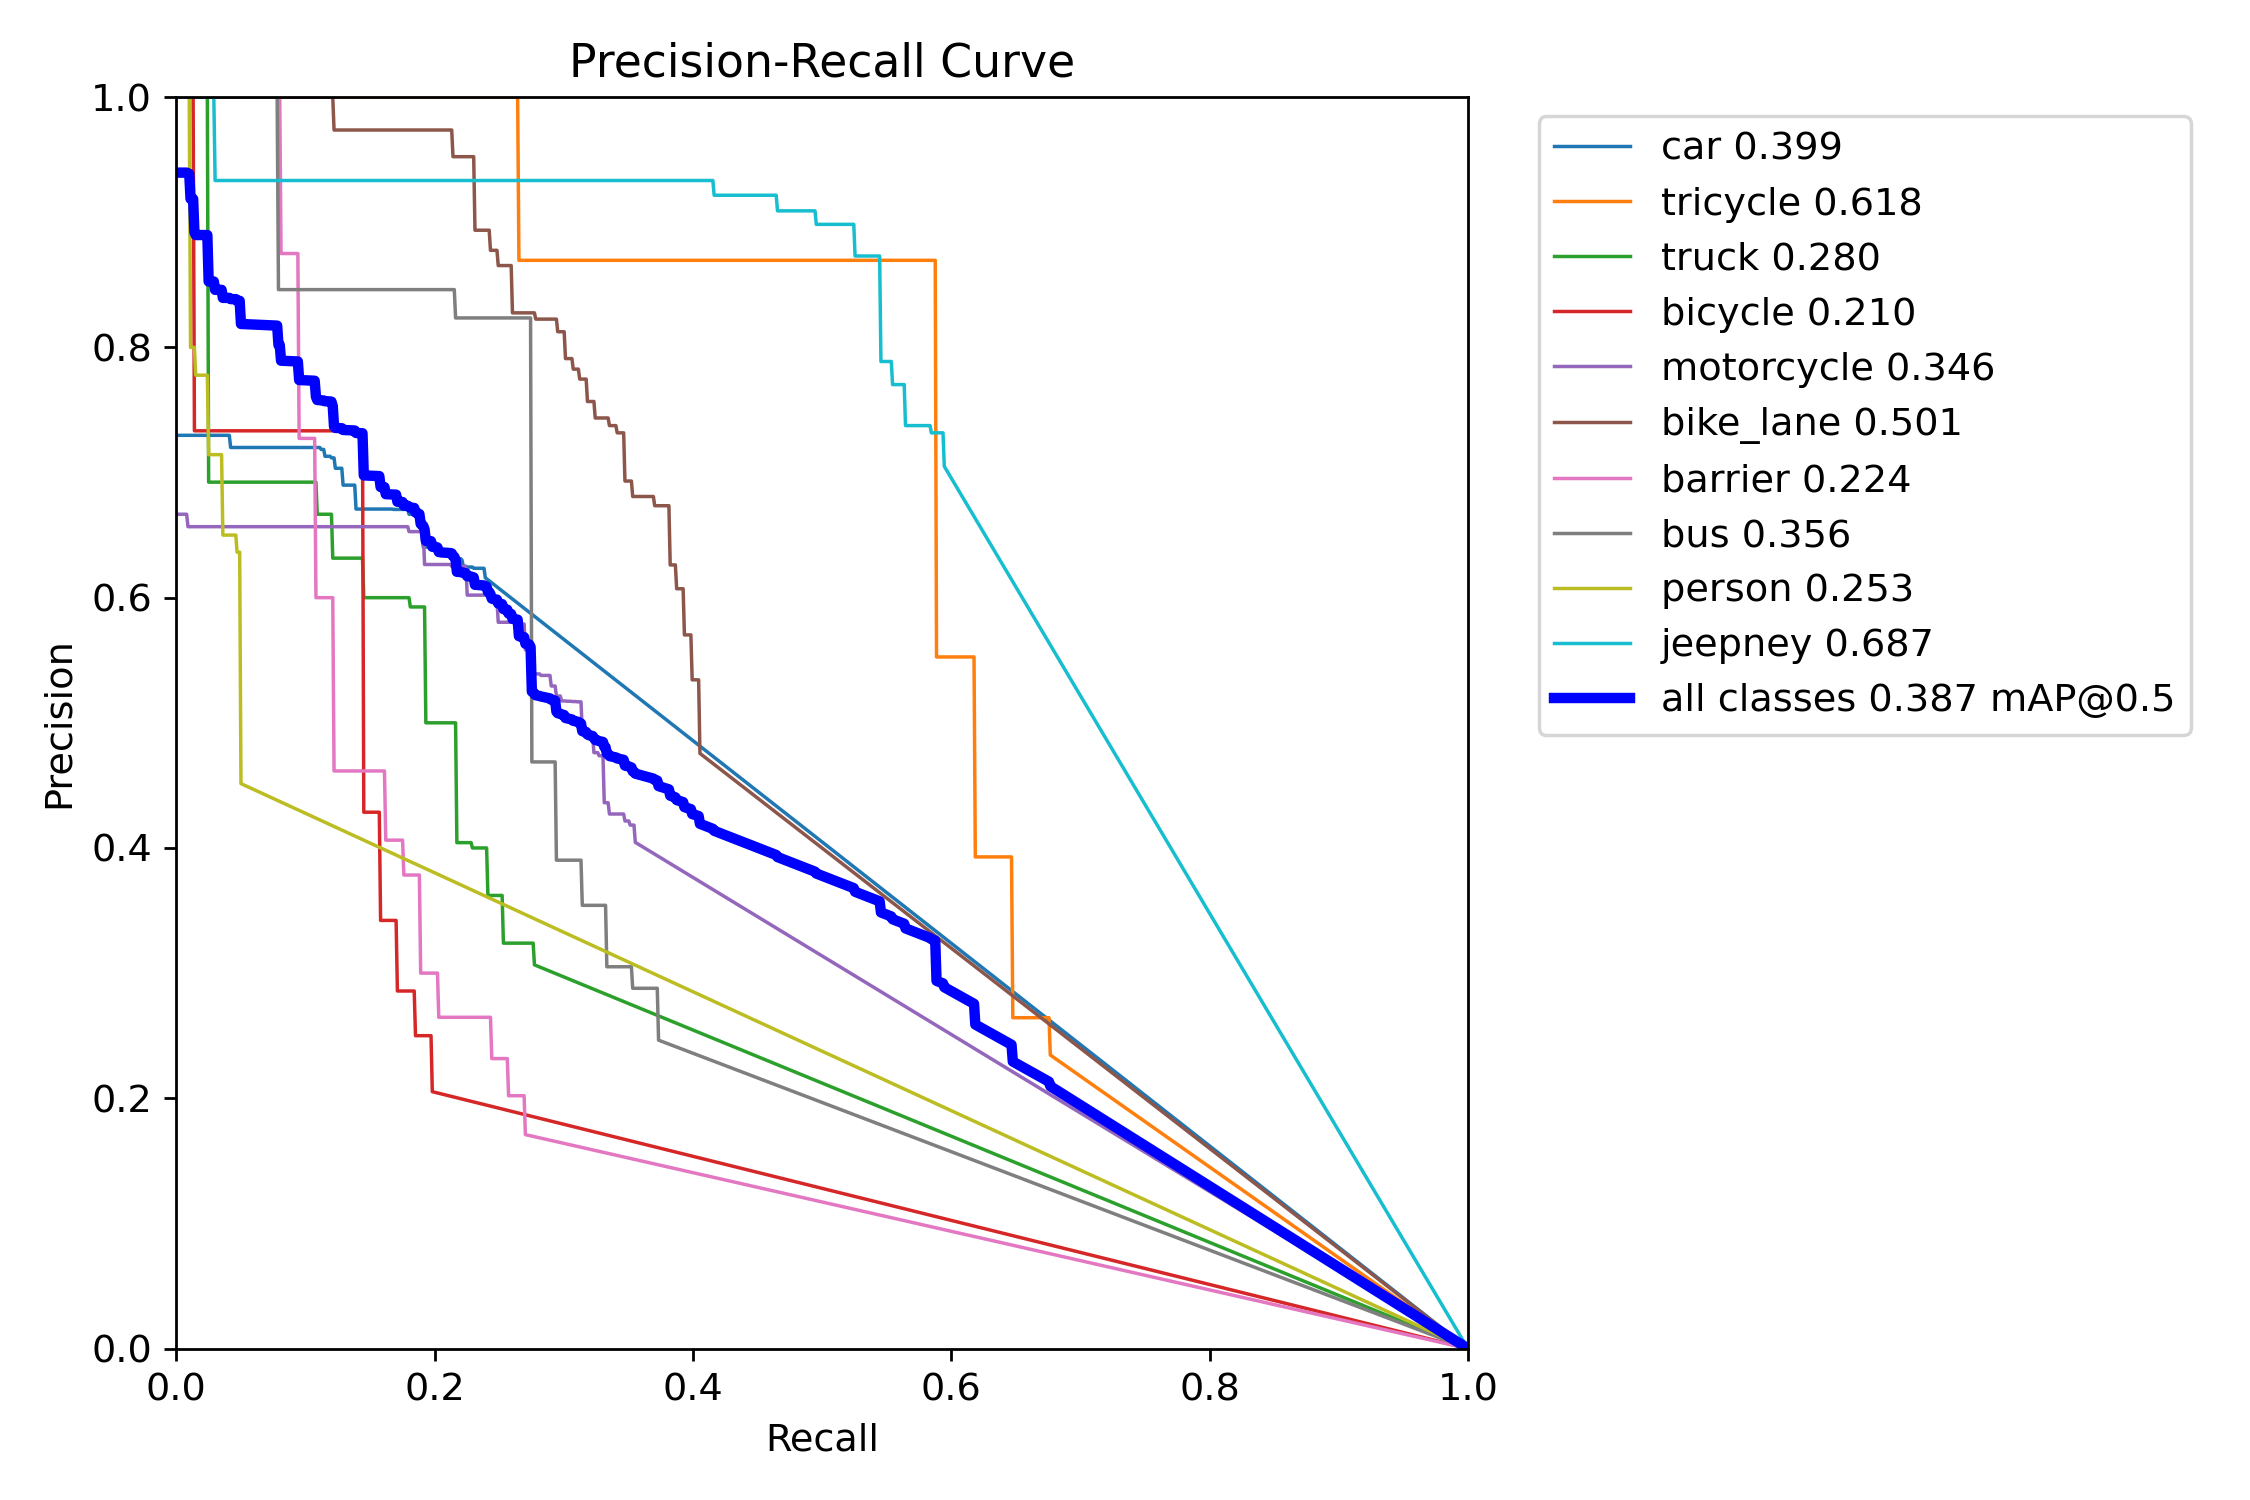
\includegraphics[width=0.75\linewidth]{figures/chapt7/section7.1/MaskPR_curve.png}
    \caption{Precision-Recall Curve for Mask Predictions}
    \label{fig:prec-recall-mask}
\end{figure}

This performance pattern can be explained by the inherent challenges of instance segmentation and class-specific variability in visual representation. The \texttt{jeepney} class benefits from several favorable factors: it was well-represented in the training data, exhibited large and distinct shapes, and possessed unique visual features that made it easier for the model to segment accurately. As a result, the model can detect jeepneys with a relatively balanced trade-off between precision and recall.

In contrast, classes like \texttt{barrier}, \texttt{bicycle}, and \texttt{bus} often present segmentation difficulties due to their small size, visual similarity to background elements, or partial occlusions in real-world scenes. These issues led to both false positives (e.g., misidentifying parts of the environment as a barrier) and false negatives (failing to detect partially visible or overlapping objects), especially when the model is forced to make more predictions at lower confidence thresholds. These classes may have also been underrepresented in the training data, which limits the model's ability to generalize well to new instances.

Furthermore, the steady decline in precision across most classes as recall increases is a typical pattern in models that are confidence-calibrated conservatively—they assign high confidence only to very certain predictions. As the recall threshold increases (i.e., when more predictions are included), many of the additional detections come from less confident, and often less accurate, predictions. This introduces more false positives and reduces precision. The model's architectural bias—optimized for fast, detection-first segmentation—may also led to less accurate masks when object boundaries are complex or ambiguous.

\subsection{F1 Score}

\subsubsection{Box}
The F1-Confidence Curve for box predictions, seen in Figure~\ref{fig:f1-box}, demonstrates how the F1 score (the harmonic mean of precision and recall) varies with confidence thresholds across various object classes. The blue curve represents the overall performance of all classes, stabilizing around an F1 score of 0.35 at a confidence of 0.028, which suggests a moderate overall balance between precision and recall. Classes like \texttt{jeepney} and \texttt{tricycle} exhibit higher F1 scores, peaking around 0.6–0.7, reflecting relatively better performance in terms of both precision and recall at higher confidence levels. However, for classes like \texttt{barrier} and \texttt{person}, the F1 scores remain low, indicating that the model struggles to achieve a good balance between precision and recall for these classes, even as confidence increases. The rapid decrease in F1 scores for many classes after the confidence exceeds certain thresholds suggests that the model's precision improves with higher confidence, but it also misses a significant number of true positives, thus lowering recall and, ultimately, the F1 score. This pattern highlights the trade-off between precision and recall, with the model favoring precision at the cost of recall in higher-confidence predictions.

\begin{figure}[H]
    \centering
    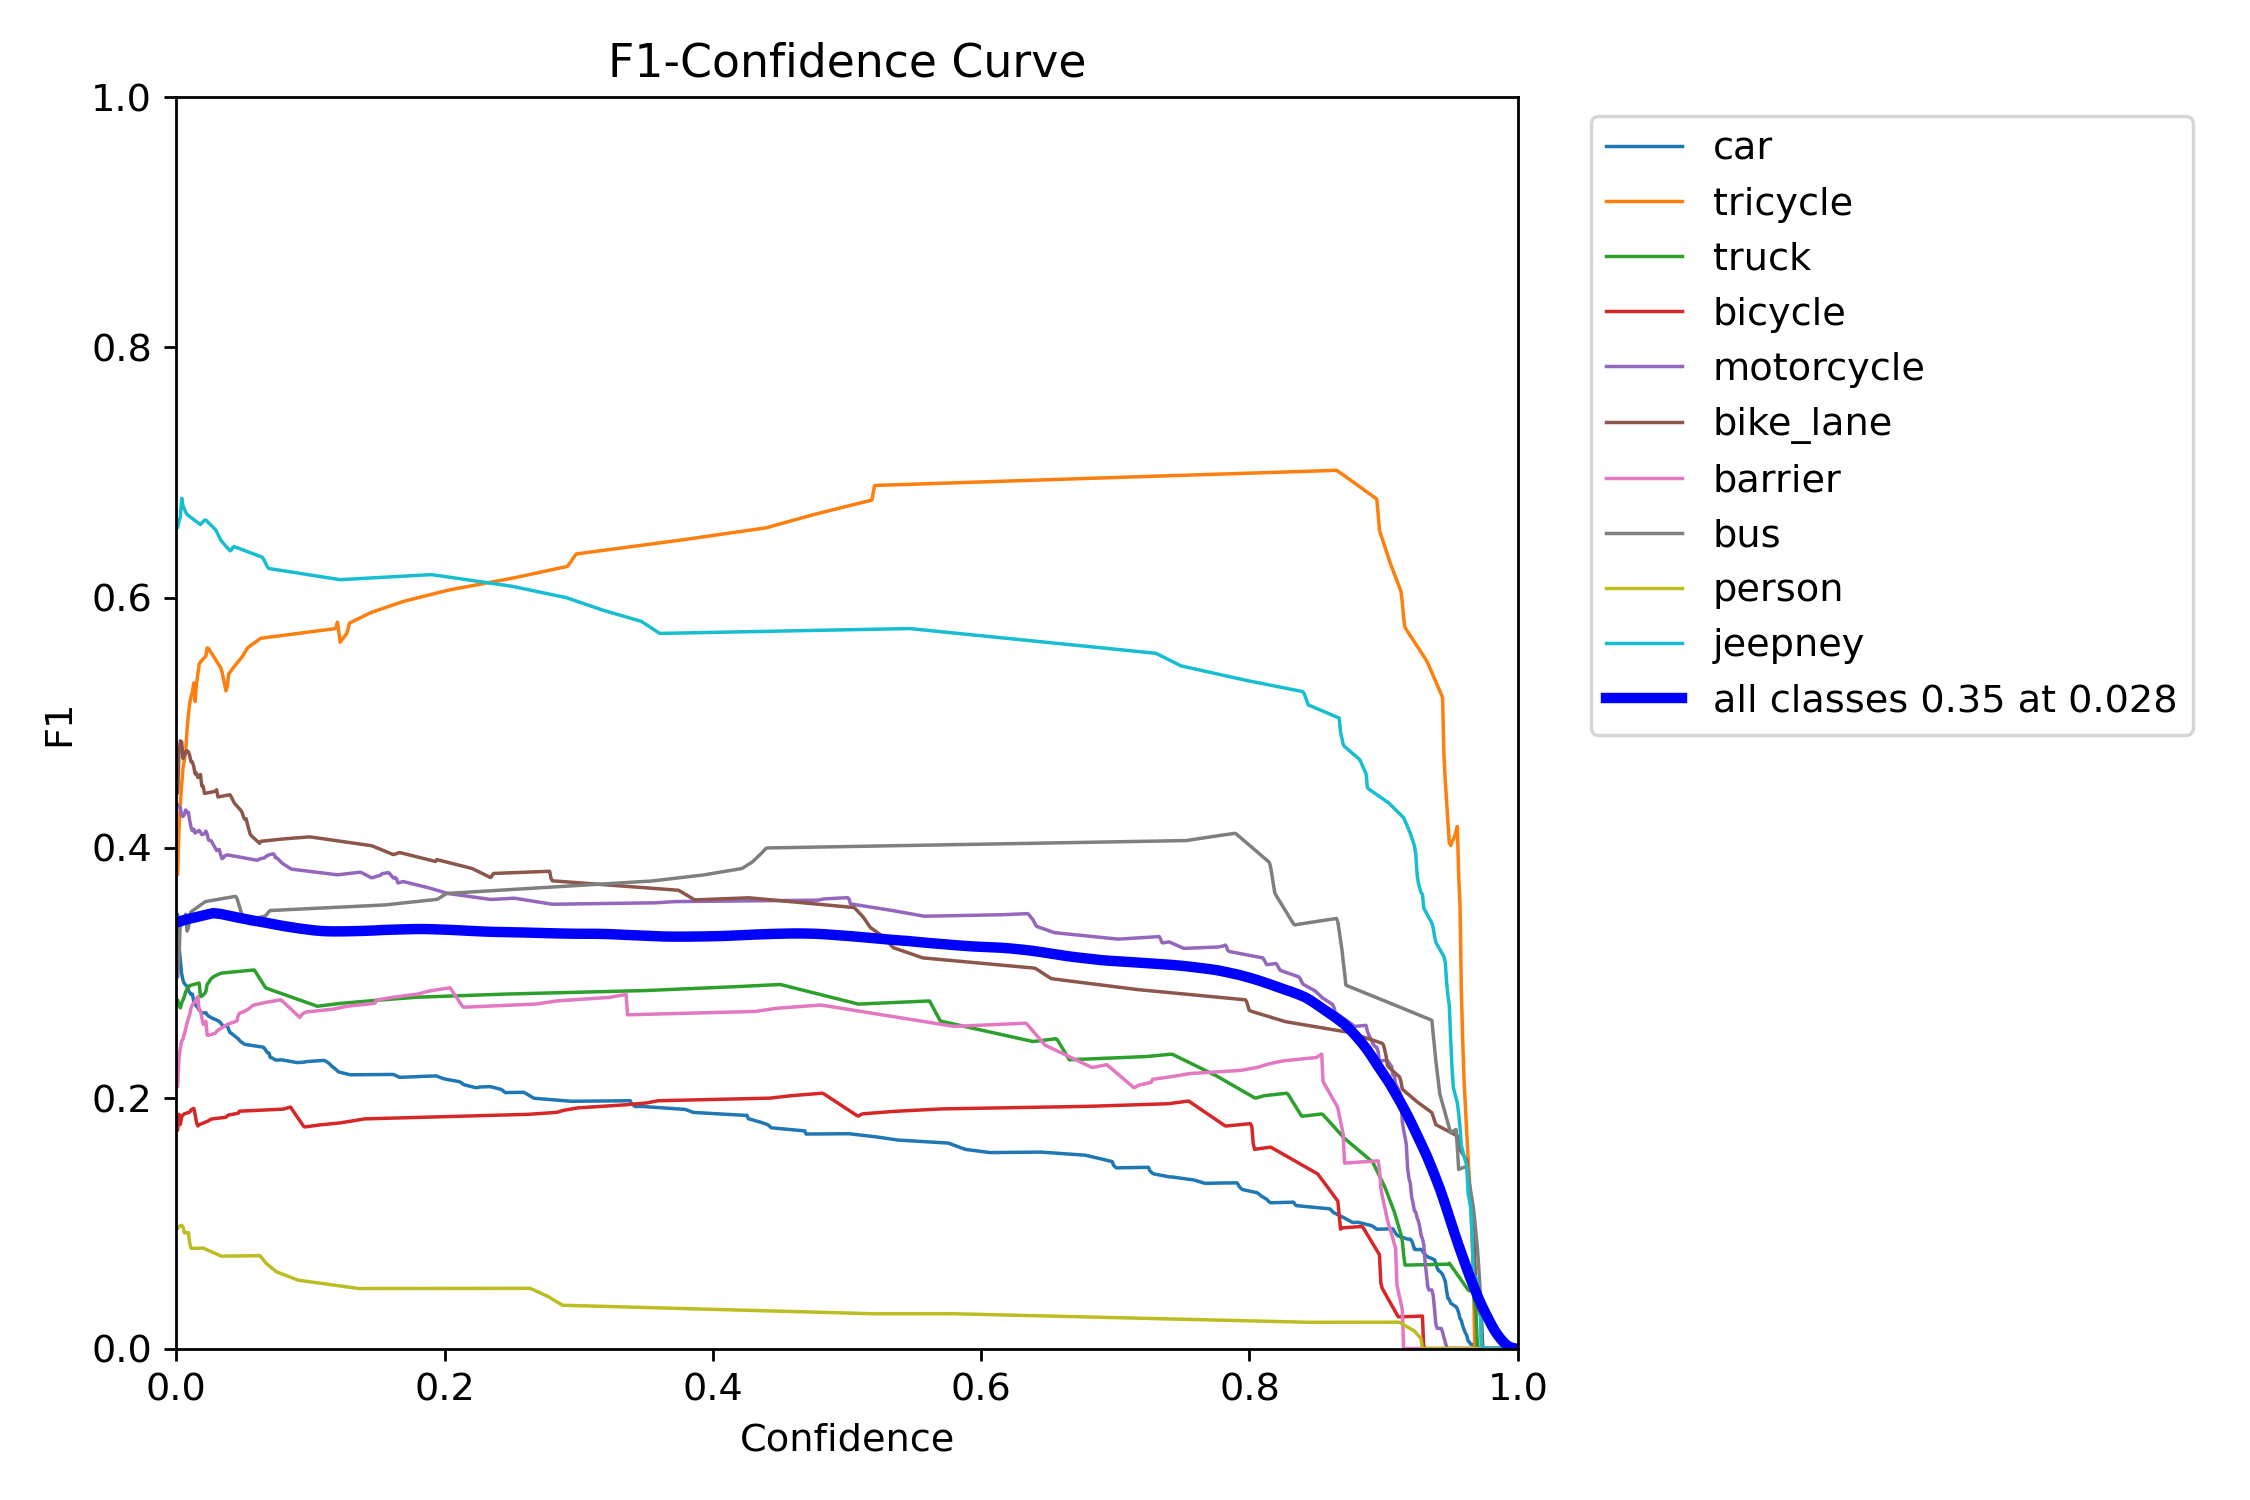
\includegraphics[width=0.75\linewidth]{figures/chapt7/section7.1/BoxF1_curve.png}
    \caption{F1-Confidence Curve of the Fine-Tuned YOLOv11l Model}
    \label{fig:f1-box}
\end{figure}

This behavior can be attributed to several interrelated factors affecting the model's detection performance. First, the F1 score inherently penalizes imbalances between precision and recall—so any shift toward higher precision at the expense of recall, which occurs at high confidence thresholds, results in a lower F1 score. The model's tendency to assign high confidence only to highly certain predictions reflects a conservative prediction strategy. While this improves the precision for classes with distinct visual features and clear object boundaries (like \texttt{jeepney} and \texttt{tricycle}), it also means many valid but less certain detections are filtered out, reducing recall.

For classes like \texttt{barrier} and \texttt{person}, the lower F1 scores across all confidence thresholds suggest persistent detection challenges. These could stem from several causes: smaller object sizes, occlusions, visual ambiguity, or the class imbalance in the training data. Since these classes may have been underrepresented or poorly annotated, the model may have failed to learn robust and generalizable features, which led to both low precision (more false positives) and low recall (more false negatives).

The sharp decline in F1 scores beyond certain confidence levels also reflects how the model's calibration does not generalize well across all object classes. For easier-to-detect classes, high confidence scores align with accurate predictions. However, for harder classes, the model lacks sufficient certainty and tends to underpredict, causing a drop in recall when the threshold increases. This imbalance between class-level performance further drives down the macro-average F1 score at higher confidence levels.

\subsubsection{Mask}
The F1-Confidence Curve for mask predictions, seen in Figure~\ref{fig:f1-mask}, also illustrates the balance between precision and recall (F1 score) across various object classes as confidence thresholds increase. The blue curve representing the average performance across all classes stabilizes at an F1 score of 0.34 around a confidence threshold of 0.029, indicating moderate overall performance. Some classes, like \texttt{jeepney} and \texttt{tricycle}, maintain relatively higher F1 scores of around 0.6, showing that the model performs better for these classes, maintaining a reasonable balance between precision and recall. However, other classes such as \texttt{barrier} and \texttt{person} show much lower F1 scores, indicating poor performance in terms of both precision and recall. The rapid decrease in F1 scores for most classes as the confidence increases suggests that while precision improves, recall drops significantly, highlighting that the model tends to be more conservative, favoring higher precision at the cost of missing more true positives, especially at higher confidence levels.

\begin{figure}[H]
    \centering
    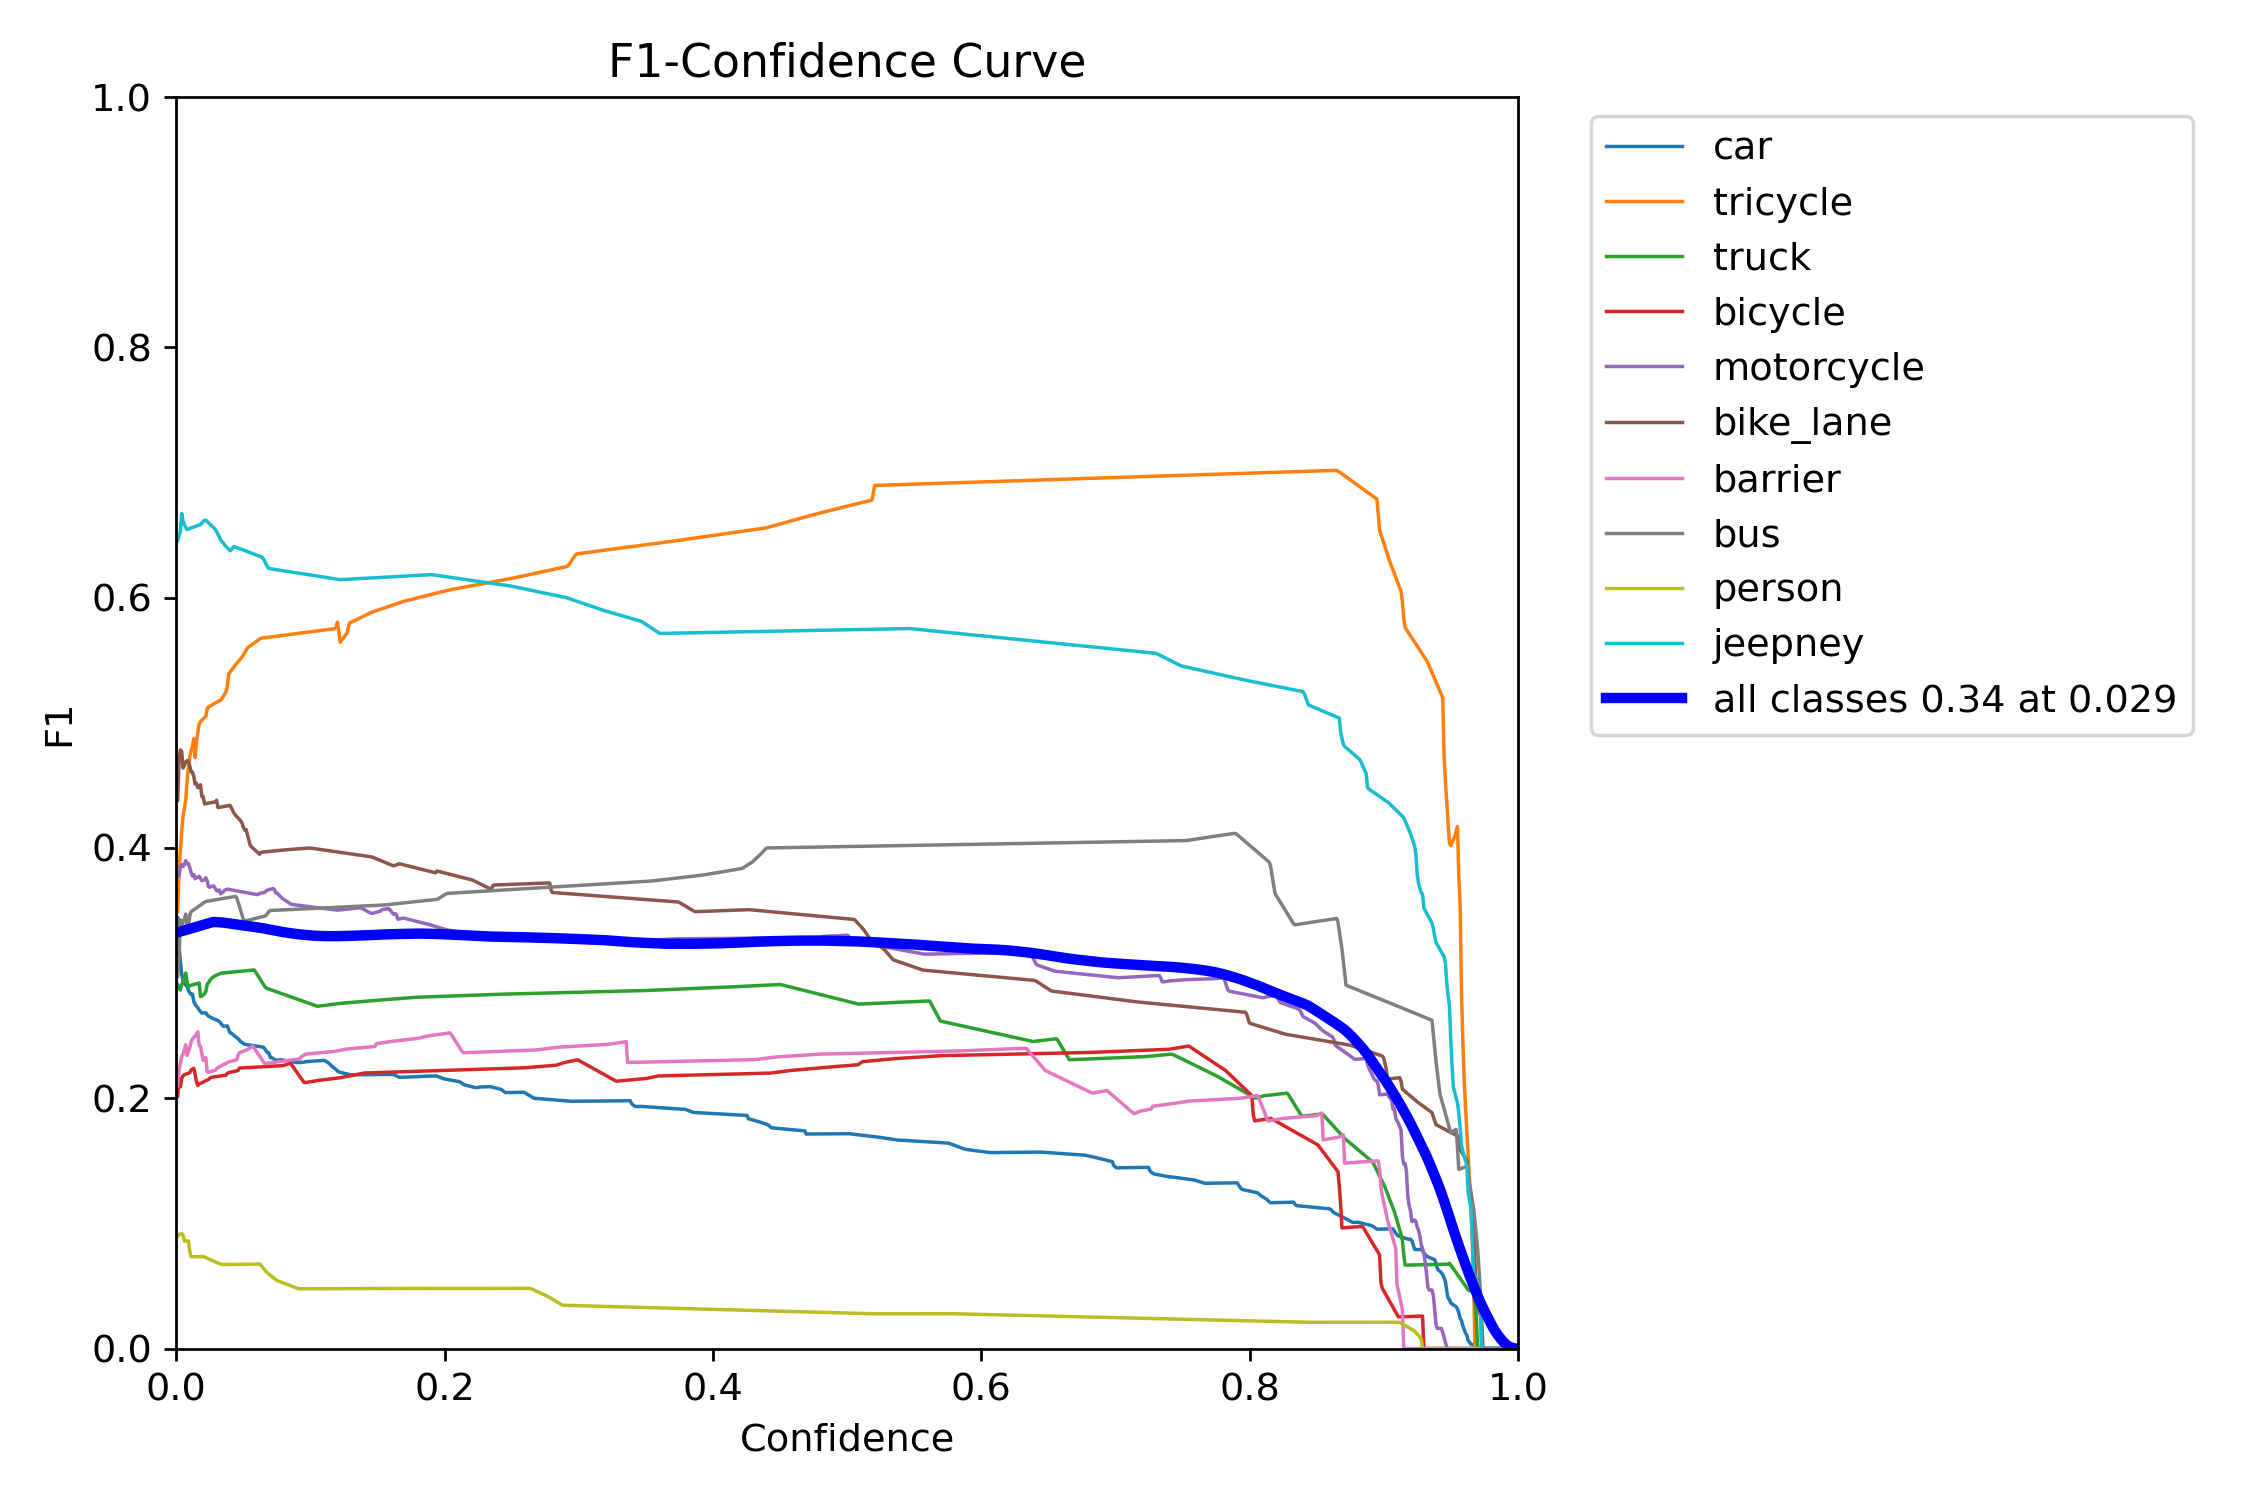
\includegraphics[width=0.75\linewidth]{figures/chapt7/section7.1/MaskF1_curve.png}
    \caption{F1-Confidence Curve of the Fine-Tuned YOLOv11l Model}
    \label{fig:f1-mask}
\end{figure}

This behavior is largely influenced by the complexity of instance segmentation tasks, where the model must not only localize objects but also generate accurate pixel-level masks. For well-defined and visually distinct classes like \texttt{jeepney} and \texttt{tricycle}, the model can confidently generate accurate masks with fewer overlaps or ambiguities, resulting in better precision and recall—and thus, higher F1 scores. These classes have more consistent visual patterns, sufficient training examples, and larger object sizes, which all contribute to more reliable predictions.

In contrast, classes like \texttt{barrier} and \texttt{person} pose significant challenges. Barriers are often small, occluded, or visually similar to the background (e.g., bollards, concrete barriers), making it difficult for the model to segment them accurately. Similarly, persons often appear in crowded or dynamic scenes, leading to overlapping instances and higher mask ambiguity. These conditions contribute to false positives (over-segmentation or misclassification) and false negatives (missed detections), especially at high confidence thresholds where the model filters out uncertain predictions to preserve precision—resulting in a sharp drop in recall.

Additionally, the drop in F1 scores at higher confidence levels indicates that while the model becomes stricter in what it considers a valid detection (thus improving precision), it also sacrifices recall by ignoring many true positives that don't meet the high confidence bar.

Lastly, the difficulty of generating precise instance masks (as opposed to just bounding boxes) adds another layer of complexity. Even small inaccuracies in mask prediction resulted in lower intersection-over-union (IoU) scores, leading to poor evaluation metrics—even if the object is detected correctly in general terms. This further explains why F1 scores degrade more rapidly for complex or fine-grained object classes in the segmentation task compared to detection.

\subsection{Inference on Crowdsourced Data}

After training, the fine-tuned YOLOv11-Large model was deployed via a dedicated inference API integrated into the WeCyclePH mobile platform. Cyclists recorded POV videos during their rides, which were subsequently uploaded and split into frames. Each frame was passed through the inference pipeline, and detected object classes were counted and aggregated per trip to support downstream analysis of cycling infrastructure conditions.

\subsection{Implications and Limitations}
The deployed YOLOv11-Large instance segmentation model, while not without its limitations, plays a valuable role in advancing the objectives of the WeCyclePH project. By automating the extraction of key infrastructure features from cyclist-submitted videos, the model facilitates scalable, semi-structured analysis of Philippines' urban cycling environments. When integrated with trip-level data aggregation, the segmentation outputs can support several critical applications: identifying road segments prone to obstacles, generating quantitative assessments of bike lane presence and road surface conditions, and cross-validating user-submitted annotations. However, the model's performance reveals notable areas for improvement. Low recall—particularly for underrepresented or small object classes—highlights the need for dataset augmentation, class balancing, and more robust training strategies. Additionally, the reliance on cloud-based inference introduces latency, hindering real-time feedback capabilities for users. To address these issues, future work should consider multi-scale training techniques and attention mechanisms to enhance detection accuracy, explore on-device inference to reduce latency, and implement semi-supervised or active learning approaches that leverage user-submitted failure cases for iterative model refinement. In summary, the model shows promising accuracy for detecting prominent road features and serves as a solid foundation for WeCyclePH's platform deployment, yet further development is essential to improve detection breadth, reliability, and responsiveness—particularly for infrastructure elements crucial to cyclist safety.

\section{Mobile Application Evaluation}

This section presents the evaluation of the WeCyclePH mobile application based on findings gathered during the Public Beta Feedback Gathering phase. Through a mixed-methods approach that combined quantitative metrics from the User Experience Questionnaire (UEQ) and qualitative insights from semi-structured interviews, the evaluation aimed to assess the platform's usability, emotional engagement, and contribution experience from the perspective of real-world cyclists. The public beta period provided a critical opportunity to observe how users interacted with core features such as ride logging, annotations, and media uploads under authentic cycling conditions.

% \subsection{Public Beta Feedback Gathering}
% \label{sec:PublicBetaFeedBack}

\subsection{User Experience Questionnaire (UEQ) Results}


\begin{figure}[H]
    \centering
    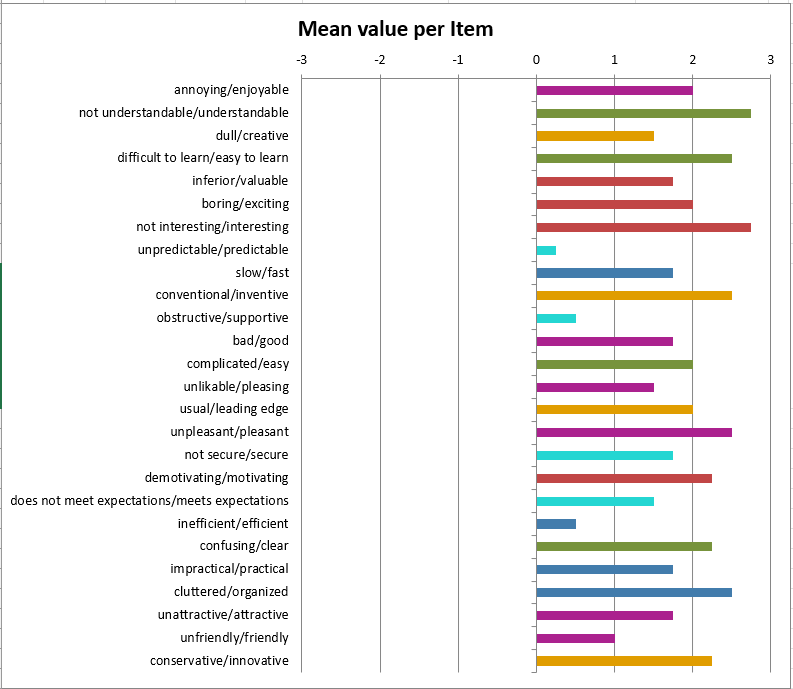
\includegraphics[width=1\linewidth]{figures/chapt7/section7.2/UEQ_Results_ItemCharts.png}
    \caption{Mean scores for each User Experience Questionnaire (UEQ) item, showing participants’ evaluations across usability, satisfaction, and engagement aspects of the WeCyclePH platform.}
    \label{fig:UEQItems}
\end{figure}

As shown in Figure~\ref{fig:UEQItems}, which presents the mean scores per item, the majority of responses clustered within the positive range (above +0.8), indicating a generally favorable user experience. Notably, items such as \textit{understandable} (mean: 2.8), \textit{interesting} (2.8), and \textit{organized} (2.5) received the highest ratings, reflecting strong user perceptions of clarity, engagement, and structural coherence. In contrast, a few items, such as \textit{efficient} (0.5) and \textit{supportive} (0.5), scored comparatively lower, though they still fell within the neutral-to-positive spectrum. The distribution of these item scores suggests that users consistently valued the app's intuitiveness and emotional appeal, while also highlighting minor concerns related to performance speed and reliability. These detailed item-level results surface specific user expectations and potential pain points that may not be evident in aggregated scale-level metrics.


% ** Figure: UEQ Scale Summary with Error Bars
\begin{figure}[H]
    \centering
    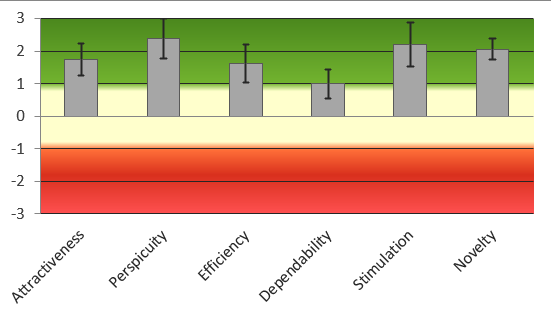
\includegraphics[width=1\linewidth]{figures/chapt7/section7.2/UEQ_Results_ScalesChart.png}
    \caption{Summary of User Experience Questionnaire (UEQ) scale scores with error bars, indicating postive average participant ratings and variability across the six measured user experience dimensions.}
    \label{fig:UEQScales}
\end{figure}

Among the six UEQ scales, Perspicuity (2.38) and Stimulation (2.19) received the highest scores (see Figure \ref{fig:UEQScales}), indicating that users perceived the app as easy to understand, motivating, and exciting. The Novelty scale also performed well at 2.06, showing that the app was regarded as creative and innovative. Meanwhile, Dependability (1.00) and Efficiency (1.63) scored positively but comparatively lower, pointing to minor concerns about predictability, reliability, and performance smoothness, particularly in tasks involving uploads or media-heavy interactions.

% ** Figure : Pragmatic and Hedonic Quality Scores
\begin{figure}[H]
    \centering
    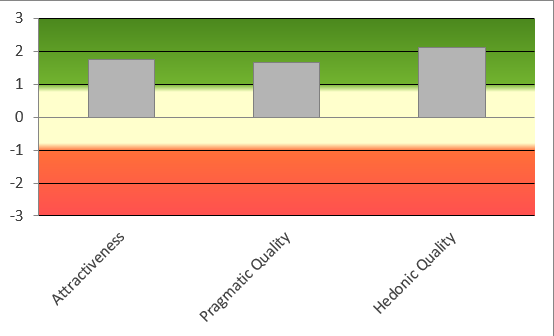
\includegraphics[width=1\linewidth]{figures/chapt7/section7.2/UEQ_Results_PragmaticAndHedonic.png}
    \caption{Pragmatic and Hedonic Quality scores from the User Experience Questionnaire (UEQ), comparing participants’ evaluations of the platform’s practical usability and overall enjoyment.}
    \label{fig:UEQPragmaticHedonic}
\end{figure}

These scale scores are further synthesized in Figure \ref{fig:UEQPragmaticHedonic}, which groups them into Pragmatic Quality (1.67) and Hedonic Quality (2.13). This shows that while the application supports effective task completion, its strength lies in fostering positive emotional engagement and novelty. Taken together, the results affirm that WeCyclePH is well-received for its core functionality, while also offering a stimulating and aesthetically appealing experience. Minor improvements in clarity of feature access and media performance could further enhance the user experience.

\subsection{Thematic Analysis Results}
\label{sec:thematic_analysis_results}
This section presents the thematic analysis of user interviews conducted during the public and closed beta phases of WeCyclePH. The goal of this analysis was to understand not only what users experienced while interacting with the application, but also the deeper motivations, values, and contextual factors that shaped their engagement and contribution behavior.

The resulting themes reflect the perspectives of cyclists with varying levels of experience, each revealing a distinct aspect of how users perceived, valued, and interacted with the WeCyclePH platform. The analysis goes beyond surface-level summaries to highlight what participants prioritized: safety, ease of use, community impact, personal recognition, and autonomy in contribution. These insights inform the broader understanding of user needs and expectations in the context of crowdsourced cycling data platforms.

The following subsections detail four key themes that emerged from the analysis, each supported by verbatim quotes from participants and interpreted in relation to the platform's design and implementation.

\subsubsection{Cyclists Value Safety and Ride Flow Over Manual Contribution}

For many cyclists, maintaining physical safety and an uninterrupted riding rhythm is more important than the opportunity to contribute data during their trips. While users generally found WeCyclePH's annotation feature promising, the act of stopping to report hazards was often perceived as intrusive, risky, or impractical, especially in urban or high-traffic environments. This reveals that real-time contribution must align with the natural flow of riding, or users will simply skip it.

Participants repeatedly cited the difficulty of stopping mid-ride due to safety concerns, environmental conditions, or physical discomfort. These barriers weren't just technical, they were reflections of what users prioritized in their cycling experience: staying safe, keeping momentum, and avoiding distraction.

\begin{quote}
``What's only hard for me is that I need to stop always to report something… I need to worry about hazards like cars in the back or if the area is safe to stop by.'' – \textbf{P2}
\end{quote}

\begin{quote}
``While I do want to pull out my phone to take a picture, it's kinda risky to do it while biking. So looking at it currently, it's only optimal if you have a second phone or camera.'' – \textbf{P3}
\end{quote}

\begin{quote}
``When I turn off my screen when I'm riding, it stops. Wasting one of my rides. What I did was I was holding my phone while riding.'' – \textbf{P4}
\end{quote}

These quotes reflect a recurring tension: cyclists want to help improve infrastructure by sharing data, but not at the cost of their immediate safety or ride continuity. In essence, contribution must be seamless, backgrounded, and non-intrusive, or it risks being sidelined entirely.

\subsubsection{Valuing Social Visibility, Impact, and Being Part of Something Bigger}

Across the interviews, many cyclists expressed a deep desire not just to contribute, but to see how their contributions matter. This desire for visibility, feedback, and social connectedness suggests that users value platforms where they feel their actions lead to real-world impact, whether that's helping fellow cyclists avoid potholes, seeing their annotations reflected on a live map, or knowing that their data contributes to community safety and planning.

This goes beyond functionality. It is about recognition, ownership, and shared purpose. Participants who felt their input was publicly visible or socially valuable were more motivated to continue contributing, whereas others who could not see the outcome of their efforts described feelings of disconnection or uncertainty about their data's purpose.

\begin{quote}
``Knowing that I was able to give something that will be shown in the map feels nice to know.'' – \textbf{P4}
\end{quote}

\begin{quote}
``Personally yes, especially that I know that what will be contributed in the application will be compiled and presented publicly… it's very significant to us cyclists.'' – \textbf{P2}
\end{quote}

\begin{quote}
``I still can't see the contribution of other cyclists.'' – \textbf{P1}
\end{quote}

\begin{quote}
``If the data from other users have been compiled and can be seen to other users, I will definitely recommend it to other cyclists.'' – \textbf{P2}
\end{quote}

These statements show that users are not merely data providers, they are collaborators who want to see their role in a collective effort. When visibility is low, motivation drops. When users can view their input on a shared map, or explore data from others, it fosters a sense of community ownership and accountability.

\subsubsection{Simplicity, Familiarity, and Predictability in Digital Tools}

Cyclists consistently expressed appreciation for interfaces that were intuitive, simple, and familiar. When WeCyclePH's features aligned with their expectations, particularly through recognizable UI patterns or straightforward workflows, users described the app as easy to use and welcoming. This reflects a core value: cyclists want tools that fit smoothly into their routines without demanding effort, learning, or adaptation.

In contrast, when features were hidden, confusing, or inconsistent, users felt disoriented or frustrated, even if the overall idea behind the feature was appreciated. A recurring theme was that unfamiliar elements broke the user's confidence in the app, suggesting that predictability and discoverability are crucial design elements for building trust and encouraging sustained use.

\begin{quote}
``The layout is really simple and understandable, especially when annotating.'' – \textbf{P2}
\end{quote}

\begin{quote}
``It feels very familiar to me, it's navigable… I can record my ride in just 2 presses.'' – \textbf{P3}
\end{quote}

\begin{quote}
``The record button in the middle… it's easy to understand what it is.'' – \textbf{P2}
\end{quote}

\begin{quote}
``In the ‘Your Ride' section… it was confusing to find certain stuff, like the delete ride button.'' – \textbf{P2}
\end{quote}

\begin{quote}
``It worked, but it wasn't clear what I could do after the ride. I wish it told me, like, ‘Hey, now you can add your notes or tag issues here.''' – \textbf{P3 (Closed Beta)}
\end{quote}

These responses reflect a desire for clarity and cognitive ease. For cyclists, WeCyclePH is not just another app, they are using it on the move, sometimes under pressure, sometimes tired. Interfaces that demand exploration or guesswork become obstacles rather than tools.

\subsubsection{Cyclists Value Recognition, Progress, and a Sense of Achievement}

Beyond community-driven motives, many users expressed a desire for their contributions to be acknowledged, rewarded, or tied to personal progress. This was not merely about earning prizes or incentives, it reflected a deeper value: users want to feel that their effort matters, and that the platform recognizes their commitment, consistency, and skill.

Several participants likened the feeling of contributing data to that of achieving something in a game, where milestones, stats, and visible progress foster enjoyment and a desire to keep going. The act of annotating or uploading became more meaningful when paired with elements of feedback, ranking, or visible goals.

\begin{quote}
``It's engaging because I was intrigued about the features the app has, like the annotations… it feels rewarding, like something similar to a new discovery when I'm playing a video game.'' – \textbf{P4}
\end{quote}

\begin{quote}
``I think it lacks some type of achievements, similar to what we get from video games. Something similar to Strava, like their achievements…'' – \textbf{P4}
\end{quote}

\begin{quote}
``One of the things when I finish a ride, I love to see the stats of my ride… I think that's for the enjoyability.'' – \textbf{CB02 (Closed Beta)}
\end{quote}

\begin{quote}
``I'd recommend especially if there's a good auto-annotation feature, as well as having achievements in the app, like leaderboards, titles, best speed, farthest rides.'' – \textbf{P4}
\end{quote}

\begin{quote}
``I think giving incentives would not only encourage cyclists to use your app, but also other people to try biking.'' – \textbf{P3}
\end{quote}

These responses reveal that cyclists seek more than a utility, they are looking for a feedback loop. They want their efforts to be visible, meaningful, and tracked over time. Even participants who initially joined for external incentives (e.g., referrals, giveaways) often stayed because they felt personally motivated by their data contributions.

\subsection{Feedback Summary}
The combination of quantitative data from the User Experience Questionnaire (UEQ) and qualitative feedback from user interviews presents a clear picture of WeCyclePH's public beta performance. As reflected in the UEQ scale averages (Figure \ref{fig:UEQScales}) and aggregate quality assessments (Figure \ref{fig:UEQPragmaticHedonic}), users rated the application positively across all dimensions, with particularly strong marks in Perspicuity (2.38), Stimulation (2.19), and Novelty (2.06). These values suggest that users found the app easy to learn, emotionally engaging, and creatively designed, attributes that align with thematic interview feedback around simplicity, enjoyment, and curiosity-driven use.

Interview responses consistently reinforced these impressions. Participants cited the intuitive nature of the Record feature, the overall clarity of navigation, and the familiarity of the interface as core strengths. These experiences correspond closely to the application's Hedonic Quality score of 2.13, indicating a strong emotional connection and user satisfaction beyond mere functionality.

However, the feedback also surfaced persistent barriers that tempered long-term contribution and practical usability. The Efficiency (1.63) and Dependability (1.00) scales, while still positive, were rated the lowest among all dimensions. These scores mirror recurring issues raised in interviews, including:
\begin{itemize}
    \item Upload delays, particularly for video-heavy rides and in low-connectivity areas
    \item Safety-related concerns when attempting manual annotation or media contribution mid-ride
    \item Interface ambiguity around hidden features like ride deletion or post-ride editing
    \item App inconsistencies, such as unexpected stops when the screen is turned off
\end{itemize}

These pain points were echoed in the UEQ item-level data (Figure \ref{fig:UEQItems}), where items related to efficiency, predictability, and supportiveness scored notably lower than others. Together, these highlight areas where interface clarity, responsiveness, and reliability still require refinement.

These insights not only validate the design direction of the application but also provide a strong foundation for the critical analysis in the succeeding Discussion chapter, where the researchers explore the implications of these results in depth.

\section{Crowdsourcing with WeCyclePH}
This section presents real-world data gathered through the WeCyclePH system, combining crowdsourced annotations from users with video-based road analysis using an instance segmentation model. It illustrates how the platform enables both subjective and objective evaluation of cycling environments.

\subsection{Contributor Participation}

\begin{figure}[H]
\centering
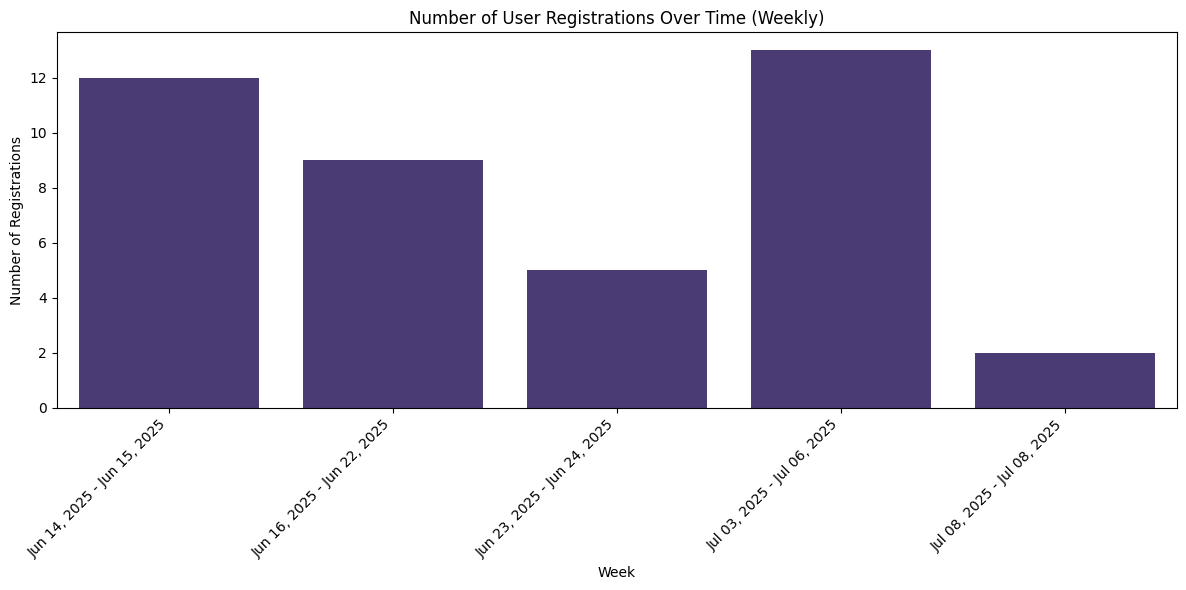
\includegraphics[width=0.85\textwidth]{figures/chapt7/section7.3/BarChart_Contributors.png}
\caption{Weekly counts of new WeCyclePH user registrations, highlighting trends in platform adoption over the deployment period.}
\label{fig:BarChart_ContributorRegistration}
\end{figure}

Over the course of four weeks, a total of 45 users registered on the mobile application. Out of these, 13 cyclists actively contributed ride data, reflecting a moderate but engaged cohort of early adopters.

As shown in Figure~\ref{fig:BarChart_ContributorRegistration}, which presents a bar chart of new user registrations per week, registration activity peaked during the first week, with 10 users signing up, likely influenced by direct participant recruitment and early exposure within targeted communities. A second notable spike occurred during the first week of July, with 8 additional users registering. This uptick is attributed to increased promotional visibility generated by official posts from DLSU's institutional Facebook page and the College of Computer Studies' community group.

These trends suggest that participation was strongly correlated with personal outreach and institutional amplification, reinforcing qualitative feedback that most contributions came from cyclists who were either directly invited or motivated by structured incentives (e.g., equipment trials and test prompts). As discussed in Section~\ref{sec:thematic_analysis_results}, this aligns with interview findings where users stated that they were more likely to try the app when referred by peers or when incentivized to test features such as automated annotations.

Overall, while the contributor base was modest in size, it demonstrated meaningful engagement during the critical early-phase deployment. The following sections explore how this group interacted with the platform and what data they produced in terms of both ride logging and annotation behaviors.

\subsection{Ride Data Summary}

This section presents the quantitative cycling data collected through WeCyclePH, reflecting both the diversity and behavior of early users across a variety of environments. Over the four-week period, the application successfully logged a total of 58 unique cycling sessions, representing a meaningful dataset for assessing usage trends and early system performance. The average distance per ride was 11.7 kilometers, suggesting a mix of short urban commutes and longer exploratory or recreational trips. In total, these rides amounted to approximately 47 hours of recorded cycling activity.

\begin{figure}[H]
\centering
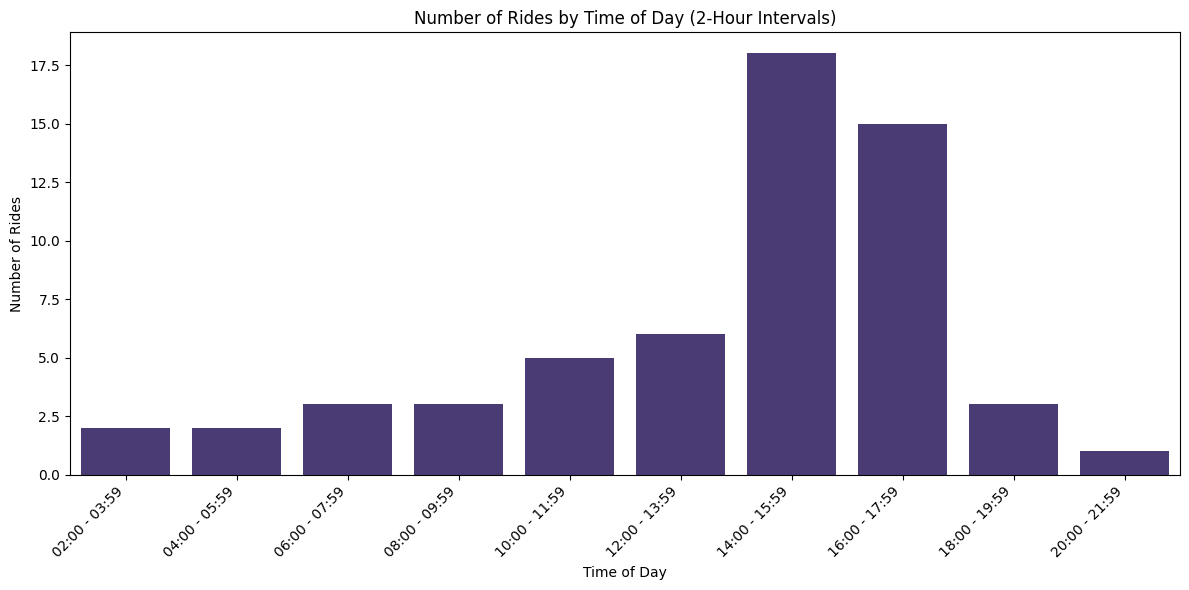
\includegraphics[width=1.0\textwidth]{figures/chapt7/section7.3/RideDataSummary_BarChart_FreqTimeDay.png}
\caption{Distribution of recorded rides by time of day in two-hour intervals, showing patterns in cyclists’ riding activity throughout the day.}
\label{fig:RideDataSummaryt_FreqTimeDay}
\end{figure}

Temporal patterns in the data reveal that the most common riding time fell between 2:00~PM and 6:00~PM, indicating a preference among contributors for afternoon cycling, possibly due to personal schedules or reduced road congestion during this period. As illustrated in Figure~\ref{fig:RideDataSummaryt_RideFreqOverTime}, ride activity was relatively consistent throughout the deployment window, but spikes were observed in the fourth week of June and the first week of July, periods that coincided with increased platform visibility via online promotions and the introduction of data contribution incentives.

\begin{figure}[H]
\centering
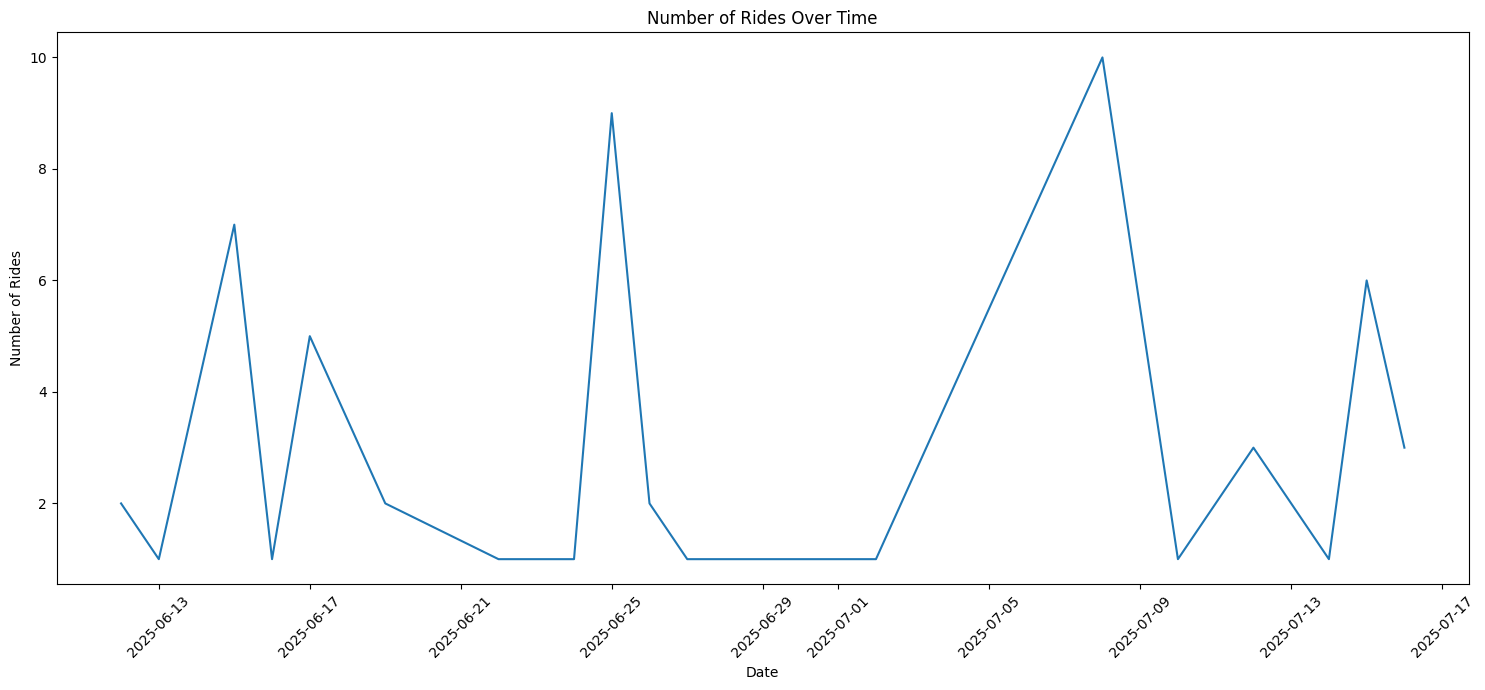
\includegraphics[width=0.85\textwidth]{figures/chapt7/section7.3/RideDataSummary_LineChart_RideFreqOverTime.png}
\caption{Ride counts recorded on the WeCyclePH platform over time, illustrating trends in user activity and data contributions throughout the deployment period.}
\label{fig:RideDataSummaryt_RideFreqOverTime}
\end{figure}

In terms of geographic distribution, Figure~\ref{fig:RideDataSummary_RidesPerRegion} shows that Calabarzon contributed the largest number of rides (26 trips), most of which were submitted by incentivized testers evaluating the machine-generated annotation tool. Metro Manila followed closely with 23 rides, while Zamboanga Peninsula and the Cordillera Region contributed 8 and 1 rides respectively. This spread demonstrates WeCyclePH's ability to reach both urban and provincial contexts, although still skewed toward areas where recruitment efforts were most concentrated.

\begin{figure}[H]
\centering
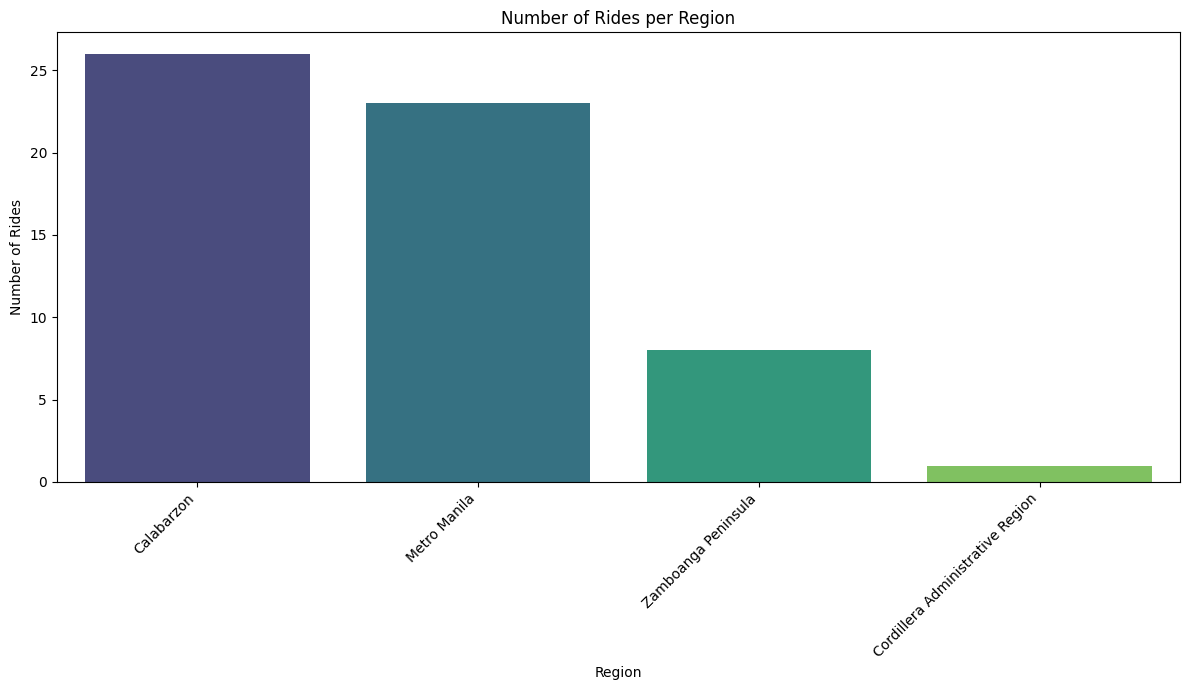
\includegraphics[width=0.85\textwidth]{figures/chapt7/section7.3/RideDataSummary_BarChart_RidesPerRegion.png}
\caption{Frequency of recorded rides by region, illustrating geographic patterns of cycling activity contributed to the WeCyclePH platform within the 4-week collection period.}
\label{fig:RideDataSummary_RidesPerRegion}
\end{figure}

Speed and elevation data, captured through GPS logs, were used to further analyze the performance and consistency of the recording system. Figure~\ref{fig:RideDataSummary_BoxPlot_DistSpeedElev} presents box plots of ride distance, speed, and elevation gain. The average speed recorded was 15.7~kph, with a standard deviation of 5.7~kph, a reasonable range for urban cycling. However, upper outliers (e.g., a maximum speed of 33.1~kph) may indicate hardware-related GPS jitter or data spikes. Similarly, ride elevation values ranged widely, with an extreme maximum of over 1100 meters, likely due to GPS error or signal loss in mountainous or obstructed areas. The minimum recorded distance of 0.06~km reflects test rides or app trials where the ride was logged but not continued.

\begin{figure}[H]
\centering
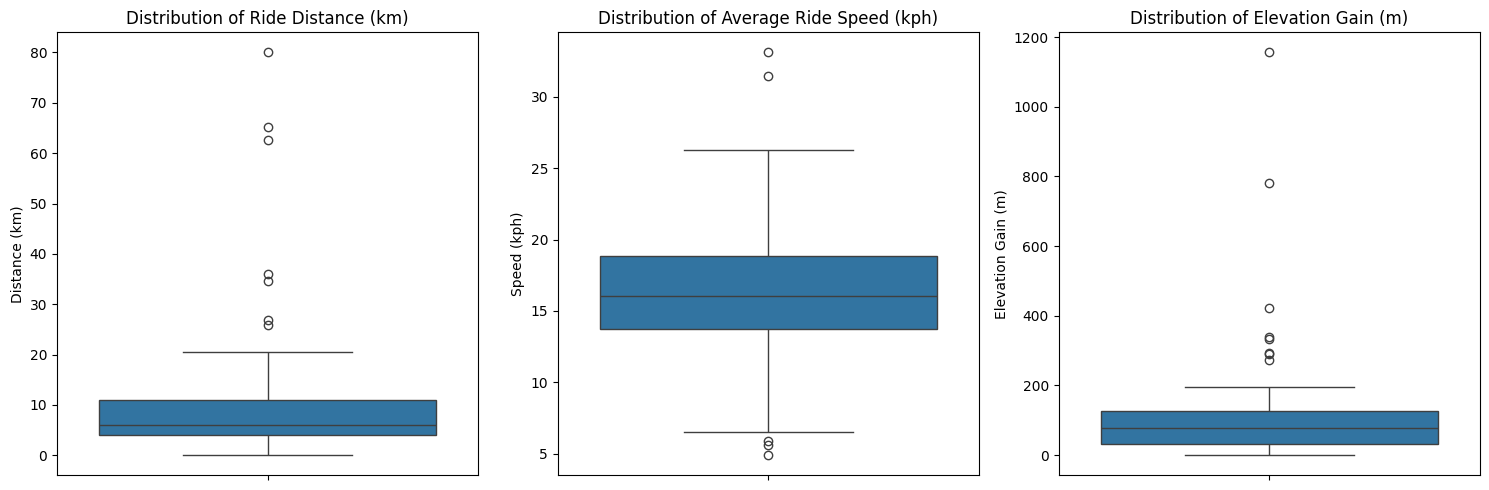
\includegraphics[width=1.0\textwidth]{figures/chapt7/section7.3/RideDataSummary_BoxPlot_DistSpeedElev.png}
\caption{Distributions of ride distance, average speed, and elevation gain across all recorded rides, providing an overview of the variability in cycling activity on the WeCyclePH platform.}
\label{fig:RideDataSummary_BoxPlot_DistSpeedElev}
\end{figure}

All but one of the rides were recorded through the mobile application, with only a single contribution uploaded via a GPX file, highlighting that early users overwhelmingly preferred the built-in GPS logging feature. Additionally, 11 rides included video footage, all of which came from incentivized participants using the experimental auto-annotation system. This reinforces qualitative findings that media contribution tends to increase when barriers are reduced and users are encouraged or equipped to contribute richer data.

Together, these ride logs offer foundational insight into user behavior, spatial coverage, and potential data quality issues. The following section explores how users layered subjective information onto these rides through manual annotations.

\subsection{User Annotations Analysis}

Beyond GPS and video tracking, WeCyclePH allowed users to manually annotate their rides with observations about road conditions, hazards, and infrastructure features. These subjective inputs provided deeper contextual value to the data, capturing details that automated tools alone might miss. During the deployment period, a total of 181 annotations were submitted, distributed across 21 rides, and contributed by 6 unique users. This volume of annotations, relative to the number of rides, suggests that a core group of testers actively participated in enriching their recorded sessions with meaningful insights.

\begin{figure}[H]
\centering
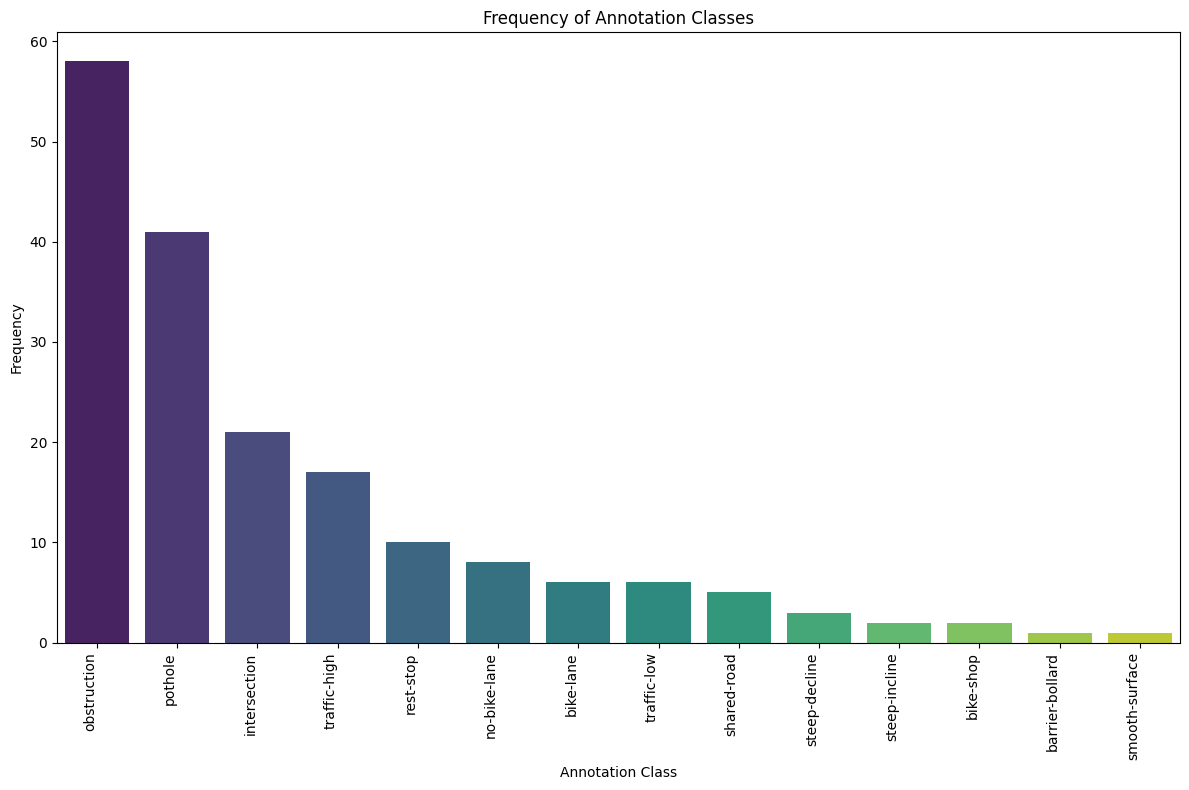
\includegraphics[width=1.0\textwidth]{figures/chapt7/section7.3/UserAnnotations_BarChart_FreqAnnotClasses.png}
\caption{Frequency of annotations by class, showing the distribution of reported cycling experiences and road conditions contributed to the WeCyclePH platform in descending order.}
\label{fig:UserAnnotations_FreqAnnotClasses}
\end{figure}

Annotations were categorized into three broad classes: Hazards, Points of Interest, and Infrastructure Feedback. As shown in Figure~\ref{fig:UserAnnotations_FreqAnnotClasses}, the four most common types of hazards reported were obstructions (58) and bogs (41), followed by intersections (21) and high-traffic areas (17). Rest stops reached a count of 10, but the remaining classes captured less frequent observations, such as roads with bike lanes and no bike lanes, steep inclines and declines, and smooth or rough surfaces. This distribution highlights users' focus on safety-critical features and environmental constraints while navigating urban and semi-urban areas.

\begin{figure}[H]
\centering
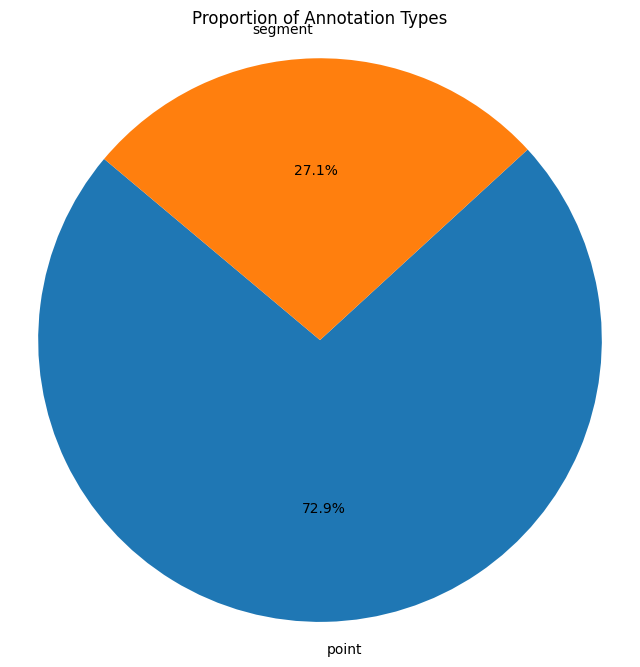
\includegraphics[width=0.6\textwidth]{figures/chapt7/section7.3/UserAnnotations_PieChart_AnnotTypeProportions.png}
\caption{Proportions of point-based and segment-based annotations contributed to the WeCyclePH platform, showing a user preference for logging discrete hazards over extended road conditions.}
\label{fig:UserAnnotations_AnnotTypeProportions}
\end{figure}

A breakdown of annotation styles shows a strong preference for point-based annotations, which represented 72. 9\% of all entries, compared to 27.1\% for segment-based annotations (Figure~\ref{fig:UserAnnotations_AnnotTypeProportions}). Point annotations typically marked a single location (e.g. a pothole or construction site), while segments were used to describe conditions along a stretch of road (e.g., a long incline or poorly maintained lane). This preference suggests that most users found it easier and more intuitive to log discrete hazards, which is consistent with the usability feedback collected during the beta phase.

\begin{figure}[H]
\centering
\begin{minipage}{0.49\textwidth}
  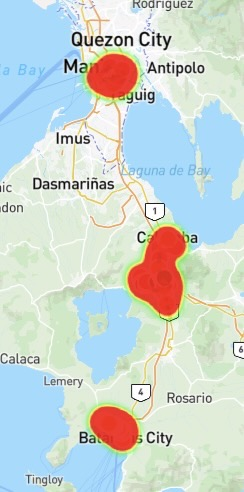
\includegraphics[width=\linewidth]{figures/chapt7/section7.3/UserAnnotations_Heatmap_Whole.jpeg}
\end{minipage}%
\hfill
\begin{minipage}{0.49\textwidth}
  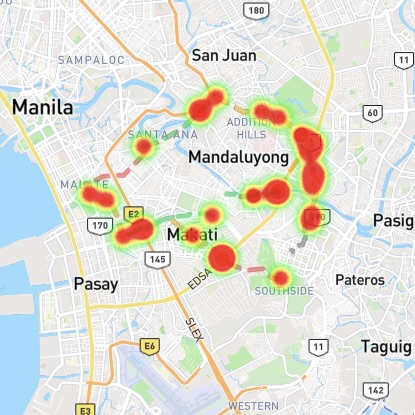
\includegraphics[width=\linewidth]{figures/chapt7/section7.3/UserAnnotations_Heatmap_Manila.jpeg}
  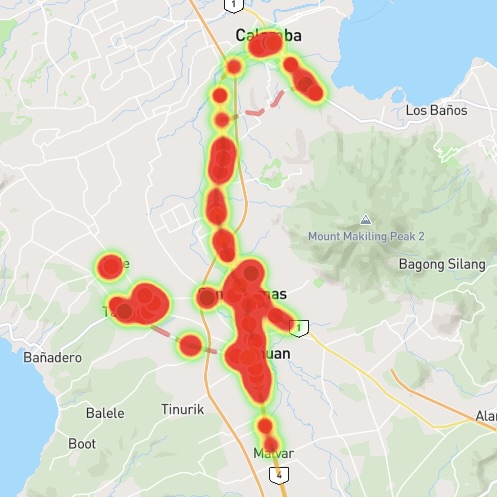
\includegraphics[width=\linewidth]{figures/chapt7/section7.3/UserAnnotations_Heatmap_Batangas.jpeg}
\end{minipage}
\caption{Geographical distribution of user-submitted annotations, highlighting high-density clusters in Metro Manila and Batangas, particularly along routes such as Shaw Boulevard, Maharlika Highway, and select areas in Buendia and Makati.}
\label{fig:UserAnnotations_AnnotHeatMap}
\end{figure}

Geographically, annotation density was highest in Metro Manila and Batangas, particularly along high-use routes such as Shaw Boulevard, Maharlika Highway, select areas in Buendia and Makati. As visualized in Figure ~\ref{fig:UserAnnotations_AnnotHeatMap}, these regions exhibited concentrated activity related to obstructions and high-traffic encounters. Temporal analysis of annotation timestamps further revealed that afternoon rides generated more hazard reports, possibly due to increased traffic congestion.

The quality and richness of the annotation data were further enhanced through sentiment tagging and media contributions. Out of the 181 total annotations, 31 included sentiments, most of which were associated with routes in Metro Manila. These sentiments provided valuable insights into cyclists' emotional responses to different road conditions. Additionally, 83 annotations included media attachments, such as photographs or short video clips, which were particularly useful for validating hazard types and supporting downstream computer vision tasks.

% TODO Image of submission with picture and sentiments
\begin{figure}[H]
\centering
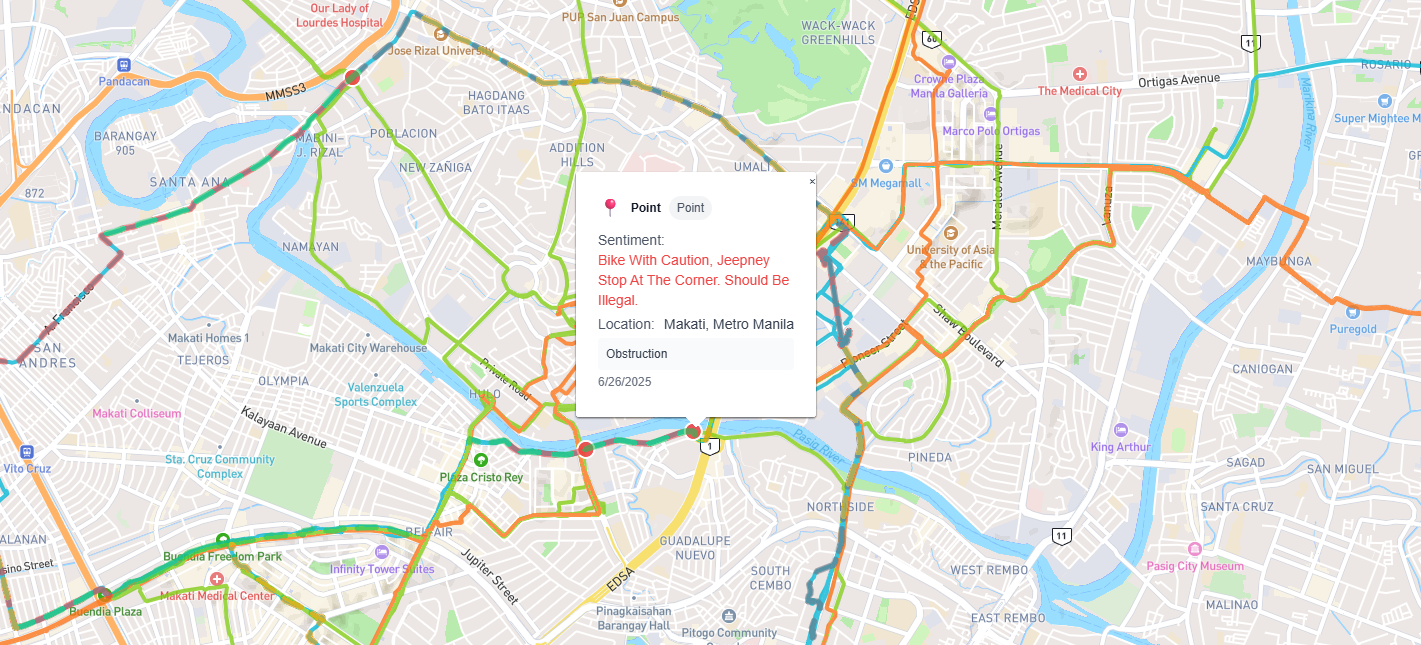
\includegraphics[width=0.85\textwidth]{figures/chapt7/section7.3/UserAnnnotations_Point.png} 
\caption{Screenshot of the annotation interface in the WeCyclePH web application, showing an example submission with a geotagged hazard report and predefined category selection.}
\label{fig:UserAnnotations_ui_screenshot}
\end{figure}

Taken together, these findings highlight that users were not only willing to contribute annotations but did so with a degree of intentionality and attention to detail. While overall annotation participation was limited to a small subset of testers, their contributions illustrate the value of subjective data in building a nuanced and actionable cycling dataset.


\subsection{Machine-Generated Annotations via Instance Segmentation}

To reduce the burden of manual tagging and improve the richness of contributed ride data, WeCyclePH integrated a rule-based annotation system powered by instance segmentation. The system automatically generates semantic tags from model detections on uploaded videos, supporting both infrastructure mapping and cyclist safety analysis. This section discusses the system's observed behavior, annotation distribution, and user sentiment toward the feature.

\subsubsection*{Inference Output and Annotation Generation}

A total of 8 user-contributed videos were processed, resulting in 1,552 frames sampled at 5-second intervals. From these frames, the instance segmentation model generated 1,346 valid object detections. The most frequently detected object classes were \texttt{car} (515), \texttt{bike\_lane} (326), and \texttt{truck} (234), while classes such as \texttt{barrier} (12), \texttt{tricycle} (3), and \texttt{bus} (1) were detected infrequently.

Using the predefined logical rules outlined in Table~\ref{tab:annotation_logic}, the inference results yielded a total of 39 machine-generated annotations. These were distributed across the following tag types:

\begin{table}[H]
\centering
\begin{tabular}{|l|c|}
\hline
\textbf{Class} & \textbf{Number of Detections} \\
\hline
\texttt{car}         & 515 \\
\texttt{bike\_lane}  & 326 \\
\texttt{truck}       & 234 \\
\texttt{person}      & 111  \\
\texttt{jeepney}     & 94 \\
\texttt{motorcycle}     & 33 \\
\texttt{bicycle}    & 16 \\
\texttt{barrier}     & 12 \\
\texttt{tricycle}    & 3 \\
\texttt{bus}         & 1 \\
\hline
\textbf{Total Frames Processed} & 1,552 \\
\textbf{Total Detections}       & 1,345 \\
\hline
\end{tabular}
\caption{Instance segmentation inference results from eight processed cycling videos, showing the total number of detections per object class and overall detection counts across 1,552 analyzed frames.}
\label{tab:inference_stats}
\end{table}

\subsubsection*{Annotation Distribution Across Videos}
Table~\ref{tab:annotation_distribution} presents the breakdown of annotation types per video. Videos are anonymized as Video A through H. The table includes total annotation counts and per-type frequency per video.

\begin{table}[H]
\centering
\setlength{\tabcolsep}{4pt} % Reduce horizontal padding
\renewcommand{\arraystretch}{1.1} % Adjust row height
\begin{tabular}{|l|c|c|c|c|c|c|c|c|c|}
\hline
\textbf{Category} & \textbf{A} & \textbf{B} & \textbf{C} & \textbf{D} & \textbf{E} & \textbf{F} & \textbf{G} & \textbf{H} & \textbf{Total} \\
\hline
Total Annotations & 3 & 3 & 6 & 5 & 5 & 7 & 7 & 3 & 39 \\
\texttt{Obstruction} & 1 & 0 & 2 & 1 & 0 & 4 & 5 & 0 & 13 \\
\texttt{Low-to-No Traffic} & 1 & 1 & 1 & 1 & 1 & 1 & 1 & 1 & 8 \\
\texttt{Bike Lane} & 1 & 0 & 1 & 1 & 1 & 1 & 1 & 1 & 7 \\
\texttt{No Bike Lane} & 0 & 1 & 1 & 1 & 1 & 1 & 0 & 1 & 6 \\
\texttt{High Traffic} & 0 & 1 & 0 & 1 & 1 & 0 & 0 & 0 & 3 \\
\texttt{Shared Road} & 0 & 0 & 1 & 0 & 1 & 0 & 0 & 0 & 2 \\
\hline
\end{tabular}
\caption{Distribution of machine-generated annotation types across eight cycling videos (A–H). Each row represents a category, and each column (A–H) shows the count for that video.}
\label{tab:annotation_distribution}
\end{table}


As shown, \texttt{Obstruction} was the most frequently generated tag, appearing in 6 out of 8 videos and accounting for 28\% of all annotations. Conversely, \texttt{Shared Road} appeared only twice, indicating either stricter rule criteria or underrepresentation of that context in the data. 

\subsubsection*{User Feedback and Perceived Value}

User interviews indicate that the automation of annotations was widely seen as a beneficial addition, particularly in light of the safety constraints experienced while riding. Cyclists highlighted that stopping to annotate mid-ride introduced risk and discomfort:

\begin{quote}
\textit{"What's only hard for me is that I need to stop always to report something... But I can report and take pictures while moving... the only hard part is stopping."} -- P2
\end{quote}

The automated approach was seen as a safer, more efficient alternative:

\begin{quote}
\textit{"Definitely, it's really convenient... it removes all of those inconveniences especially that your safety is not compromised."} -- P2
\end{quote}

Some users stated that automation would make them more willing to upload longer videos, knowing that the system could assist in annotation:

\begin{quote}
\textit{"Yes, I will definitely rather upload videos more if I have this tool because I feel like it's that convenient."} -- P2
\end{quote}

Others acknowledged that while the feature was useful, adoption might still vary:

\begin{quote}
\textit{"Still 50/50, maybe for those who can, yes."} -- P3
\end{quote}

There was also enthusiasm for seeing these tags reflected in shared maps and for their potential impact:

\begin{quote}
\textit{"You know, seeing these many obstructions, potholes, in the map, it's very significant to us cyclists."} -- P2
\end{quote}

\subsubsection*{Implications}

The distribution of annotation types reflects both model capabilities and contextual frequency in urban cycling environments. Annotations such as \texttt{Obstruction} are likely to be triggered by frequent, visually distinct objects such as cars or motorcycles. Meanwhile, annotations requiring more nuanced or combined detections, such as \texttt{Shared Road}, occurred less often.

User feedback supports the integration of automatic annotation as an assistive feature, not only for reducing the effort of manual annotations but also for enabling broader participation from cyclists who ride in more challenging or high-traffic contexts. However, limitations remain, including:
\begin{itemize}
    \item Model performance on low-frequency classes (e.g., \texttt{barrier}, \texttt{bus}) may underrepresent certain conditions.
    \item The temporal sampling rate (1 frame every 5 seconds) may miss short-lived features.
    \item Media upload workflows remain semi-manual, presenting barriers to contribution.
\end{itemize}

\section{Discussion and Design Implication}

\subsection{Evaluating Data Quality and Dataset Representativeness}

A core concern of any crowdsourced dataset is the question of quality: \textit{How can we say that we were able to gather quality data?} This section provides a critical evaluation of the data collected through the WeCyclePH platform, examining not just its volume but its diversity, spatial distribution, annotation integrity, and alignment with real-world cycling conditions.

\subsubsection{Contributor Profile and Participation Patterns}

The dataset was built through voluntary contributions from a diverse pool of cyclists. In total, \textbf{45 users} created accounts and joined the platform, with \textbf{13 users} actively contributing GPS-tracked rides and annotations. Recruitment occurred organically through social media outreach and peer networks, including cycling advocacy groups and student communities. Contributors include daily commuters, students, recreational cyclists, and urban mobility advocates.

While contributions came from varied demographics, data skewed toward individuals who regularly cycle as a primary mode of transportation—particularly in urban contexts. This is consistent with the observed density of rides in metropolitan areas (see Figure~\ref{fig:UserAnnotations_AnnotHeatMap}). Recreational cyclists were also represented, but less frequently.

\subsubsection{Volume and Composition of the Dataset}

The dataset comprises \textbf{58 unique rides}, \textbf{181 manual annotations},\textbf{34 machine-generated annotations}. Each ride is processed into multiple directionally consistent segments, with derived metrics such as average speed, distance, elevation gain, and annotation associations. Short or incomplete rides under 10 meters were filtered out as outliers to maintain baseline data integrity.

The dataset was designed not only for volume but for variety. Riders traversed different types of roads—from protected bike lanes to shared roads and informal paths. Although there was no enforced quota or minimum contribution requirement, the ride data collectively spans a meaningful diversity of road conditions.

\begin{figure}[H]
\centering
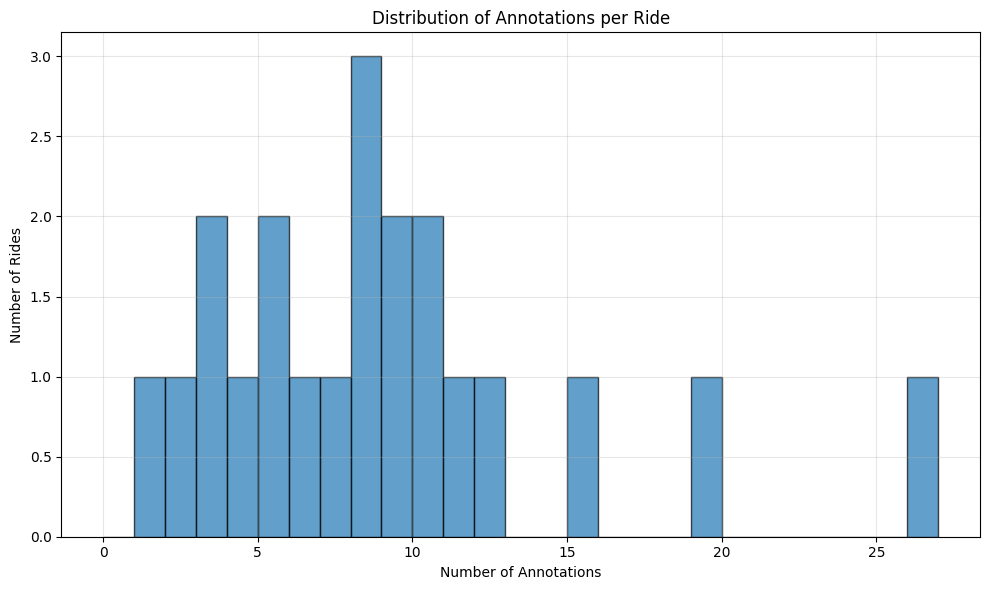
\includegraphics[width=0.85\textwidth]{figures/chapt7/section7.4/Histogram_AnnotationsPerRide.png}
\caption{Histogram showing the distribution of annotations per ride in the WeCyclePH dataset, indicating how frequently cyclists submitted reports during individual trips.}
\label{fig:Histogram_Annotations_Per_Ride}
\end{figure}

\subsubsection{Geographic Distribution and Coverage}

Although WeCyclePH was open to users across the Philippines, contributions clustered in specific geographic regions. The vast majority of rides were recorded in \textbf{Metro Manila} and \textbf{Batangas}, followed by a smaller number of rides from \textbf{Baguio} and \textbf{Zambales}. While this reflects where cyclists are more densely concentrated or more tech-connected, it also introduces regional biases in the dataset's representativeness.

We acknowledge that some known underserved or rural areas were not captured. However, the platform's openness, mobile-first deployment, and accessible recording interface enabled decentralized data collection across four provinces.

\begin{figure}[H]
\centering
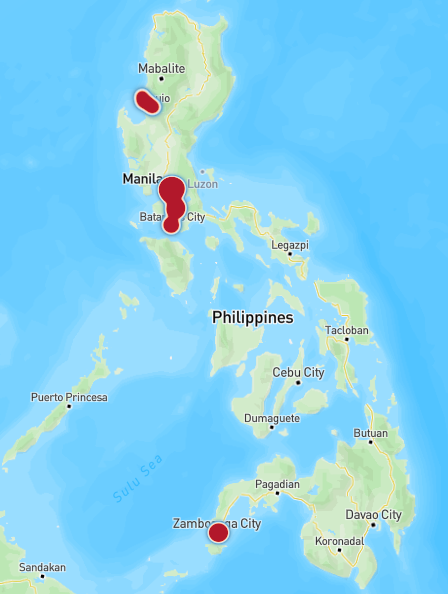
\includegraphics[width=0.85\textwidth]{figures/chapt7/section7.4/Heatmap_Country_Coverage.png}
\caption{Heatmap visualizing the geographical coverage of recorded GPS traces collected through WeCyclePH during the public beta period, highlighting concentration of contributions in Metro Manila, Batangas, Baguio, and Zambales, with limited representation from rural or underserved areas}
\label{fig:Heatmap_country_coverage}
\end{figure}

\subsubsection{Annotation Usage and Integrity}

One of the central goals of the WeCyclePH dataset was to not only capture geospatial ride traces, but to allow cyclists themselves to document the context of their experience through structured annotations. These annotations serve as a rich qualitative layer describing road quality, infrastructure, and subjective perceptions such as comfort or danger.

Over the course of the data collection period, a total of \textbf{181 manual annotations} were submitted across 58 rides. Each annotation was assigned one of 17 predefined labels, and users had the option to attach media, write descriptive sentiments, and apply additional tags. These annotations were associated with specific GPS coordinates in their respective rides, either through single-point tags (e.g., noting a pothole at a specific intersection) or short path segments (e.g., describing a stretch of shared road or poor surface). We were also able to process user-submitted videos into 39 machine-generated annotations, 34 of which were mapped to their respective rides.

\vspace{0.3cm}
\noindent\textbf{Annotation Label Distribution.}
Two annotation types stand out in terms of usage: \texttt{obstruction} (n=58) and \texttt{pothole} (n=41). Together, these account for more than half of all submitted annotations, suggesting a high salience of road hazards in cyclist perception. Users frequently used the \texttt{obstruction} label to describe parked vehicles, construction equipment, debris, or vendors blocking bike lanes. Meanwhile, \texttt{pothole} annotations often referred to deep and dangerous pavement defects, which were also corroborated through uploaded photos and video footage in many cases.

Other frequently used labels include \texttt{intersection}, \texttt{traffic-high}, and \texttt{rest-stop}, which indicate not only the types of road features that cyclists encountered but also the decisions they made during navigation (e.g., stopping, changing speed, or rerouting).

\texttt{no-bike-lane}, \texttt{bike-lane}, and \texttt{shared-road} were also used, albeit less frequently, to capture the infrastructure context in which the ride occurred. This reflects the fact that some areas had mixed or ambiguous infrastructure, which might not always be noticed or tagged consistently by all users. Other labels such as \texttt{steep-incline}, \texttt{smooth-surface}, or \texttt{barrier-bollard} appeared infrequently, potentially due to underreporting or users' focus on more disruptive or negative road elements.

\vspace{0.3cm}
\noindent\textbf{Annotation Comprehension and Interface Usability.}
User interviews conducted as part of our evaluation protocols revealed that contributors generally understood the labeling schema well. Cyclists did not report confusion regarding the predefined annotation labels. The annotation interface, which included icons, descriptions, and sample images, was found to be intuitive by both student users and experienced cyclists.

Although no formal validation mechanism was embedded into the system (e.g., community upvoting, expert reviews), informal moderation was performed. Researchers manually reviewed a random sample of rides, especially those that included video footage, to assess whether annotations aligned with visible road conditions. These audits found a high degree of alignment between annotation labels and the recorded context.

\vspace{0.3cm}
\noindent\textbf{Annotation Length and Depth.}
Most annotations consisted of a single point tagged along a ride, though the dataset supports both point- and segment-based annotations. The majority of user-generated annotations did not include detailed free-text sentiments or media uploads, likely due to the optional nature of those fields. However, some users did upload photos and videos, which provided additional context during qualitative review (see Table~\ref{tab:representative_annotations}).

\begin{table}[H]
\centering
\begin{tabular}{|p{3cm}|p{7cm}|p{3.5cm}|}
\hline
\textbf{Label} & \textbf{Sentiment} & \textbf{Media} \\
\hline
obstruction & None & 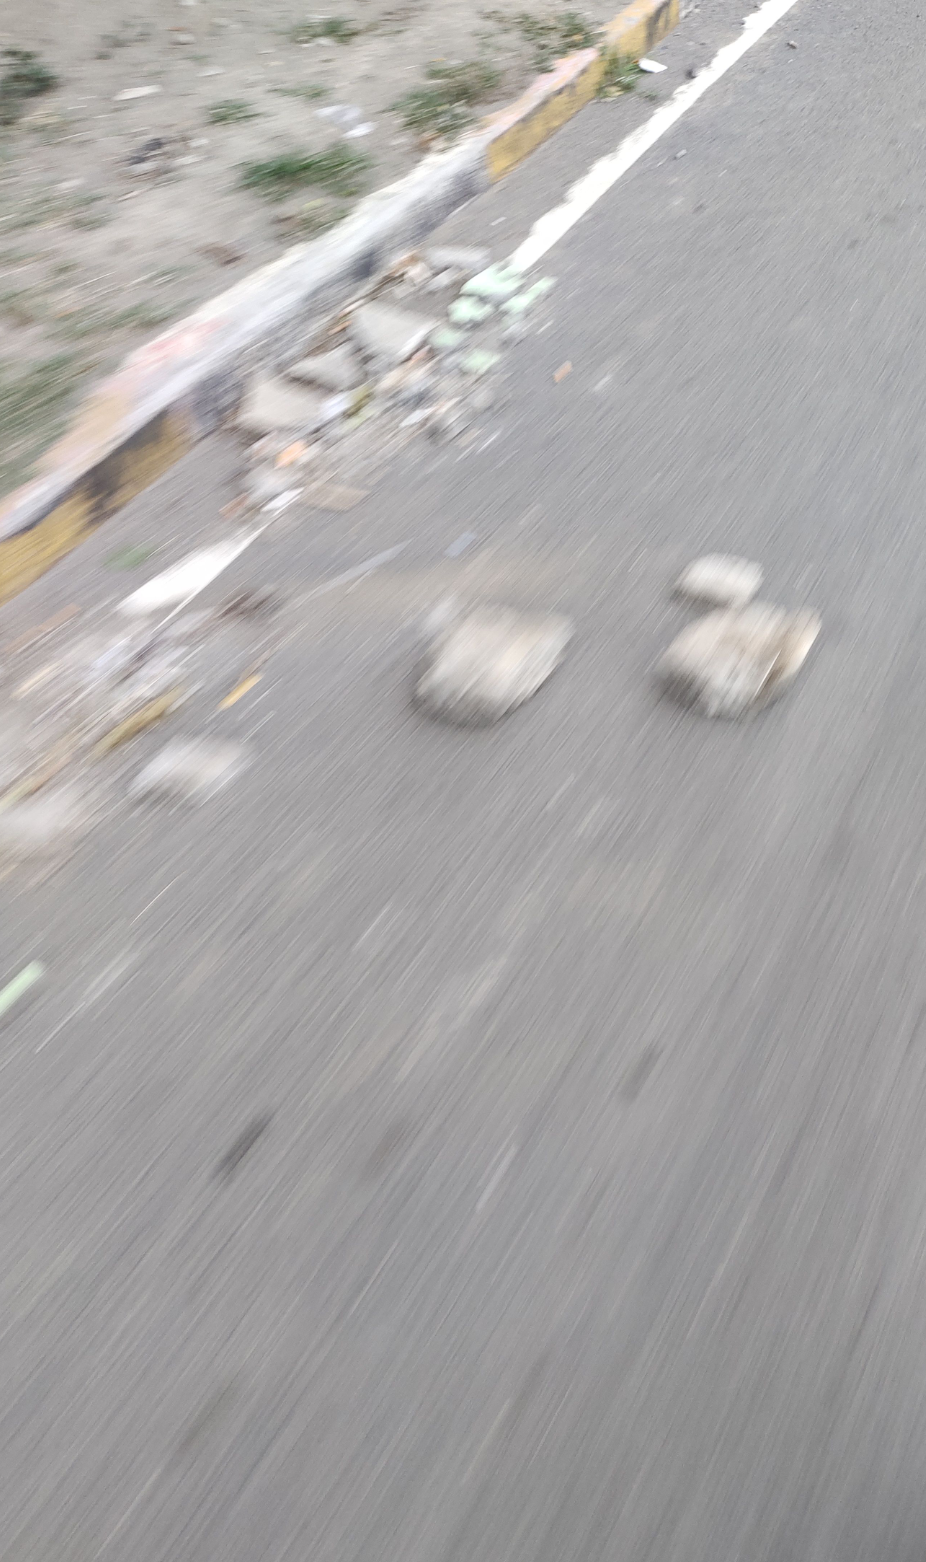
\includegraphics[width=3cm]{figures/chapt7/section7.4/UserAnnotation_Example_Obstruction.png} \\
\hline
pothole & None & 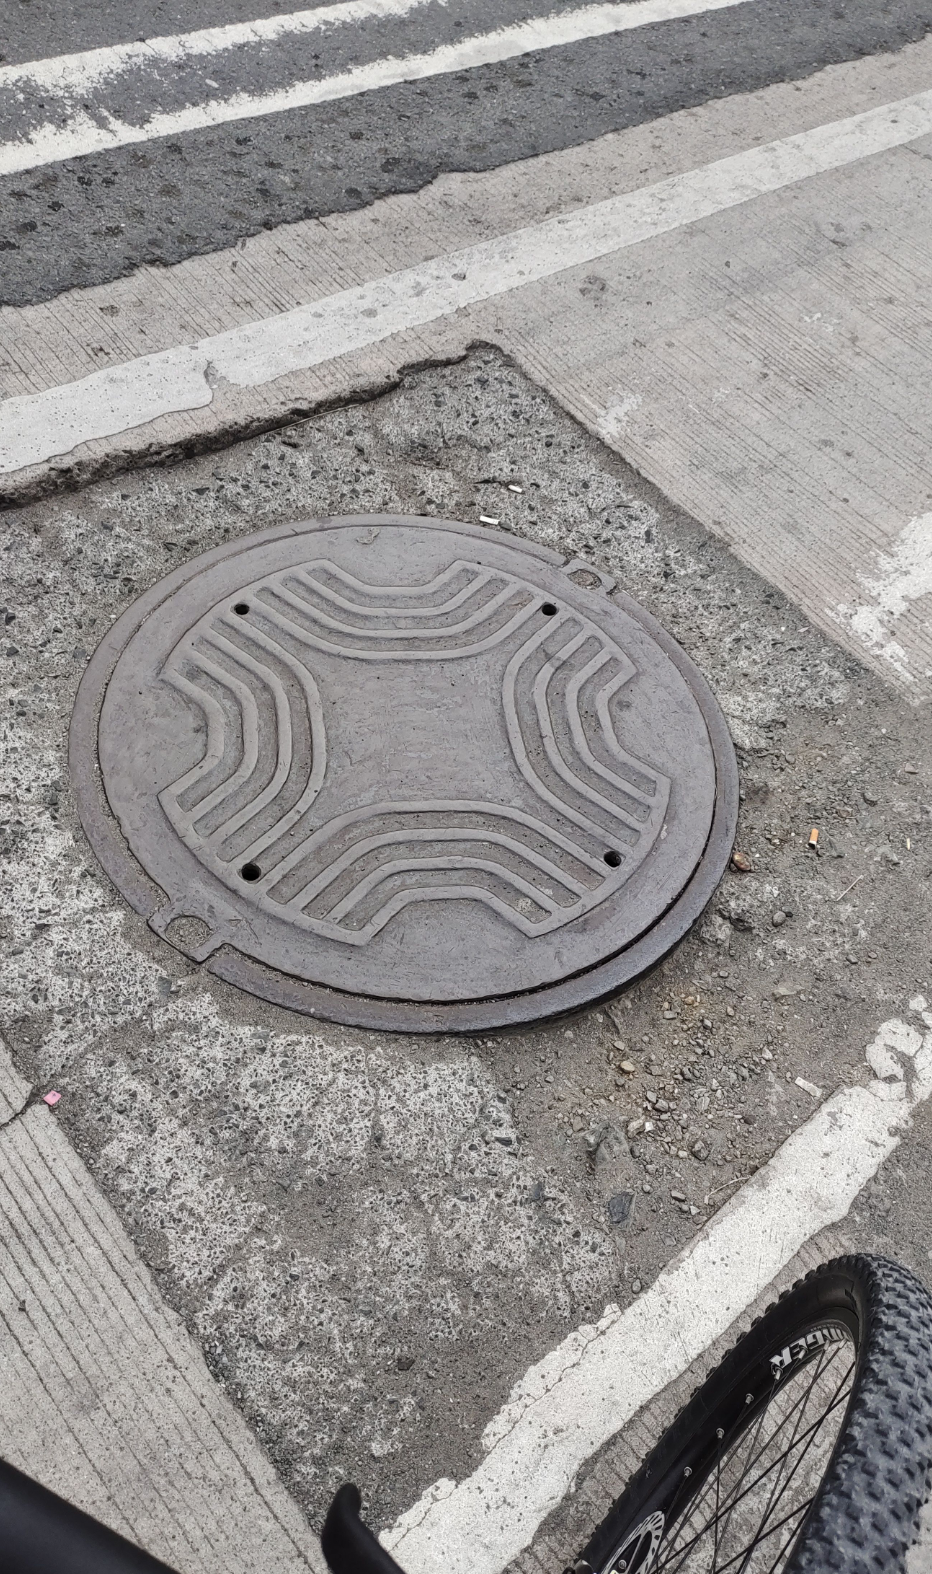
\includegraphics[width=3cm]{figures/chapt7/section7.4/UserAnnotation_Example_Pothole.png} \\
\hline
intersection & None & 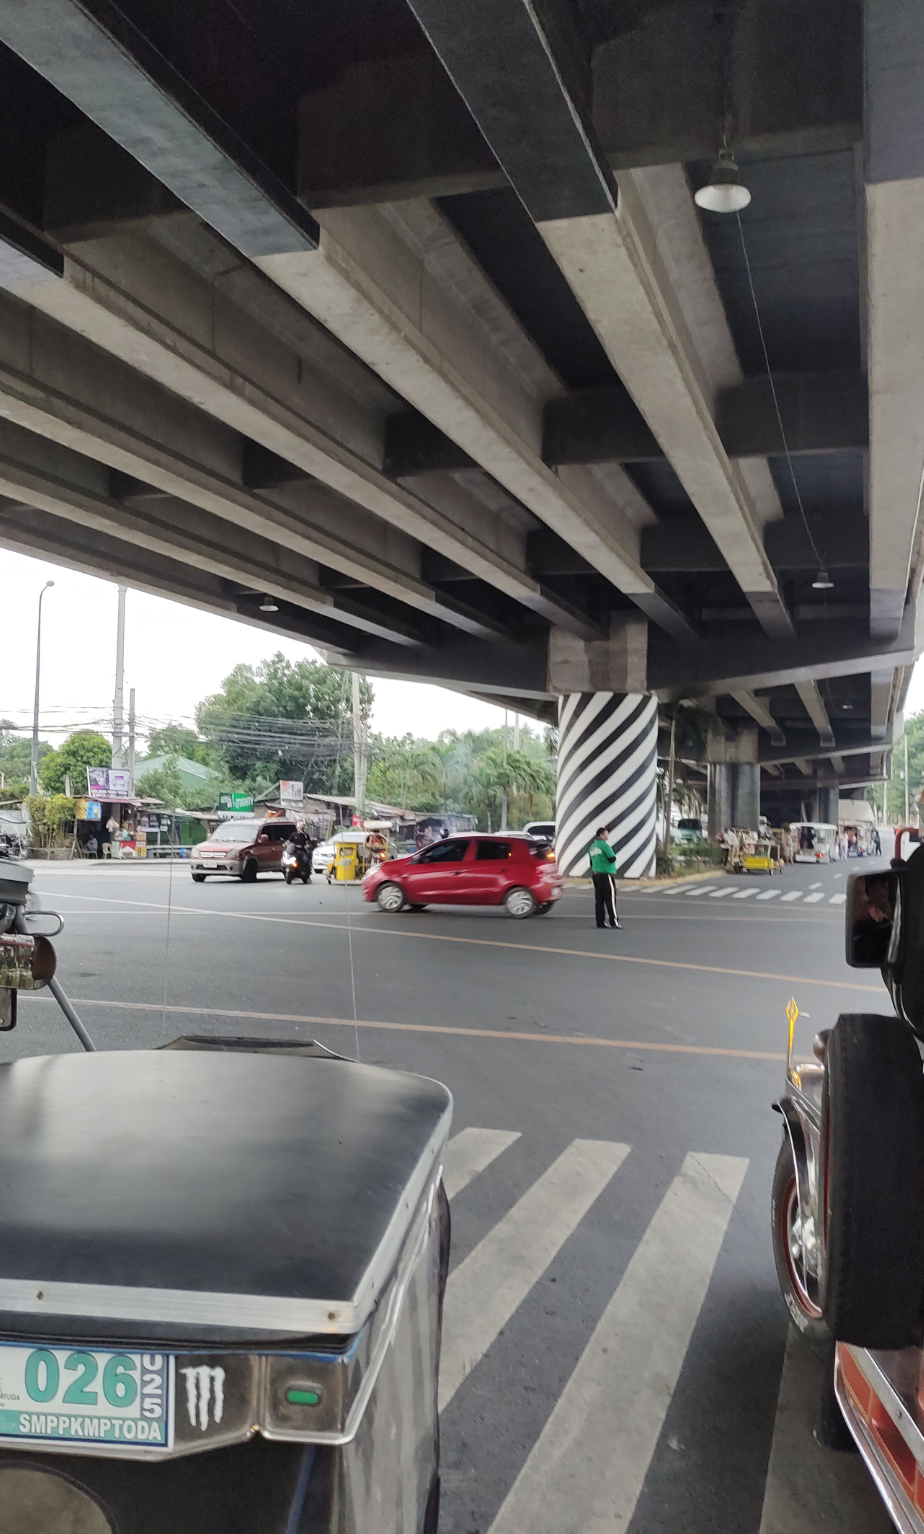
\includegraphics[width=3cm]{figures/chapt7/section7.4/UserAnnotation_Example_Intersection.png} \\
\hline
bike-lane & \textit{Ayala bike lane is private, Gil Puyat is DOTr project} & None \\
\hline
traffic-high & \textit{U need to merge and make left merge to go to BGC. Ingat lagi sa pakaliwang merge, kasabayan mo mabibilis rin. Use hand signals and exercise caution.} & None \\
\hline
\end{tabular}
\caption{Sample user annotations with sentiment and attached media}
\label{tab:representative_annotations}
\end{table}


\vspace{0.3cm}
\noindent\textbf{Summary.}
Overall, user annotations reflected high-quality engagement, with frequent use of infrastructure- and hazard-related labels that align with known issues in Philippine road networks. The prevalence of \texttt{obstruction}, \texttt{pothole}, and \texttt{intersection} tags highlights both the value of crowd insight and the gaps in urban cycling infrastructure. Though some annotation classes were underutilized, this reflects user priorities and perception rather than system limitations. The annotation system served not only as a tagging tool, but also as a mechanism for cyclists to express lived mobility conditions with spatial precision.

\subsubsection{Technical Quality: GPS, Metrics, and Processing}

Technical issues are a common concern in GPS-based mobile sensing. Contributors reported occasional GPS drift, UI lags, and upload disruptions. However, the dataset design includes robust post-processing logic to address such inconsistencies. For instance:

\begin{itemize}
\item Ride-level metrics (e.g., speed, distance) are recomputed from the raw point traces to correct for any logging inaccuracies.
\item Segments are computed based on a bearing-difference heuristic, with manual inspections to assess over-segmentation or under-segmentation.
\item Elevation gain is derived from smoothed point-to-point elevation deltas to avoid distortions from barometric spikes or missing values.
\end{itemize}

The integrity of this recomputation process was verified by comparing original device-calculated values with recomputed ones on all crowdsourced rides.

\subsubsection{Limitations and Observed Biases}

Despite its depth, the dataset exhibits several limitations:

\begin{itemize}
\item \textbf{Urban bias}: Dense contributions in Metro Manila and Batangas may over-represent well-connected road networks.
\item \textbf{Low density in rural areas}: No significant contributions were recorded from under-served provinces or informal cycling routes.
\item \textbf{Temporal granularity gaps}: Since annotations were added post-ride, some users may have forgotten exact timestamps or skipped locations entirely.
\item \textbf{Sparse repeat rides}: Few users contributed multiple rides in the same area, limiting longitudinal analysis of changing road conditions.
\end{itemize}

Future expansions of the dataset could incorporate active prompts for annotation during rides, incentives for repeated contributions, and community-driven quality verification.

\subsubsection{Toward a Definition of “Data Quality” in Urban Cycling Contexts}

When considering what constitutes "quality" in urban cycling data, especially data that is community-generated, we must look beyond traditional metrics like volume, completeness, and consistency. In our context, we define data quality along five interdependent dimensions:

\begin{itemize}
\item \textbf{Relevance}: The dataset must contain content that matters to cyclists—this includes tags for bike infrastructure, physical hazards, and emotional responses to the environment. Our data reflects this with high counts of obstruction and pothole annotations and frequent reports of intersections and high-traffic areas.

\item \textbf{Interpretability}: The dataset must be understandable to both human and machine agents. In our case, all annotations follow a standardized schema and are consistently structured. Users were not confused by the labeling interface, and metadata such as timestamps and location are embedded at the annotation level.

\item \textbf{Diversity}: Quality data should span diverse geographies, rider types, and infrastructure contexts. While our dataset has clear urban bias, it includes both students and regular commuters, and roads ranging from protected bike lanes to informal paths.

\item \textbf{Traceability}: Annotations must be verifiable. In our case, this includes GPS-coordinated tags, ride segment matching, and supporting media like photos and videos. Where video was uploaded, annotation tags could be visually confirmed.

\item \textbf{Reusability}: A quality dataset should be accessible for downstream use. By using GeoJSON and segment-level metadata, our dataset can be ingested by GIS platforms, routing engines, and statistical tools. It is well-structured, machine-readable, and modular.
\end{itemize}

Together, these criteria form a holistic framework for evaluating data quality in cyclist-centric datasets. Our pipeline may lack formal validation layers or crowd moderation, but its design intentionally elevates subjective, first-person cycling perspectives. The resulting data is structured and rich with context—qualities that support reuse in both research and advocacy workflows.

\subsubsection{Summary}

This section has evaluated the dataset from multiple perspectives-volume, participation, spatial coverage, annotation clarity, and technical reliability. While areas for improvement remain, the current version demonstrates that a lightweight, community-powered data collection pipeline can yield rich, analyzable insights about cyclist experience.

As our contributors, the cyclists, shape the content, patterns, and granularity of this dataset, the result is the evidence of cyclist mobility.

\subsection{Assessing User Engagement and Data Contribution Behavior}

\subsubsection{Motivation for Contribution}
Initial user engagement data revealed that many cyclists were motivated by a combination of altruistic, personal, and curiosity-driven factors. The primary motivation for contributing data to \textit{WeCyclePH} stemmed from users' sense of community engagement and social good. Several participants expressed a strong desire to help others by identifying road hazards and promoting cycling safety. 

For instance, P3, a commuter cyclist, shared, \textit{``Contributing here made me feel like I was able to offer some help, and that's coming from someone who's not really active in social activities.''} This quote reflects a key motivational theme: users who believed they were contributing to a larger cause were more likely to engage consistently with the platform. The sense of contribution to the community emerged as a significant driver of continued participation.

This sentiment was supported by the UEQ results, particularly the high score in the \textit{Stimulation} scale (\textbf{2.19}), which reflects user excitement, motivation, and interest in using the application. Furthermore, the item-level mean score for ``interesting'' and ``motivating'' both exceeded +2.5, underscoring the emotional engagement many users experienced while using the platform. This suggests that contribution was not merely a task but an enjoyable and intrinsically rewarding activity.

While intrinsic motivation was a powerful driver, some users were also initially drawn to \textit{WeCyclePH} by external incentives or social referrals. Even for these users, the sense of belonging to a larger community played a crucial role in sustaining their interest. As P4, who discovered \textit{WeCyclePH} through a referral, stated, \textit{``The annotation feature made me feel good to contribute, like knowing that I was able to give something that will be shown in the map, feels nice to know about.''} 

Similarly, P2 mentioned, \textit{``I think contributing to WeCyclePH is enjoyable and fulfilling. Because I feel like I'm helping the local biking community, the feeling of the collaborative effort made it fulfilling to contribute.''} These responses emphasize that while external incentives may initiate user participation, the sense of belonging and the feeling of contributing to a community are essential for sustained engagement.

This was further corroborated by the \textit{Hedonic Quality} score (\textbf{2.13}) from the UEQ, which represents emotional satisfaction and community enjoyment. High scores in items like ``supporting something valuable'' and ``engaging'' suggest that users saw their contributions as meaningful, not only functionally but also socially. Moreover, \textbf{85\%} of questionnaire respondents marked ``contributing to community safety'' as an important or extremely important factor when asked about their motivations. This highlights that perceived societal impact, not just individual benefit, was central to why users remained engaged.

Overall, these findings demonstrate that user motivation in \textit{WeCyclePH} was rooted in both internal values and collective identity. The blend of intrinsic enjoyment, civic contribution, and social visibility sustained long-term participation and positioned the app as more than just a tool, it became a platform for community advocacy and empowerment.

\subsubsection{Existing Barriers for Contribution}

Despite strong intrinsic motivations to contribute, several technical barriers discouraged regular use of the app, particularly around the annotation process and media uploads. The most notable challenge identified by users was the difficulty of annotating during rides. Cyclists often expressed concerns about safety and convenience when required to stop, switch apps, or manually tag hazards while riding. The need to stop mid-ride, even briefly, was seen as an interruption that diminished the practicality of the platform. For urban commuters, this issue was particularly significant as they needed to remain focused on traffic and road conditions. As P2 shared, \textit{``What's only hard for me is that I need to stop always to report something. When stopping, I need to worry about hazards like cars in the back or if the area is safe to stop by.''} This sentiment was echoed by several other users, indicating that the interruption in their ride for annotation purposes created a barrier to continuous and safe use.

This concern is further reflected in the User Experience Questionnaire (UEQ) results, where the \textit{Efficiency} scale scored a relatively modest \textbf{1.63}. This suggests that although users appreciated the app's basic functionality, they found specific tasks, such as annotation and media uploads, to be cumbersome or disruptive to their natural riding flow.

Another recurring issue was related to the media upload process, specifically when users attempted to upload full ride videos. Many users mentioned that uploading long videos was time-consuming, slow, and data-intensive, especially in areas with poor connectivity or on mobile networks. Upload failures were reported more frequently by users with lower-end devices, which further limited the diversity of media contributions. One participant noted, \textit{``There are times when taking pictures is taking so long,''} while P2 added, \textit{``I took my rides at night, and when I'm trying to take pictures, the picture-taking process is very slow.''} The slowness of media uploads was clearly a barrier, reducing users' willingness to contribute media-rich data. Additionally, some users raised safety concerns when taking photos or videos during their ride. P3 mentioned, \textit{``While I do want to pull out my phone to take a picture, it's kinda risky to do it while biking. So looking at it currently, it's only optimal if you have a second phone or camera.''} This reflects the physical risks associated with using the app while cycling.

Furthermore, P4 expressed frustration with the manual process involved in annotation, stating, \textit{``When you are manually annotating, you need to account for quite a handful of things, like stopping, knowing if it's okay to stop, and then choosing what type you want to report, and then taking a picture.''} This highlights a key technical barrier: the combination of slow uploads and safety concerns makes it challenging for cyclists to participate consistently in contributing media or annotations.

Questionnaire responses corroborated these findings. In particular, \textbf{70\%} of users identified data consumption as a significant concern when contributing media to the app. Additionally, UEQ item-level ratings for ``efficient'' and ``supportive'' were among the lowest across the dataset, reinforcing the narrative that users encountered friction and lacked adequate support when engaging in media-intensive contribution tasks.

Another challenge identified during the beta phase was feature discoverability. Users frequently mentioned difficulty in locating important functions within the app's interface, particularly on the \textit{My Rides} page. Deleting rides or editing annotations after submission were common points of frustration. Many users suggested that the app could benefit from more visible cues, such as tooltips or onboarding tutorials, to ensure that all features are easily accessible and intuitive. This lack of clear guidance on how to access key features further hindered users from fully utilizing the app's capabilities.

This usability gap is mirrored in the UEQ's \textit{Dependability} scale, which scored only \textbf{1.00}, indicating a perceived lack of predictability and control within the application. Supporting item-level scores, such as ``predictable'' and ``easy to get familiar with,'' trended lower than the emotional and novelty dimensions. This suggests that while users found the app engaging and innovative, they experienced difficulty mastering or anticipating its functions, especially in less visible workflows like post-ride editing or ride deletion.

Taken together, these qualitative and quantitative findings triangulate to paint a consistent picture: while WeCyclePH successfully captured user interest, the act of contributing, particularly through annotation and media, was hindered by safety risks, technical limitations, and usability constraints. Addressing these barriers is essential for improving long-term user engagement and contribution sustainability.



\subsubsection{Usability Feedback and Core Feature Satisfaction}

Despite encountering certain technical barriers and usability issues, users largely praised the simplicity, ease of use, and familiarity of \textit{WeCyclePH}'s core functionality. A central aspect of user satisfaction was the Record button, which was consistently described as intuitive and easy to access. Many users found it simple to start and stop rides without needing to navigate through complex menus. In fact, 90\% of users reported that the core ride recording process was straightforward and easy to use. This high satisfaction rate is a positive indicator that \textit{WeCyclePH}'s fundamental design is user-friendly and effective, which is essential for promoting long-term engagement.

These user sentiments are well-supported by the User Experience Questionnaire (UEQ) results. The platform scored highly in the \textit{Perspicuity} scale, with a mean value of \textbf{2.38}, suggesting that users found the system clear and easy to understand. Supporting item-level scores for “easy to learn” and “understandable” exceeded \textbf{+2.5}, further confirming that users experienced little difficulty grasping the core features of the app.

User feedback also highlighted that the predefined annotation tags played a significant role in lowering the barrier to contribution. These tags allowed users to quickly select common hazards such as \textit{``Pothole''}, \textit{``No Bike Lane''}, or \textit{``Construction''}, eliminating the need for users to manually type out or describe their experiences. One participant, P2, shared, \textit{``The categories you guys provided were actually extensive. I was able to pick out most of my experiences under your predefined categories. All common experiences were actually there.''} This indicates that the app's predefined categories accurately captured a broad range of common hazards cyclists encounter, making it easier for users to engage with the platform.

Moreover, P3 noted, \textit{``It's actually easy and straightforward. The layout is really simple and understandable, especially when annotating. You just need to take a picture and then select from the predefined selections what I reported.''} This reinforces the idea that the simple layout and easy selection process significantly contributed to the positive user experience. The predefined categories not only made the app more accessible but also reduced the cognitive load on users, enabling them to quickly log hazards and continue with their rides without unnecessary interruption.

This ease of use is further validated by the UEQ's \textit{Efficiency} score of \textbf{1.63}, which, although slightly lower than the Perspicuity dimension, still indicates that users found the platform reasonably supportive in completing tasks. High scores on the item “quick to use” (+2.0) suggest that once familiar with the process, users could interact with the app efficiently.

The familiarity of the interface also contributed to its success. Many users found that the app's design was similar to other cycling apps they were already familiar with, such as \textit{Strava} and \textit{Komoot}, making the transition to \textit{WeCyclePH} smooth. P4, a user familiar with these apps, mentioned, \textit{``It felt very familiar, like using Strava, which made it easy for me to pick up right away.''} This feedback indicates that the app's intuitive design and familiar features played an important role in encouraging users to start contributing without much hesitation.

Furthermore, users who understood the system's purpose and post-ride annotation features demonstrated a strong willingness to contribute more insights over time. Several participants, particularly those who had used the app for a longer period, submitted both point and segment annotations, often with accompanying photos, especially when reporting hazards like obstructions or high-traffic areas. This suggests that as users become more familiar with the platform, their engagement deepens, and they are more likely to provide richer, more detailed contributions.

Overall, these findings suggest that \textit{WeCyclePH} succeeded in establishing a positive first-use experience. The combination of a straightforward ride-recording feature, familiar UI patterns, and predefined annotation tags helped reduce cognitive load and foster long-term engagement. These usability strengths, triangulated with both interview data and strong UEQ ratings in \textit{Perspicuity}, \textit{Stimulation} (\textbf{2.19}), and \textit{Attractiveness} (\textbf{2.25}), underscore the app's potential as a reliable and approachable tool for everyday cyclists.

\subsubsection{Potential for Automation and Gamification}

Interestingly, several users expressed a strong willingness to contribute more if core features, such as annotations, were automated. The concept of a video-assisted auto-annotation tool was particularly well received, as it would reduce safety risks and time commitment for cyclists. Many users noted that the ability to automate annotations would make it easier for them to focus on the road without being distracted by the need to manually tag hazards. For instance, P3 remarked, \textit{``I like that I can choose where to annotate, but there are times where I'm busy, I don't have the time annotating.''} This statement highlights the appeal of an auto-annotation tool, especially in situations where cyclists are pressed for time or unable to stop and annotate hazards. Moreover, this sentiment was echoed by interviewers, who noted that safety concerns arose when users had to stop or divert attention to annotate while riding. One interviewer pointed out that the introduction of a hands-free option for annotations would significantly enhance safety, ensuring cyclists stay focused on the road. This feedback suggests that automation in the annotation process could not only improve the efficiency of data collection but also encourage more frequent contributions from users who may otherwise find it inconvenient to annotate while riding.

The UEQ results further support the appeal of such automation tools. While manual contribution features presented usability challenges (as indicated by lower \textit{Efficiency} scores), user interest in innovation was clearly reflected in the high score for the \textit{Stimulation} dimension (\textbf{2.19}). This scale captures users' perceptions of the system as exciting and motivating. Additionally, the item-level score for “innovative” was among the highest rated in the questionnaire, indicating strong receptivity to new, smart features like auto-annotation.

In addition to automation, gamification and incentives were cited as potential tools to sustain user engagement. Users were eager to see features like achievements, badges, and leaderboards incorporated into the app. These features could offer rewards for consistent usage or for specific milestones, encouraging users to continue contributing data regularly. P4, a 19-year-old cyclist, suggested, \textit{``Something similar to Strava, like their achievements you can get when using their application,''} and noted that he would also recommend the application to his peers if such a feature were added, indicating that achievement systems can boost motivation for application use. P3, a 29-year-old avid cyclist, shared a broader view, stating, \textit{``I think giving incentives would not only encourage cyclists to use your app, but also other people to try biking.''} This suggests that integrating real-world incentives, such as discounts, giveaways, or even local government perks, could attract not just existing cyclists but also people who might be considering taking up cycling as a new activity.

This motivation aligns with the UEQ's high \textit{Attractiveness} score of \textbf{2.25}, which reflects users' overall positive impression of the app. The item “fun to use” also scored highly, suggesting that further enhancing enjoyment through game-like elements would be a natural extension of existing user satisfaction. Together, automation and gamification hold significant promise in increasing both the quality and volume of contributions, while also enhancing long-term retention and enjoyment.

The combination of gamification and real-world rewards would likely create a more engaging and inclusive experience, potentially expanding the app's user base beyond just dedicated cyclists. When designed thoughtfully, such features not only drive recurring participation but also foster a stronger sense of identity and community within the platform.
